\documentclass[cn,fancy,blue,11pt]{elegantbook}

\title{Stata for Data Science}
\subtitle{使用Stata进行数据整理、图表绘制与模型构建}

\author{程振兴}
\institute{https://czxa.top}
\date{2019年5月20日}
\version{第一版}

\equote{Stata 是一门可以信赖的统计软件。}

\logo{JNU2.jpg}
% 封面图片来源:Photo by Alexandru Acea on Unsplash
\cover{alexandru-acea-582050-unsplash.jpg}

\usepackage[authoryear]{gbt7714}

\begin{document}
\maketitle
\tableofcontents

\mainmatter
\hypersetup{pageanchor=true}

\chapter{前言}

这本书是模仿 \href{https://r4ds.had.co.nz/}{\it{R for Data Science}} 一书的结构进行编排的。这本书的编写旨在帮助你学习如何使用 Stata 进行数据整理和建模。虽然这本书的名字是 \it{Stata for Data Science},但是这本书的重点是如何使用 Stata 进行数据整理、分析和简单建模。这也是 \href{https://r4ds.had.co.nz/}{\it{R for Data Science}} 一书的主要内容。本书还提供了网页阅读:\href{https://www.czxa.top/stata4ds/book/}{Stata for Data Science}。在阅读中,如果您遇到了任何问题,欢迎在 \href{https://github.com/czxa/stata4ds}{GitHub} 上给我提交 \href{https://github.com/czxa/stata4ds/issues}{issues} 或者邮件 \footnote{\email{czxjnu@163.com}.}联系我。

\section{从 Stata 到 R 再到 Stata}

我是在学习  \href{https://r4ds.had.co.nz/}{\it{R for Data Science}}  的时候萌生的写这本书的想法。而我的编程语言的学习顺序是先学 Stata 后学 R。所以编写这本书实际上是在学习 R 语言的时候复习 Stata,所以我称之为:\textcolor{third3}{Stata $\rightarrow$ R  $\rightarrow$ Stata}。

我的统计软件学习顺序是 Stata 到 R的。我第一次接触 \href{https://www.stata.com/}{Stata} 是在 2016年我上大二的时候,那个学期我去蹭了\href{https://ec.jnu.edu.cn/news/view/id/4156}{张宁老师}的计量经济学。Stata 并非我学习的第一门编程语言(我的第一门编程语言应该是Java,不过我并没有继续学下去),但却是我第一门认真学习的编程语言,或者更具体地说,第一门统计编程语言。在随后的两年时间里,我先后学习了 Stata 在计量经济学中的使用、Stata 数据处理、Stata 网页数据爬取以及Stata 图表绘制。除此之外,还学习了一些 Mata 方面的东西,尽管在 Stata 方面花费了如此之大的功夫,我依然感觉自己对 Stata 的掌握不够系统。因此写这本书有四个目的:

\begin{enumerate}
 \item 学习 \href{https://bookdown.org/}{bookdown} 包的使用,这个包可以非常方便的用于书籍排版;
 \item 整理过去两年的 Stata 笔记;
 \item 复习 \href{https://r4ds.had.co.nz/}{R for Data Science} 一书。
 \item 帮助我的好朋友们学习 Stata。
\end{enumerate}

我的 Stata学习大致到大三下学期就结束了,之后我又努力地学习了一段时间的 R 和 Python。在比较熟练的掌握了 R 数据分析技能之后,我便很少再使用 Stata 了,但是我依然觉得 Stata 是一门非常优秀且强大的编程语言。在 Stata 的诸多优点之中,我尤其喜欢 Stata 的帮助文档,非常详细。

我用 Stata 完成了我大学除了毕业论文之外的所有论文,这些使用经验告诉我,Stata 是一门可以信赖的统计软件。

\begin{note}
本书正在编写中,因此书中有大量纰漏,敬请雅正。
\end{note}

\section{本书内容}

由于本书是按照 \it{R for Data Science} 一书的结构组织的,因此本书的结构与之类似:

\begin{enumerate}
  \item 探索。主要是介绍 Stata 的基本操作,比如如何安装和更新 Stata、如何导入 Stata 的系统数据集并进行简要的整理分析和画图。

  \item 深入。本部分将会更加深入地介绍使用 Stata 处理数据的一些技巧。包括日期、字符串、数值变量的处理、数据长宽转换等。

  \item 编程。由于作者对 mata 的了解几乎没有,所以这一部分的编程当然是指 ado 的编程,通过学习 ado 编程,你可以创建自己的 Stata 命令。在这部分还会介绍 Stata 中的 local 和 global 变量以及循环的使用。

  \item 模型。由于本书的重点不在于计量经济学,因此这一部分仅以最简单的 OLS 模型为例介绍。

  \item 汇报。Stata15 引入了一些新东西,例如 **putdocx**, 这个命令可以让你直接使用 Stata 创建 Word 文档。这可能有些类似于 RMarkdown。除此之外,我还会介绍一些用于在 Stata 工作流程中使用 Markdown 的外部命令。
\end{enumerate}

\section{阅读本书之前的准备工作}

首先你需要在你的 Windows 上或者 Mac 上安装 Stata15,由于作者的电脑是 Mac 系统,所以本书的内容尚未在 Windows 上测试。如果你运行出错,请联系作者。

另外,我再向你推荐一个非常好用的代码编辑器:\href{http://www.sublimetext.com/}{Sublime Text 3},Stata 的安装和 Sublime Text3 的配置教程网上有很多,作者的个人网站上也有一些:\href{https://www.czxa.top/posts/59313/}{Stata安装与Sublime Text3配置教程},因此这里不再赘述。

为了方便本书的阅读,作者编写了一个 Stata 的命令包,你可以运行下面的命令安装:

\begin{lstlisting}
  * 首先需要安装 github 命令,这个命令可以用来安装 GitHub 上的 Stata 命令。
  net install github, from("https://haghish.github.io/github/")
  * 然后使用 github 命令安装 stata4ds
  github install czxa/stata4ds, replace
\end{lstlisting}

这个命令包会随着本书的更新而更新。因此在学习本书前,请确保先更新 stata4ds 命令包。

\section{目标读者}

本书的目标读者是经济和金融专业的本科同学(毕竟作者也只是个渣渣本科)。读者并不需要有 Stata 的基础,但是建议读者对 Stata 的使用有一定的了解(例如知道在哪写代码,怎么运行)。

\section{排版约定}

在本书中,你会发现一些不同的文本样式,用以区别不同种类的信息,这里举例说明一些样式,以及它们的含义:

代码的输入和输出格式如下:

\begin{lstlisting}
  * 导入系统数据集
  clear all
  sysuse auto, clear
  *> (1978 Automobile Data)
\end{lstlisting}

\textcolor{second1}{$*$} 开头的行为注释。\textcolor{second1}{$*>$} 开头的行为运行结果。\textbf{新术语} 和 \textbf{重要的词} 用黑体表示。

\section{下载示例代码}

本书的代码开源在 GitHub 上,你可以从这里下载:\href{https://github.com/czxa/stata4ds}{stata4ds}。

\section{许可证}

本书是一本开源书籍,使用 \href{https://creativecommons.org/licenses/by-nc-nd/3.0/us/deed.zh}{Creative Commons Attribution-NonCommercial-NoDerivs 3.0} 许可证。这意味着:

\begin{figure}[htbp]
  \centering
  
\includegraphics[width = \textwidth]{assets/license.png}
  \caption{Creative Commons Attribution-NonCommercial-NoDerivs 3.0}
  \label{fig:license}
\end{figure}

如果你想支持作者的工作,欢迎前往 \href{https://www.czxa.top}{作者的网站}对作者进行打赏。你的支持将会促使作者更加及时地更新这本书。

\section{读者反馈}

欢迎读者的反馈。你对本书有任何想法,喜欢或者不喜欢什么,请告知我。你可以在下面的评论区里评论,如果你阅读的是 PDF 版本,你可以前往 \href{https://wwww.czxa.top/stata4ds}{Stata for Data Science} 创建 \href{https://github.com/czxa/stata4ds/issues}{issues}。

\chapter{导论}

\section{准备工作}

\href{https://www.stata.com/}{Stata} 是一款商业统计软件,你可以从 Stata 公司购买获得。最新版的 Stata 是 Stata 15.1,支持中界面文:

\begin{figure}[htbp]
  \centering
  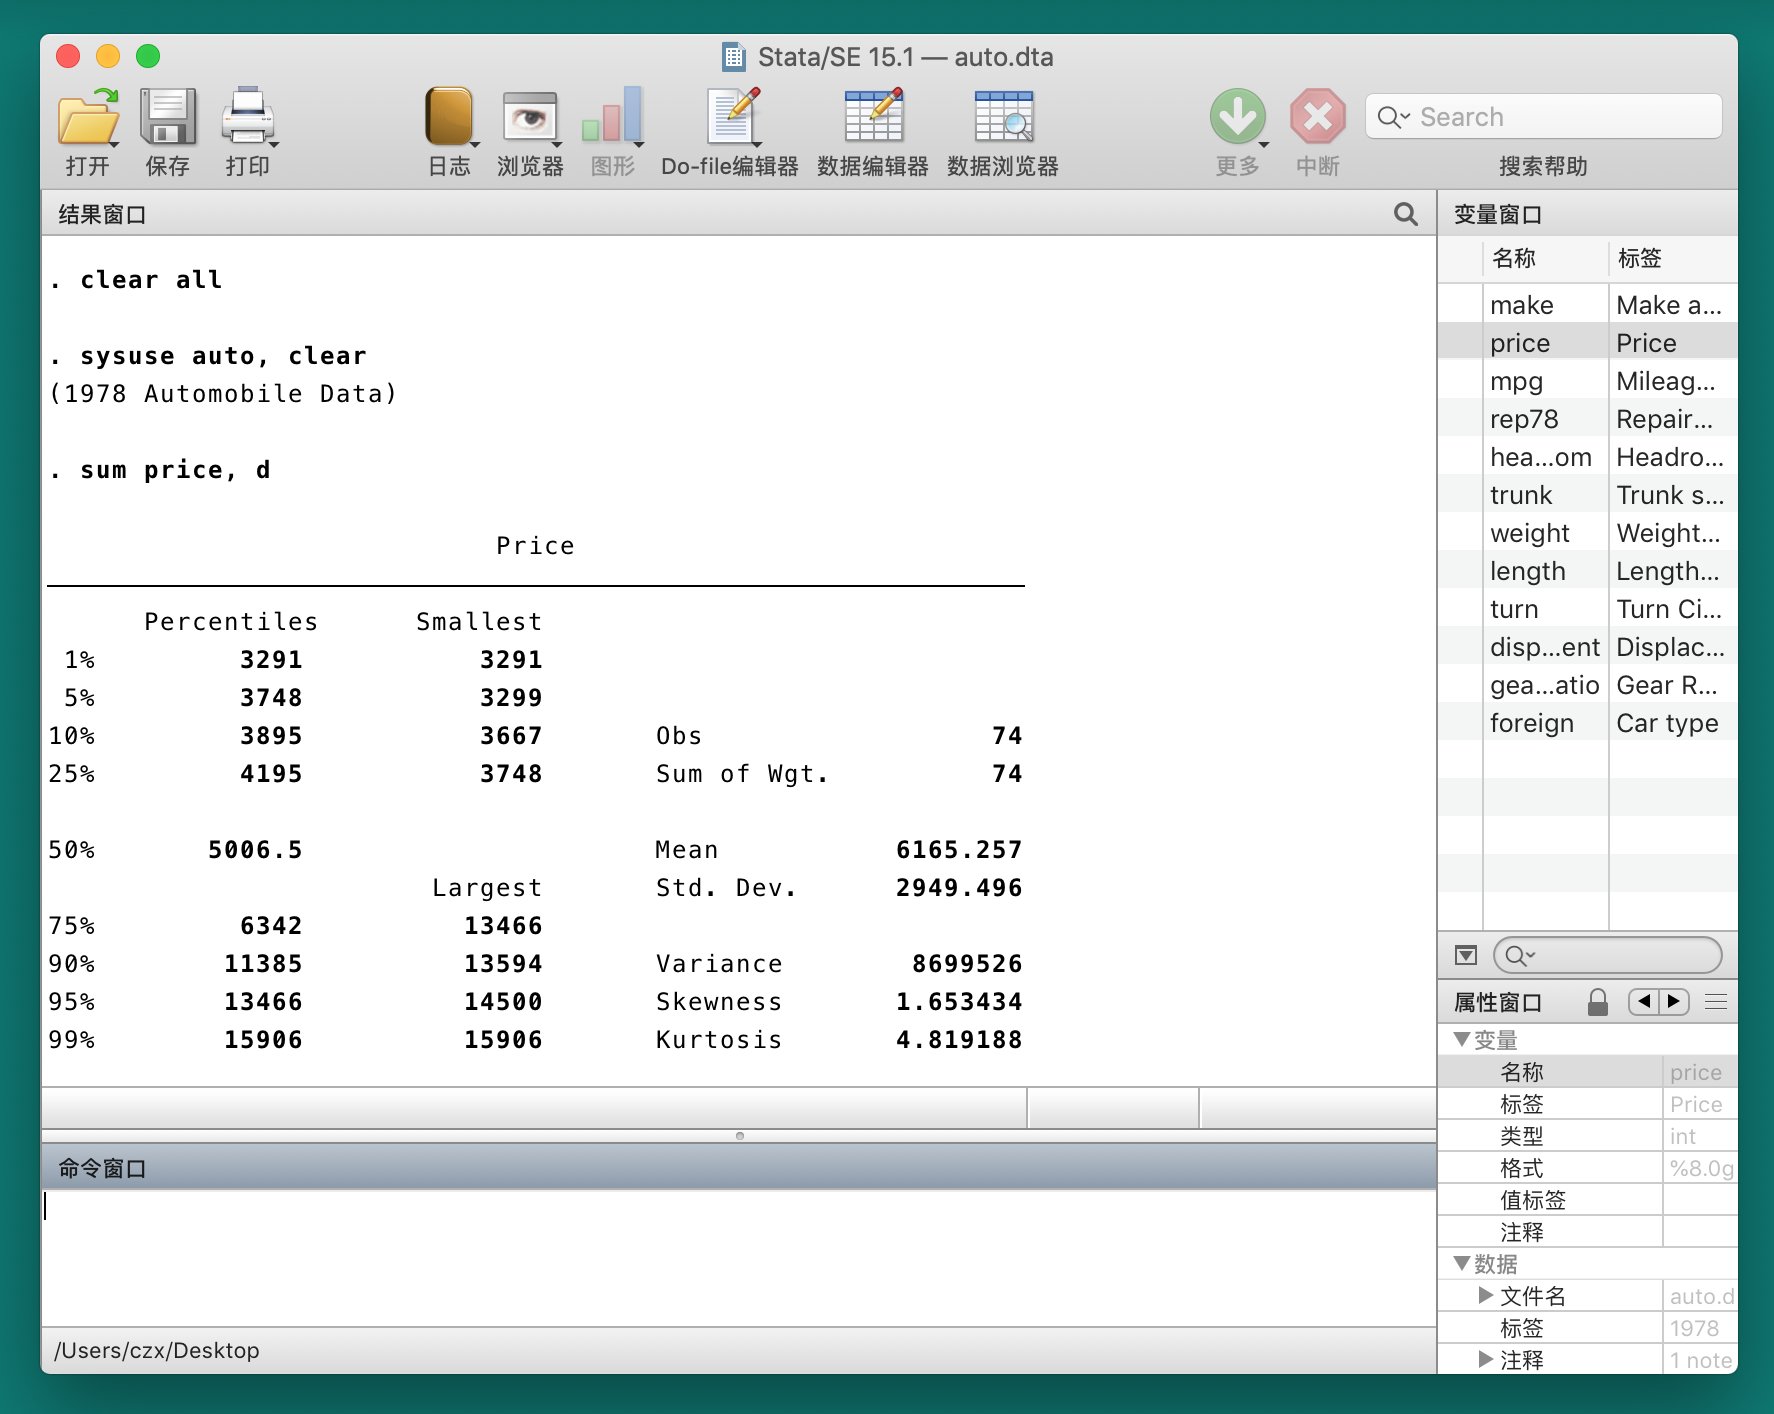
\includegraphics[width = \textwidth]{assets/stataui.png}
  \caption{Stata 15.1 for Mac 的界面}
  \label{fig:stataui}
\end{figure}

目前为止,你需要知道Stata最直接的使用方法是从命令窗口输入代码,然后回车运行,结果会显示在结果窗口。

如果你需要写很多行代码,这种使用方式就不是一个好习惯了,为了研究的可重复性,你最好建立一个 do 文件,然后将你的代码一行行输入在 do 文档里保存:

\begin{figure}[htbp]
  \centering
  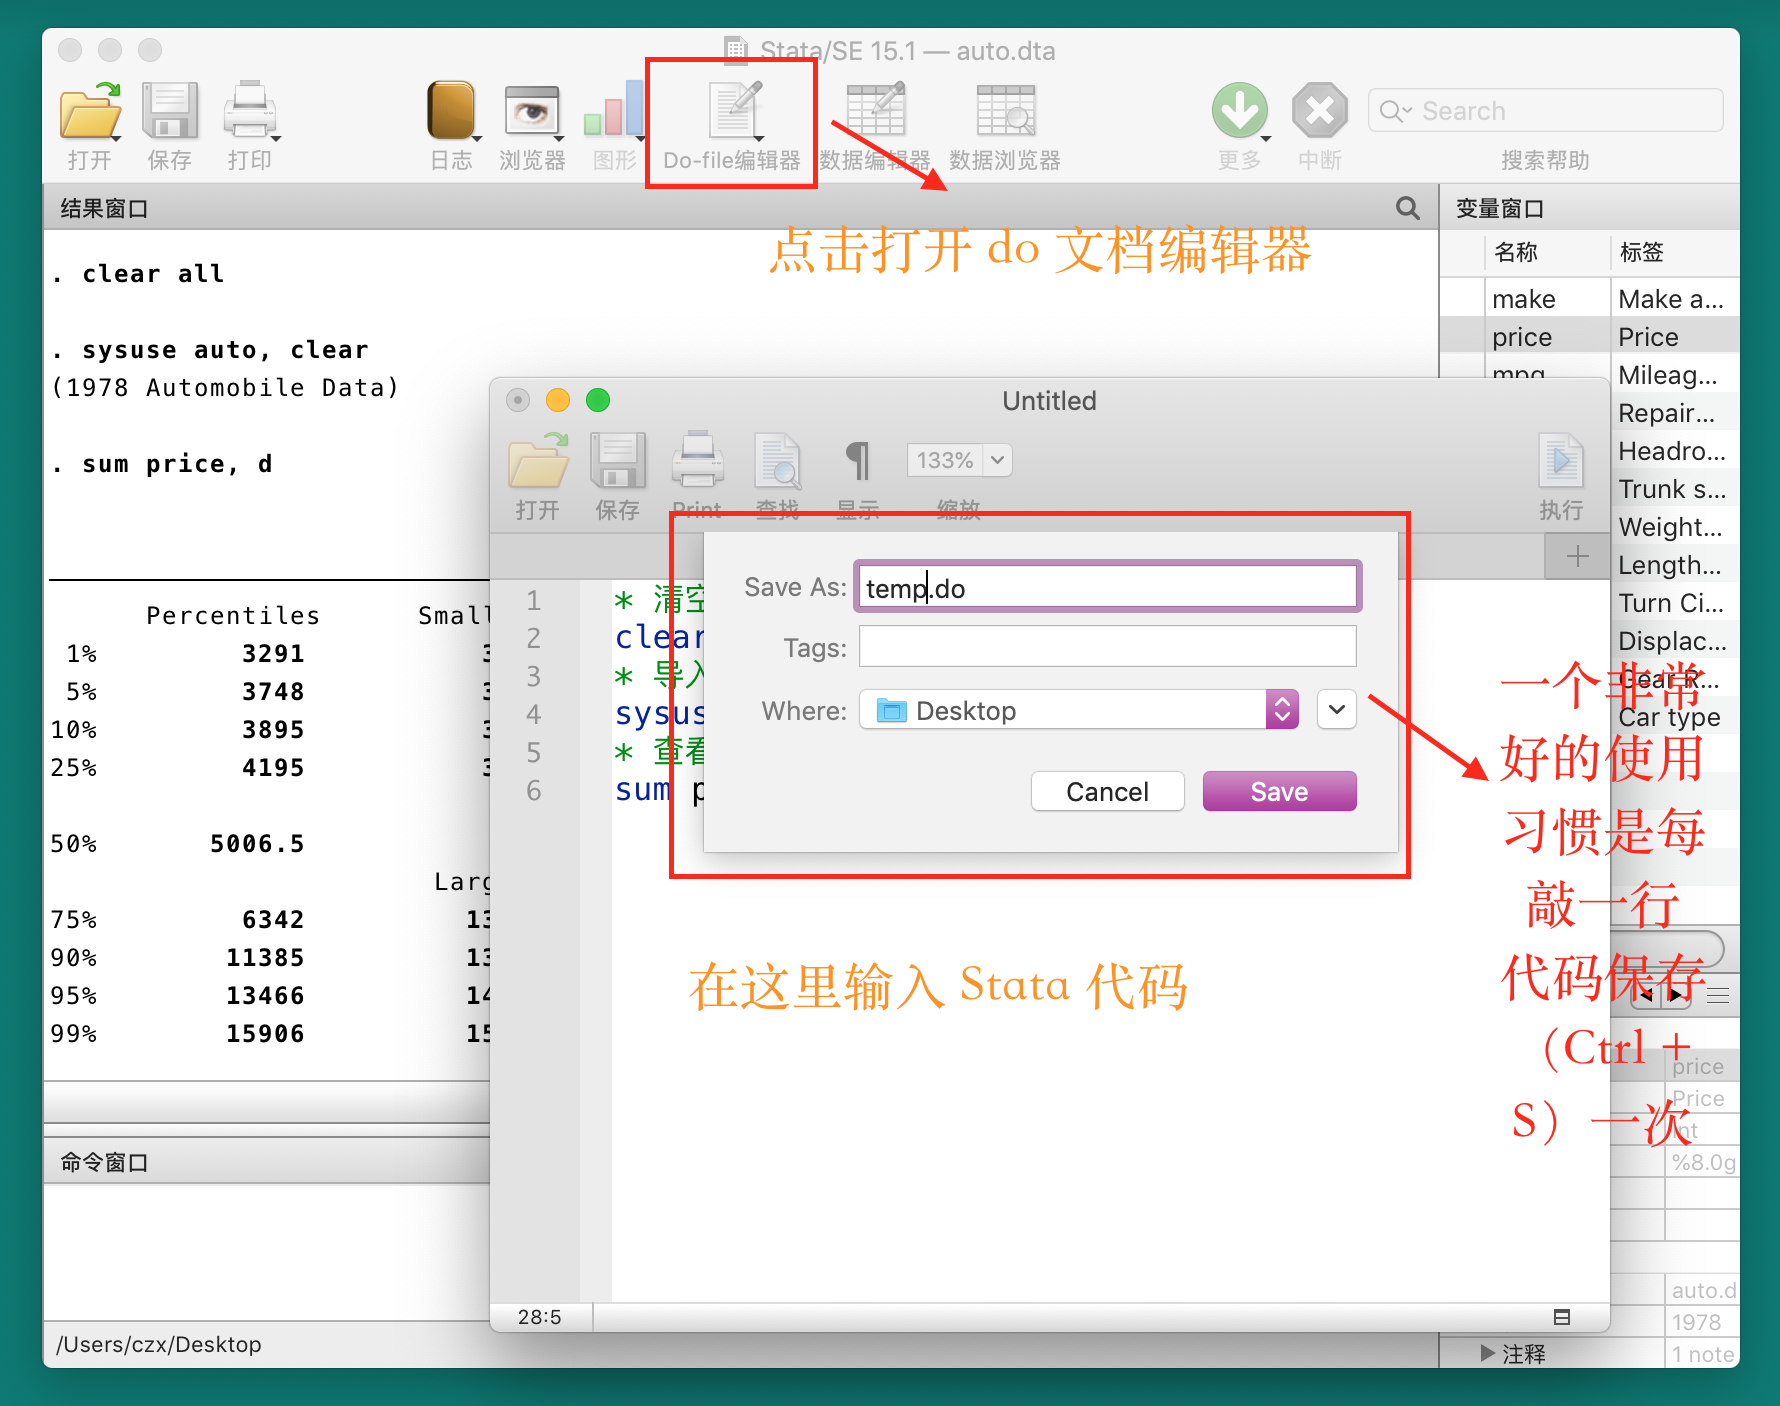
\includegraphics[width = \textwidth]{assets/do-file.png}
  \caption{Stata15.1 for Mac 的 do 文档编辑器界面}
  \label{fig:dofile}
\end{figure}

事实上,Stata 自带的这个编辑器并不好用,为了提高敲代码的效率,建议使用 Sublime Text3 编辑器。具体配置方法可以参考我的网站文章 \href{https://www.czxa.top/posts/59313/}{Stata安装与Sublime Text3配置教程}。

\begin{figure}[htbp]
  \centering
  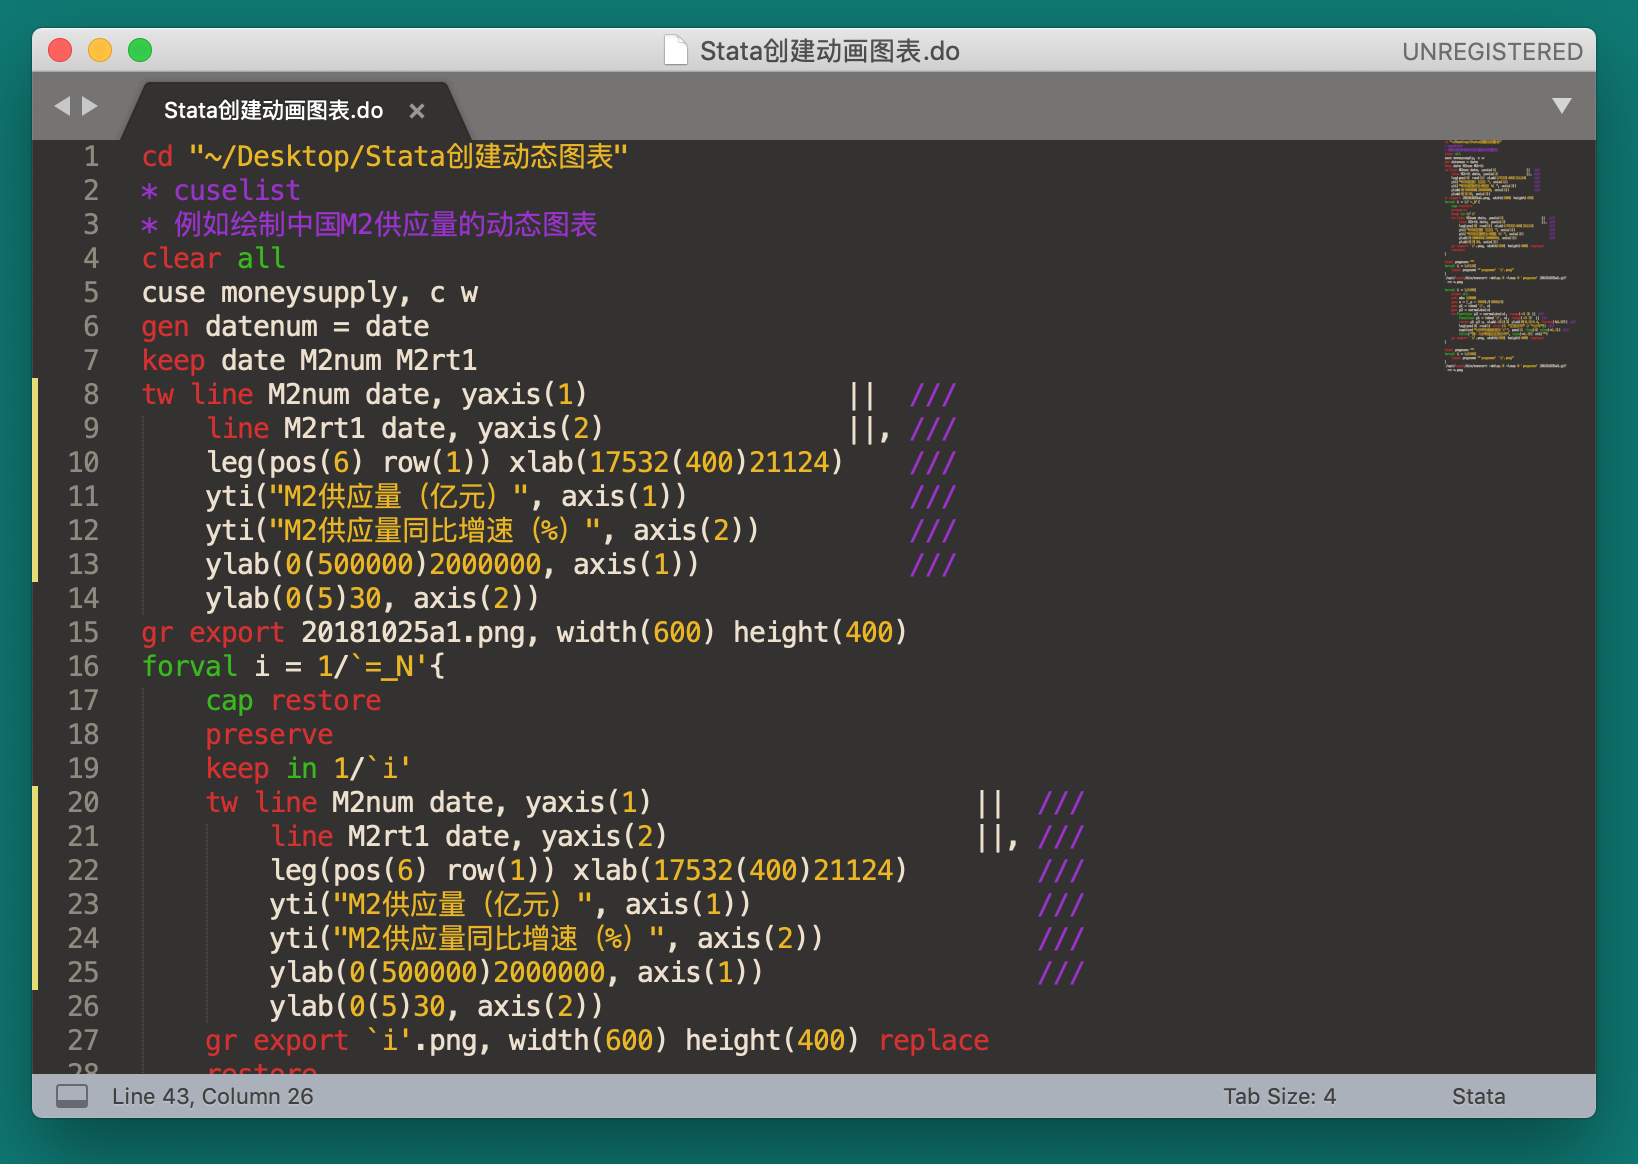
\includegraphics[width = \textwidth]{assets/sublime.png}
  \caption{Sublime Text3 for Mac 界面}
  \label{fig:sublime}
\end{figure}

你还可以从 \href{https://github.com/andrewheiss/SublimeStataEnhanced}{SublimeStataEnhanced} 获取最新的配置方法。

\section{stata4ds 命令包}

为了更方便的讲述,我开发了一个命令包,这个命令包涵盖了本书所需要的所有数据集和部分外部命令。你可以运行下面的 Stata 命令进行安装。

\begin{lstlisting}
  * 首先需要安装 github 命令,这个命令可以用来安装 GitHub 上的 Stata 命令。
  net install github, from("https://haghish.github.io/github/")
  * 然后使用 github 命令安装 stata4ds
  github install stata4ds, replace
\end{lstlisting}

除此之外,你还需要安装以下外部命令:

\begin{lstlisting}
  * 安装 cuse 命令包
  github install czxa/cuse, replace
  * 安装 finance 命令包
  github install czxa/finance, replace
  * 安装 tidy 命令包
  ssc install tidy, replace
  * 安装 superscatter 命令
  net install superscatter, from(http://digital.cgdev.org/doc/stata/MO/Misc) replace
  ...未完待续...
\end{lstlisting}

\begin{remark}
  实际上在安装 stata4ds 命令包的最后这些命令会被自动逐一地安装。
\end{remark}

\section{运行 Stata 代码}

前面一节展示了一段 Stata 代码的运行结果,在本书中的代码是像这样的:

\begin{lstlisting}
  display 1 + 2
  *> 3
\end{lstlisting}

而你运行上面的代码之后,结果窗口显示的结果应该是这样的:

\begin{lstlisting}
  . display 1 + 2
  3
\end{lstlisting}

\section{获取帮助}

Stata 提供了非常详细完善的帮助文档,要查阅帮助文档,你可以使用 \textcolor{third3}{help} 命令,例如查看 \textcolor{third3}{clear} 的帮助文档:

\begin{lstlisting}
help clear
\end{lstlisting}

\begin{figure}[htbp]
  \centering
  
\includegraphics[width = 0.6\textwidth]{assets/clear.png}
  \caption{clear 命令的帮助文档}
  \label{fig:clear}
\end{figure}

Stata 还拥有着丰富的网络资源,你可以使用 \textcolor{third3}{search} 和 \textcolor{third3}{findit} 命令搜索,例如我想查找 \textcolor{third3}{egen} 相关的内容:

\begin{lstlisting}
  search egen
  findit egen
\end{lstlisting}

Stata 官网上也有着丰富的 Stata 资源。此外,Stata15 比起前代的 Stata 有巨大的进步,如果你想了解 Stata15 的新功能,可以到 Stata 的官网查看:\href{https://www.stata.com/new-in-stata/}{New in Stata 15}。

\begin{figure}[htbp]
  \centering 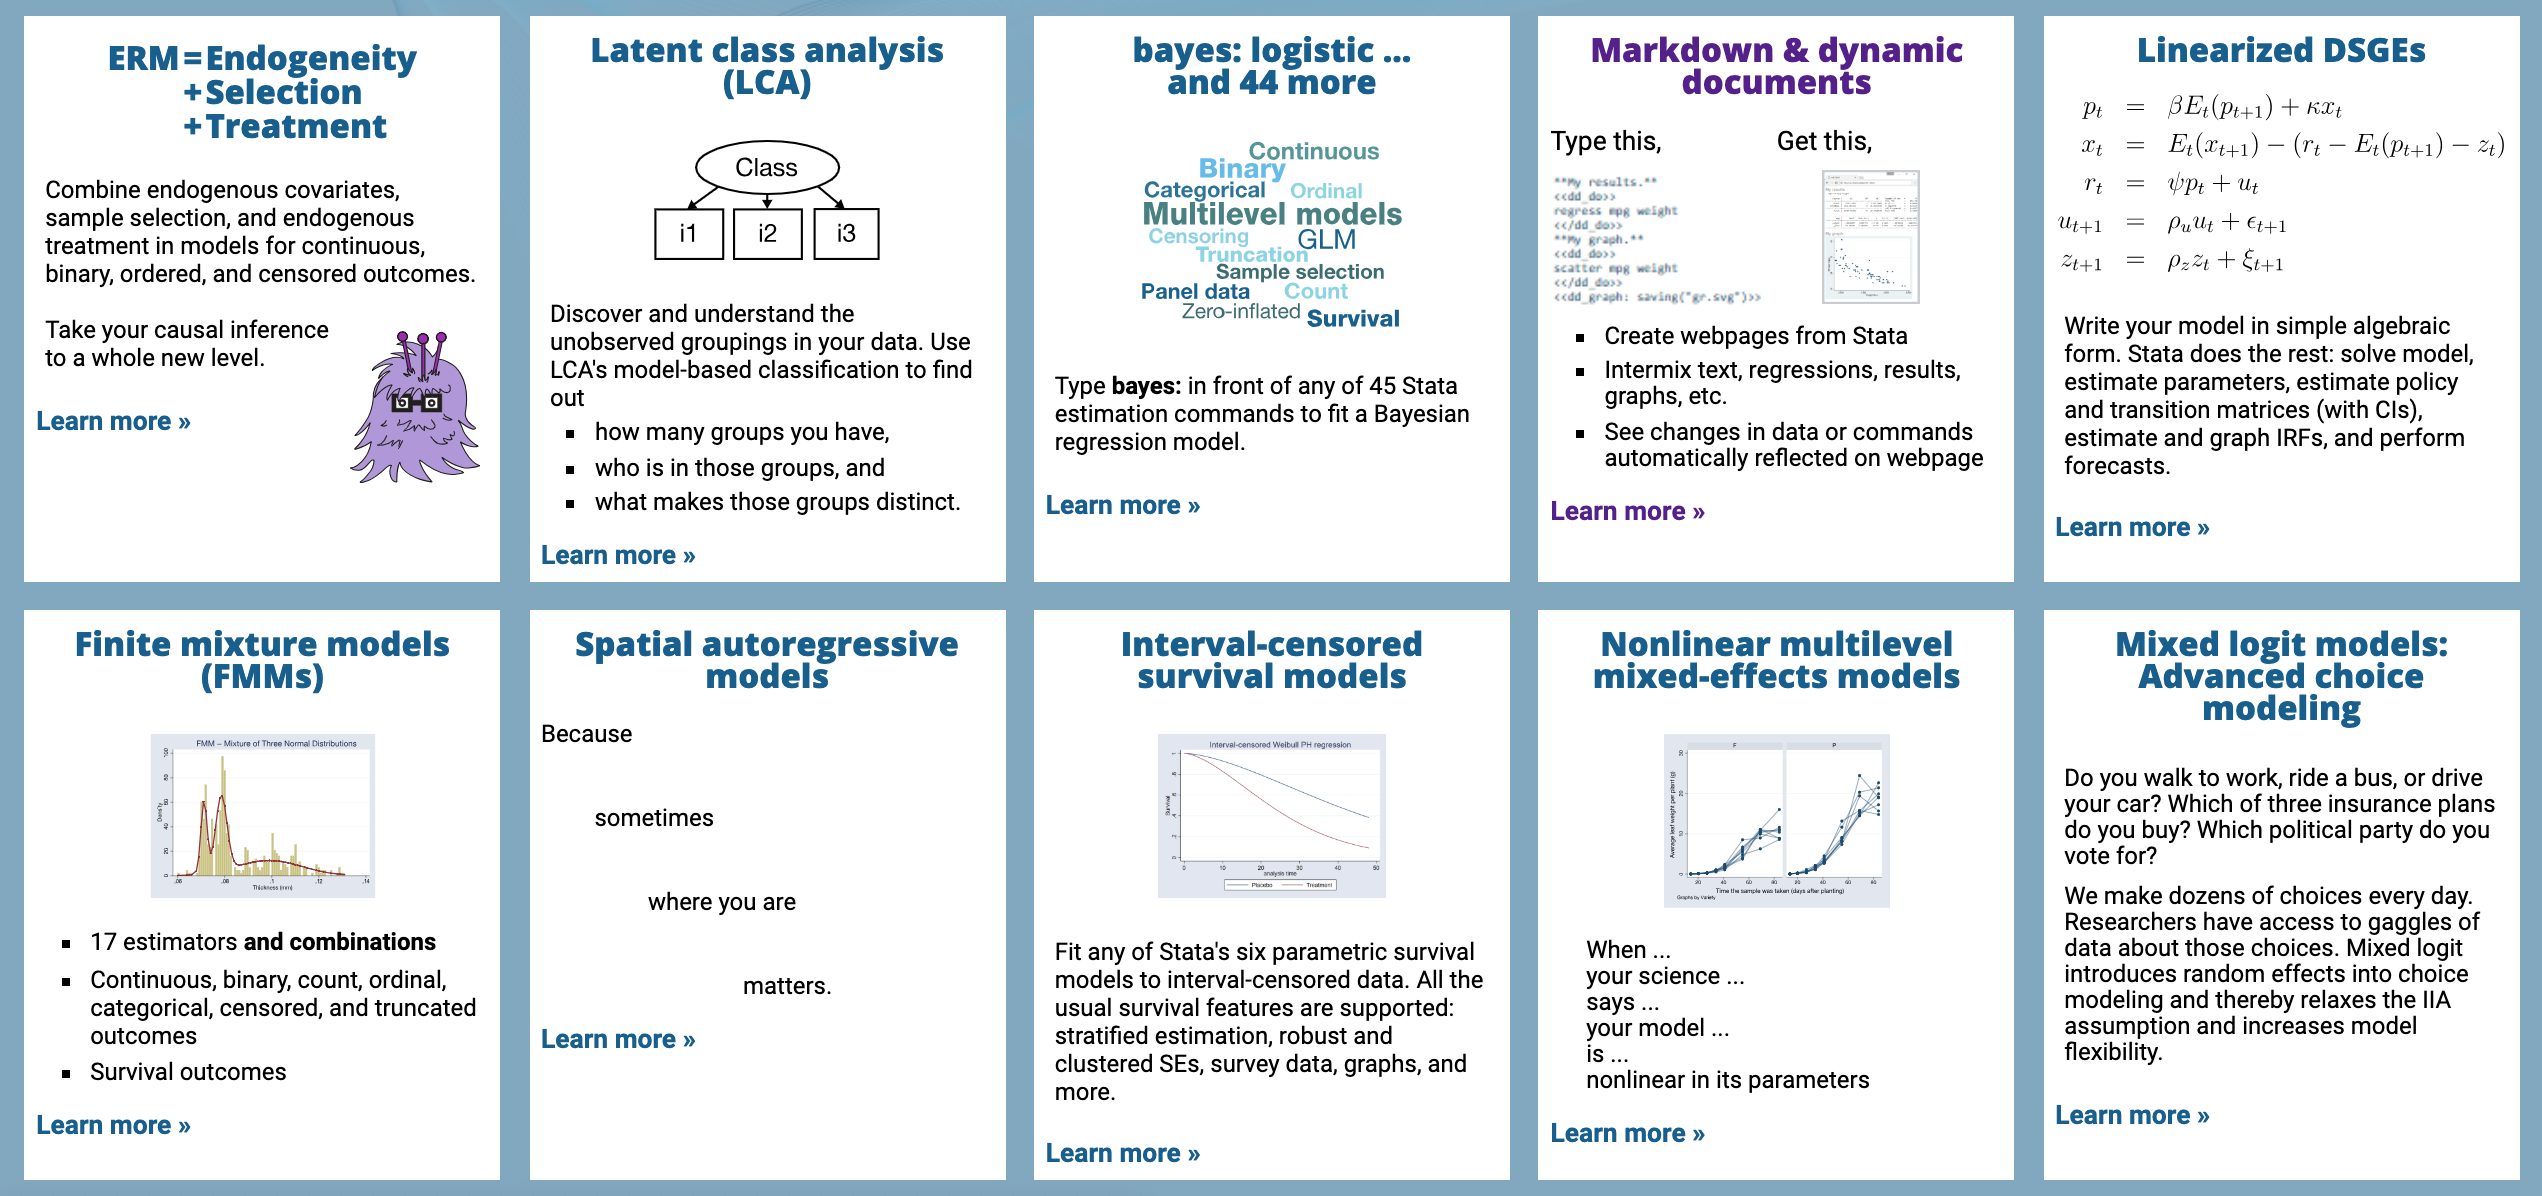
\includegraphics[width= 0.8\textwidth]{assets/newinstata15.png}
  \caption{Stata15 的新功能}
  \label{fig:newinstata15}
\end{figure}

你还可以在 \href{https://www.statalist.org/forums/}{Stata List} 和 \href{https://blog.stata.com/}{Stata Blog} 获取 Stata 使用的资源和帮助。另外, \href{https://github.com/topics/stata}{GitHub \# Topic: stata} 上也有一些非常好用的 Stata 命令和学习资源。

下一章实际上并不是本书想要编排进来的内容,而是作者之前在担任计量经济学助教的时候编写的讲义,虽然比较粗略(毕竟讲义这种东西的目的只是帮助演讲者组织思路)。但是我相信通过下一章内容的学习,你将能够更轻松的进行本书的学习。因此特意将该讲义插入进来(其实只是想凑字数)。

\chapter{Stata 基础操作}
\section{Stata 是什么?}

根据 Stata 对自己的介绍:

\begin{quote}
\begin{enumerate}
\item  Stata is a statistical package for managing, analyzing, and graphing data.
\item  Stata is available for a variety of platforms. Stata may be used either as a point-and-click application or as a command-driven package.
\item  Stata's GUI provides an easy interface for those new to Stata and for experienced Stata users who  wish to execute a command that they seldom use.
\item  The command language provides a fast way to communicate with Stata and to communicate more complex ideas.
\end{enumerate}
\end{quote}

也就是说, Stata 是一个集数据管理、分析和可视化的工具。可以在各种操作系统中使用,可以通过鼠标点击操作也能通过命令行驱动。

Stata 的图形用户界面让新手们很方便入门,Stata 的命令语言使得很多复杂的想法变得容易实现。

我经常看到很多 R、Python、Matlab 用户对 Stata 非常不屑一顾。每每提及 Stata 总是要加一句:

\begin{quote}
``如果Stata也算编程语言的话······''
\end{quote}

我也常听一些没有接触过编程的朋友对Stata望而却步,他们常说:

\begin{quote}
``虽然看不懂,但是觉得很厉害的样子。''
\end{quote}

所以Stata是什么?在 Stata 中运行 \texttt{help\ class} 命令你就可以看到下面的一段介绍:

\begin{quote}
Stata's two programming languages, ado and Mata, each support object-oriented programming. {[}P{]} class explains object-oriented programming in ado. Most users interested in object-oriented programming will wish to do the programming in Mata. See {[}M-2{]} class to learn about object-oriented programming in Mata.
\end{quote}

Stata 是套体系完整的面向对象的编程语言。两种编程语言,\textbf{ado} 和 \textbf{Mata} ,第一种较为常用,第二种更为强大。

\section{Stata 能做什么?}

\begin{enumerate}
\item  数据获取与处理。使用Stata可以比较快速的获取多种数据并迅速整理成研究者所需要的数据。
\item  精美统计图形绘制与导出。Stata的绘图系统是相当完整的。通过绘图主题的选择,Stata作图也可以非常的精美。
\item  严谨可重复的实证研究。
\end{enumerate}

在熟练使用 Stata 之前,你的论文原材料可能是像图 \ref{fig:dirtydir}一样的(图 \ref{fig:dirtydir} 并不是论文的原材料,是我随便截的,只是想表达乱):

\begin{figure}[htbp]
  \centering 
\includegraphics[width=0.9\textwidth]{assets/dirtydir.png}
  \caption{一个乱七八糟的文件夹}
  \label{fig:dirtydir}
\end{figure}

在此之前可能你的主要数据处理工具是 Excel ,并且还不会 Excel VBA ,所以经常会整夜整夜的复制粘贴。而这些工作实际上用几行 Stata 语句就能完成。

那你用熟练了 Stata 之后你的论文数据是什么样的呢?假如你是一个像我一样的强迫症患者,那么你的论文源码将会像图 \ref{fig:cleandir} 一样。

\begin{figure}[htbp]
  \centering 
\includegraphics[width=0.9\textwidth]{assets/cleandir.png}
  \caption{一个整洁的项目文件夹}
  \label{fig:cleandir}
\end{figure}

这个文件夹的目录结构是:

\begin{lstlisting}
  .
  ├── ADO
  │   ├── carryforward.ado
  │   ├── carryforward.hlp
  │   ├── estadd.ado
  │   ├── estadd.hlp
  │   ├── esttab.ado
  │   └── esttab.hlp
  ├── DATA
  │   ├── beta.csv
  │   └── mydata.dta
  ├── DO
  │   ├── 表2-1-描述性统计表.do
  │   ├── 表3-1-模型估计结果.do
  │   ├── 图3-1-每个月份的风险暴露变化对股票流动性影响的差异.do
  │   ├── 表3-2-模型估计结果.do
  │   ├── 图3-2-每个年份风险暴露变化对股票流动性影响的差异.do
  │   ├── 表4-1-稳健性检验结果.do
  │   └── 设定绘图主题.do
  ├── DOCS
  │   └──  风险暴露的变化对股票流动性的影响.pdf
  ├── IMAGE
  │   ├── 年份效应.png
  │   └── 月份效应.png
  ├── 主程序.do
  └── 参考文献
      └── 110228635.pdf
\end{lstlisting}

在用Stata之前,每次画图你可能都要在 Excel 上面点击无数次。而用 Stata 之后,即使是下面这样复杂的图\ref{fig:sci},你只需要一行命令就能绘制出来:

\begin{figure}[htbp]
  \centering 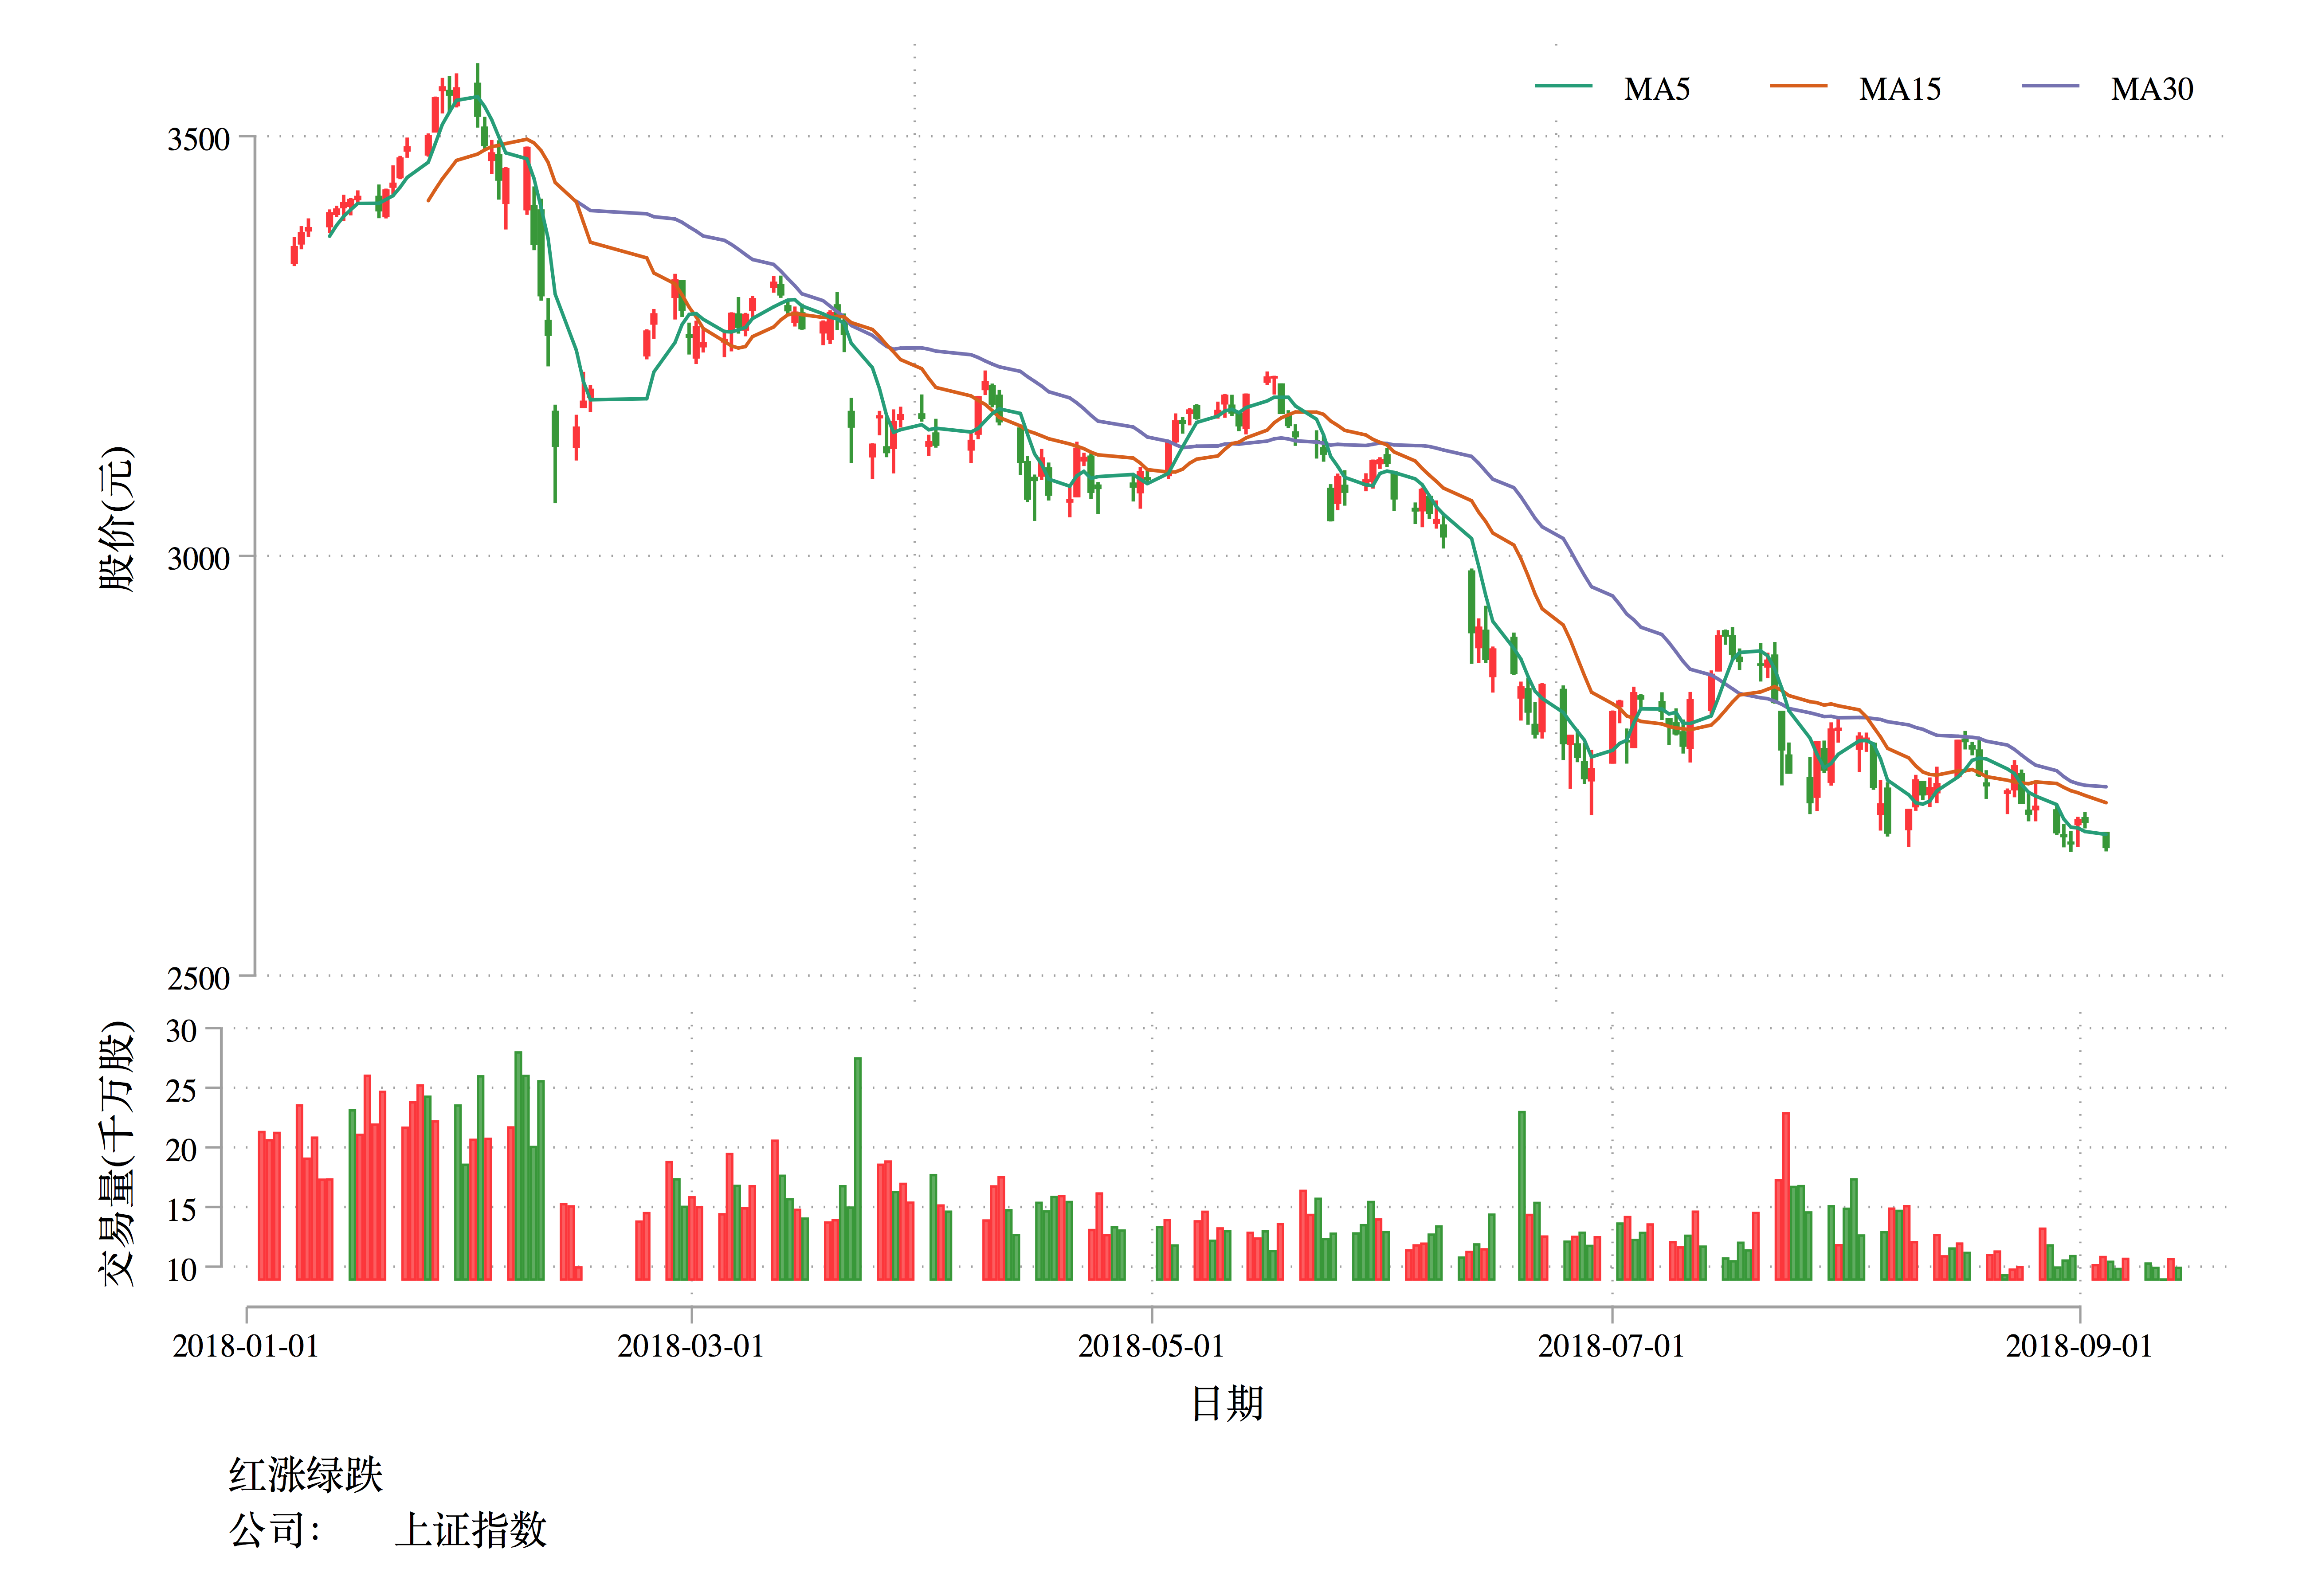
\includegraphics[width=0.9\textwidth]{assets/stkpv4.png}
  \caption{上证指数蜡烛图}
  \label{fig:sci}
\end{figure}

此外,如果你还会一些数据库或其它编程软件,Stata能够很好的和它们交互使用。

如果说 Stata 不是最好的,我觉得 Stata 是做实证研究的最好工具。

\begin{enumerate}
\item  Stata 作为商业软件,有着专业且负责的团队维护。所以 Stata 的帮助文档是最让人喜爱的,这些也是很多开源软件无法比拟的。
\item  Stata 的速度相对较快,Stata的启动速度远快于 Matlab、SAS 这些软件,且对电脑硬件要求较低,这是非常重要的,如果你想用一个软件,然后打开它就要等待几分钟。那我想你可能很快就烦了。另外 Stata 运行的速度也足够快。可以满足大多数用户的需要。
\item  Stata 提供了很多可以把统计表格导出到 Word、PDF 和 Tex 文档的命令。实际上 Stata15 的 putdocx 命令搭配其它的一些命令可以直接实现论文的编排。
\end{enumerate}

我想以上的每一条都足以成为大家认真学习 Stata 的理由。

下面就让我们进入Stata的世界吧!

\section{Stata 基本操作}
\subsection{Stata 系统文件夹}

运行 \lstinline{sysdir} 命令即可得到 Stata 的系统文件夹列表:

\begin{lstlisting}
sysdir
*>    STATA:  /Applications/Stata15/
*>     BASE:  /Applications/Stata15/ado/base/
*>     SITE:  /Applications/Stata15/ado/site/
*>     PLUS:  /Users/czx/Library/Application Support/Stata/ado/plus/
*> PERSONAL:  /Users/czx/Library/Application Support/Stata/ado/personal/
*> OLDPLACE:  ~/ado/
\end{lstlisting}

\begin{itemize}
\item  \texttt{BASE} 文件夹包含了Stata官方的 ado 文件;
\item  \texttt{PERSONAL} 文件夹可以放置你自己的 ado-files;
\item  \texttt{PLUS} 文件夹在你下载外部命令时会被自动创建。
\end{itemize}

另外运行 \texttt{adopath} 也可以得到:

\begin{lstlisting}
adopath
*>  [1]  (BASE)      "/Applications/Stata15/ado/base/"
*>  [2]  (SITE)      "/Applications/Stata15/ado/site/"
*>  [3]              "."
*>  [4]  (PERSONAL)  "/Users/czx/Library/Application Support/Stata/ado/personal/"
*>  [5]  (PLUS)      "/Users/czx/Library/Application Support/Stata/ado/plus/"
*>  [6]  (OLDPLACE)  "~/ado/"
\end{lstlisting}

\texttt{adopath} 命令的运行结果和 \texttt{sysdir} 基本相同,这里的排序也是 \texttt{Stata} 寻找 \texttt{ado} 文件的顺序。

\subsection{数据导入}
\subsubsection{导入系统数据集}

系统数据集就是位于系统文件夹的数据集,这些数据集一般是一些示例数据集。导入系统数据集是使用sysuse命令,最有名的系统数据集要数auto数据集了:

\begin{lstlisting}
sysuse auto, clear
\end{lstlisting}

这是个1978年的汽车数据集。这个数据集是这样的:

\begin{figure}[htbp]
  \centering 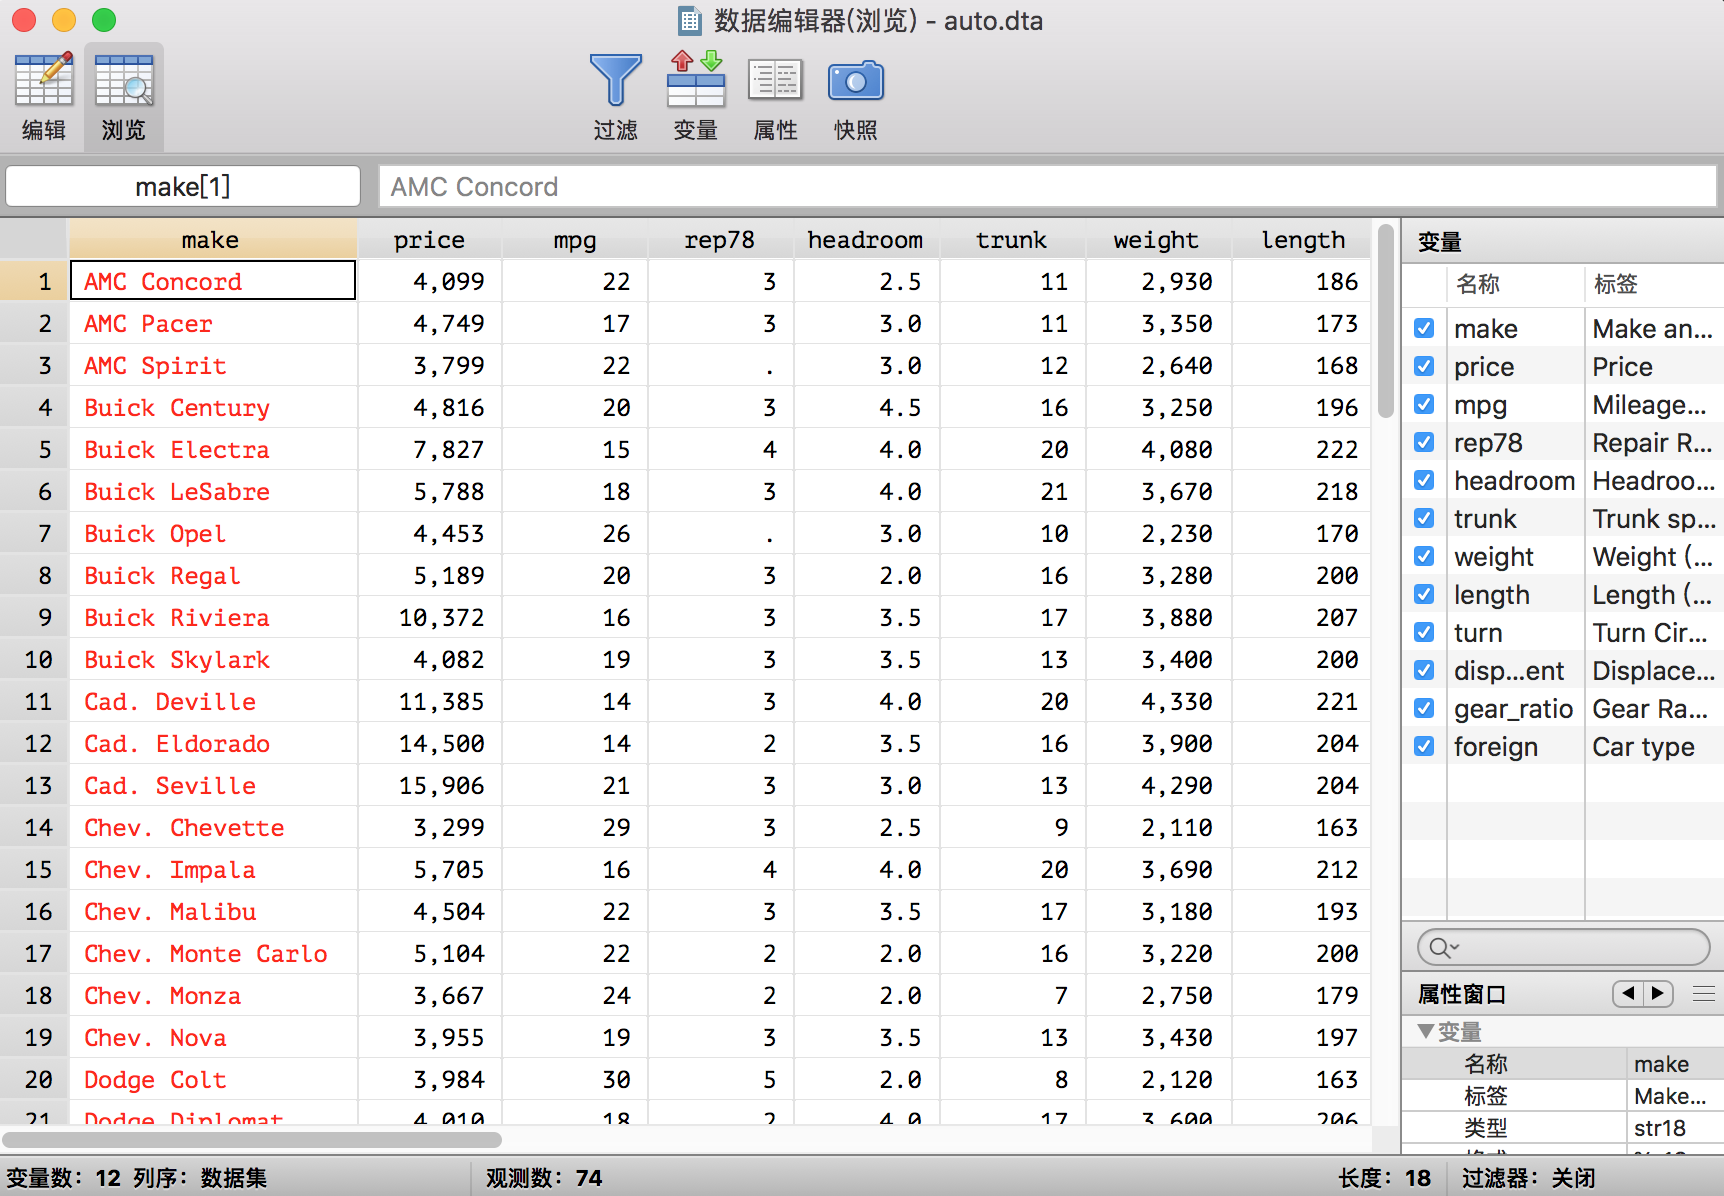
\includegraphics[width=0.9\textwidth]{assets/auto}
  \caption{1978年汽车数据集}
  \label{fig:auto}
\end{figure}

此外sysuse还可以用来查看所有的系统数据集:

\begin{lstlisting}
sysuse dir
*>  .dta               cjd1617.dta        lifeexp.dta        reshape1.dta
*>  air2.dta           colorschemes.dta   lutkepohl2.dta     sandstone.dta
*>  airq.dta           countycode.dta     moneysupply.dta    sexratio.dta
*>  auto.dta           educ99gdp.dta      network1.dta       smoking.dta
*>  auto2.dta          fullauto.dta       network1a.dta      sp500.dta
*>  autornd.dta        ghanaage.dta       nhanes2f.dta       splotxmpl.dta
*>  bplong.dta         gnp96.dta          nlsw88.dta         stackxmpl.dta
*>  bpwide.dta         grunfeld.dta       nlswide1.dta       surface.dta
*>  brewmeta.dta       houseprice.dta     nlswork.dta        tsline1.dta
*>  cancer.dta         jd14151617xxb.dta  nlswork2.dta       tsline2.dta
*>  census.dta         jd141516cjd.dta    parent.dta         uslifeexp.dta
*>  child.dta          jd2017zsjh.dta     pop2000.dta        uslifeexp2.dta
*>  citytemp.dta       jdcourse2018a.dta  population.dta     voter.dta
*>  citytemp4.dta      lbw.dta            rate2.dta          xtline1.dta
\end{lstlisting}

使用all选项可以查看所有的:

\begin{lstlisting}
sysuse dir, all
*>  .dta                  child.dta             network1a.dta
*>  __i10v2003.dta        china_map.dta         nhanes2f.dta
*>  __i10v2004.dta        citytemp.dta          nlsw88.dta
*>  __i10v2006.dta        citytemp4.dta         nlswide1.dta
*>  __i10v2007.dta        cjd1617.dta           nlswork.dta
*>  __i10v2008.dta        colorschemes.dta      nlswork2.dta
*>  __i10v2009.dta        countycode.dta        parent.dta
*>  __i10v2010.dta        echarts_worldmap.dta  pop2000.dta
*>  __i10v2011.dta        educ99gdp.dta         population.dta
*>  __i10v2012.dta        fullauto.dta          rate2.dta
*>  __i10v2013.dta        ghanaage.dta          reshape1.dta
*>  __i10v2014.dta        gini_prov.dta         sandstone.dta
*>  __i10v2016.dta        gnp96.dta             sexratio.dta
*>  __icd10.dta           grunfeld.dta          smoking.dta
*>  __icd10cm.dta         houseprice.dta        sp500.dta
*>  __icd10pcs.dta        icd9_cod.dta          splotxmpl.dta
*>  air2.dta              icd9_cop.dta          stackxmpl.dta
*>  airq.dta              jd14151617xxb.dta     surface.dta
*>  auto.dta              jd141516cjd.dta       tsline1.dta
*>  auto2.dta             jd2017zsjh.dta        tsline2.dta
*>  autornd.dta           jdcourse2018a.dta     uslifeexp.dta
*>  bplong.dta            lbw.dta               uslifeexp2.dta
*>  bpwide.dta            lifeexp.dta           voter.dta
*>  brewmeta.dta          lutkepohl2.dta        xtline1.dta
*>  cancer.dta            moneysupply.dta
*>  census.dta            network1.dta
\end{lstlisting}

\subsubsection{导入网络数据集}

网络数据集是存放在 Stata 公司服务器上的一些数据集,通常也是一些示例数据集。例如导入 \texttt{lifeexp.dta} 数据集:

\begin{lstlisting}
webuse lifeexp, clear
*> (Life expectancy, 1998)
\end{lstlisting}

这是一个1998年预期寿命数据集,括号里面的内容是数据集的标签(\lstinline{help label})。

\lstinline{webuse query}可以用来查看当前webuse指向的数据仓库地址:

\begin{lstlisting}
webuse query
*> (prefix now "http://www.stata-press.com/data/r15")
\end{lstlisting}

还可以换个地址:

\begin{lstlisting}
webuse set "https://czxa.github.io/cuse/c"
*> (prefix now "https://czxa.github.io/cuse/c")
\end{lstlisting}

这个网址是我的数据仓库下的一个名称为 c 的子文件夹,里面放置着 c 开头的数据集。设定好网址指向之后就可以调用该指向下的数据集了:

\begin{lstlisting}
webuse cjd1617, clear
*> (金融学16和17年成绩单)
\end{lstlisting}

这是我们班同学2016和2017年的成绩单,为了保护隐私,我抹去了大家的姓名。
重新把webuse的指向的网址指向设定为默认网址,只需要运行下面的命令即可:

\begin{lstlisting}
webuse set
*> (prefix now "http://www.stata-press.com/data/r15")
\end{lstlisting}

\subsubsection{调用我的个人仓库里面的数据集}
在实际数据处理过程中,有时候我们会需要一些常用的数据集,例如中国行政区划编码。如果每次我们都上网找然后再导入 Stata 进行整理,是不是太麻烦了?我们能不能像 sysuse、webuse 这样直接使用数据呢?所以我就写了这套 \lstinline{cuse} 命令。这个命令里面包含了很多我经常使用的数据集,例如各省市的行政区号之类的。

运行下面的命令即可安装这个命令:

\begin{lstlisting}
github install czxa/cuse, replace
\end{lstlisting}

这个命令的使用方法是:

\begin{lstlisting}
* cuselist可以用来查看数据库中包含的数据
cuselist
*> 【0】
*> ----------------------------------------------------------------------
*> 1.  000001.dta: 平安银行历史股票数据
*> 【a】
*> ----------------------------------------------------------------------
*> 1.  amricancellmapdata.dta: 美国蜂窝地图各个省份的位置坐标
*> 【c】
*> ----------------------------------------------------------------------
*> 1.  cellmapdata.dta: 中国蜂窝地图各个省份的位置坐标
*> 1.  countycode.dta: 中国各省市区县编号(即身份证前六位号码)
*> 2.  china_label.dta: 中国地图标签
*> 3.  china_map.dta: 中国地图数据
*> 4.  china_city_spatial_distance.dta: 中国地级地图数据集
*> 5.  china_province_spatial_distance.dta: 中国省级地图数据集
*> 6.  cjd1617.dta: 金融学16和17年成绩单
*> 7.  cpi.dta: 中国CPI2008/1-2017/11
*> 8.  countrysexratio.dta: knoema各国总人口性别比例数据
*> 9.  ctbc2.dta: 中债国债2002-2017年国债到期收益率
*> 10.  cnstockholiday.dta: 上交所与深交所休市日期
*> 11.  cnstockincome.dta:1989年-2017年所有上市公司的基本收入状况
*> ----------------------------------------------------------------------
*> 【d】
*> ----------------------------------------------------------------------
*> 1.  echarts_worldmap.dta: ECharts世界地图各国中英文名称对照
*> 【g】
*> ----------------------------------------------------------------------
*> 1.  gdpjdlj.dta: 中国GDP季度累计2006/第一季度-2017/第三季度
*> 2.  gini_prov.dta: 1995-2010中国各省份Gini系数
*> 【h】
*> ----------------------------------------------------------------------
*> 1.  huaihe.dta: 2017年淮河供暖政策对人预期寿命的影响模仿数据集
*> 2.  houseprice.dta: 中国百城房价数据集
*> ----------------------------------------------------------------------
*> 【j】
*> ----------------------------------------------------------------------
*> 1.  jdcourse2018a.dta: 2018年上半年暨南大学排课选课表
*> 2.  jd2017zsjh.dta: 暨南大学2017年各省招生人数
*> ----------------------------------------------------------------------
*> 【l】
*> ----------------------------------------------------------------------
*> 1.  life_expentancy.dta: 2010年中国各省市自治区人口出生时预期寿命
*> 【m】
*> ----------------------------------------------------------------------
*> 1.  moneysupply.dta: 2008/1-2017/11中国货币供应量M0M1M2
*> ----------------------------------------------------------------------
*> 【p】
*> ----------------------------------------------------------------------
*> 1.  pm10.dta: 2017年淮河供暖政策对人预期寿命影响的原始数据集
*> 2.  population.dta: 2010年中国各区县人口
*> 3.  population_prov.dta: 2002-2014年全国各省市年末人口
*> 4.  pjw.dta: 分城市人口、就业与工资(1990-2016)
*> ----------------------------------------------------------------------
*> 【s】
*> ----------------------------------------------------------------------
*> 1.  station.dta: 中国所有火车站车站代码
*> 2.  smoking.dta: 合成控制法的美国39个洲的香烟销售量数据集
*> 2.  sexratio.dta: knoema各国总人口性别比例数据
*> ----------------------------------------------------------------------
*> 【t】
*> ----------------------------------------------------------------------
*> 1.  titanic.dta: 泰坦尼克号生存数据集
*> 2.  tourism.dta: 旅游事业发展情况
*> ----------------------------------------------------------------------
*> 【书籍数据集】
*> 注意!如果你想调用的数据集的名字里含大写字母,你需要把它的首字母调成小写才能调用!
*> 1. 《计量经济学及Stata应用》——陈强著
*> 2. 《高级计量经济学及Stata应用》——陈强著
*> 3. 《An Introduction to Stata Programming, Second Edition》——Christopher F. Baum著
\end{lstlisting}

然后如果你想调用需要的数据集,使用 cuse 命令,这个命令的语法是:

\begin{quote}
cuse filename , {[}clear web savetosystem{]}
\end{quote}

下划线表明该选项可以简写为下划线部分。

\begin{itemize}
\item  clear:清空当前数据集;
\item  web:表示从网络读取数据,对我的电脑来说,这是个可选项,对于别人的电脑来说,这是个必选项。
\item  savetosystem表示调用的同时把该数据集存入系统文件夹。
\end{itemize}

例如,假如我想调用 \texttt{grilic\_small.dta} 数据集,使用下面的命令即可:

\begin{lstlisting}
cuse grilic_small, c w s
\end{lstlisting}

上面的命令就实现了把内存清空、从网络获取数据和存入系统文件夹三个操作,以后如果需要这个数据集,用sysuse也可以读取了:

\begin{lstlisting}
sysuse grilic_small, clear
\end{lstlisting}

\subsection{读入dta数据集}
这个是最为常用的命令, use 命令。用来导入 Stata 的 dta 格式的数据集。

例如我想读取\texttt{grilic\_small.dta}数据集,下面的命令即可:

\begin{lstlisting}
* 首先把工作目录设置到这个数据集所在的文件夹
cd ~/Desktop/datasets
* 然后使用use命令读取该数据集
use grilic_small, clear
* 当然你也可以这么做,也就是路径+文件名
use ~/Desktop/datasets/grilic_small.dta, clear
* 但是不推荐。建议的工作流程是把所有的工作都在工作目录下进行。
\end{lstlisting}

\subsection{读入csv数据集}
csv格式的数据集是逗号分隔的文本文件,可以直接用Excel打开。例如,我想读取 \texttt{pingan.csv} 文件,这个文件下载地址为:\texttt{https://czxb.github.io/mr/pingan.csv} 。

Stata的copy命令可以被用来下载文件:

\begin{lstlisting}
copy "https://czxb.github.io/mr/pingan.csv" pingan.csv, replace
\end{lstlisting}

然后你就能在你的工作目录里面发现这个文件了。如果你不清楚你的工作目录在哪里,可以运行下面的命令:

\begin{lstlisting}
pwd
*> /Users/czx/Desktop
\end{lstlisting}

然后我们把这个csv文件读入Stata:

\begin{lstlisting}
import delimited using pingan.csv, clear
\end{lstlisting}

此外,你还可以通过 GUI (图形用户界面) 导入:

\begin{figure}[htbp]
  \centering 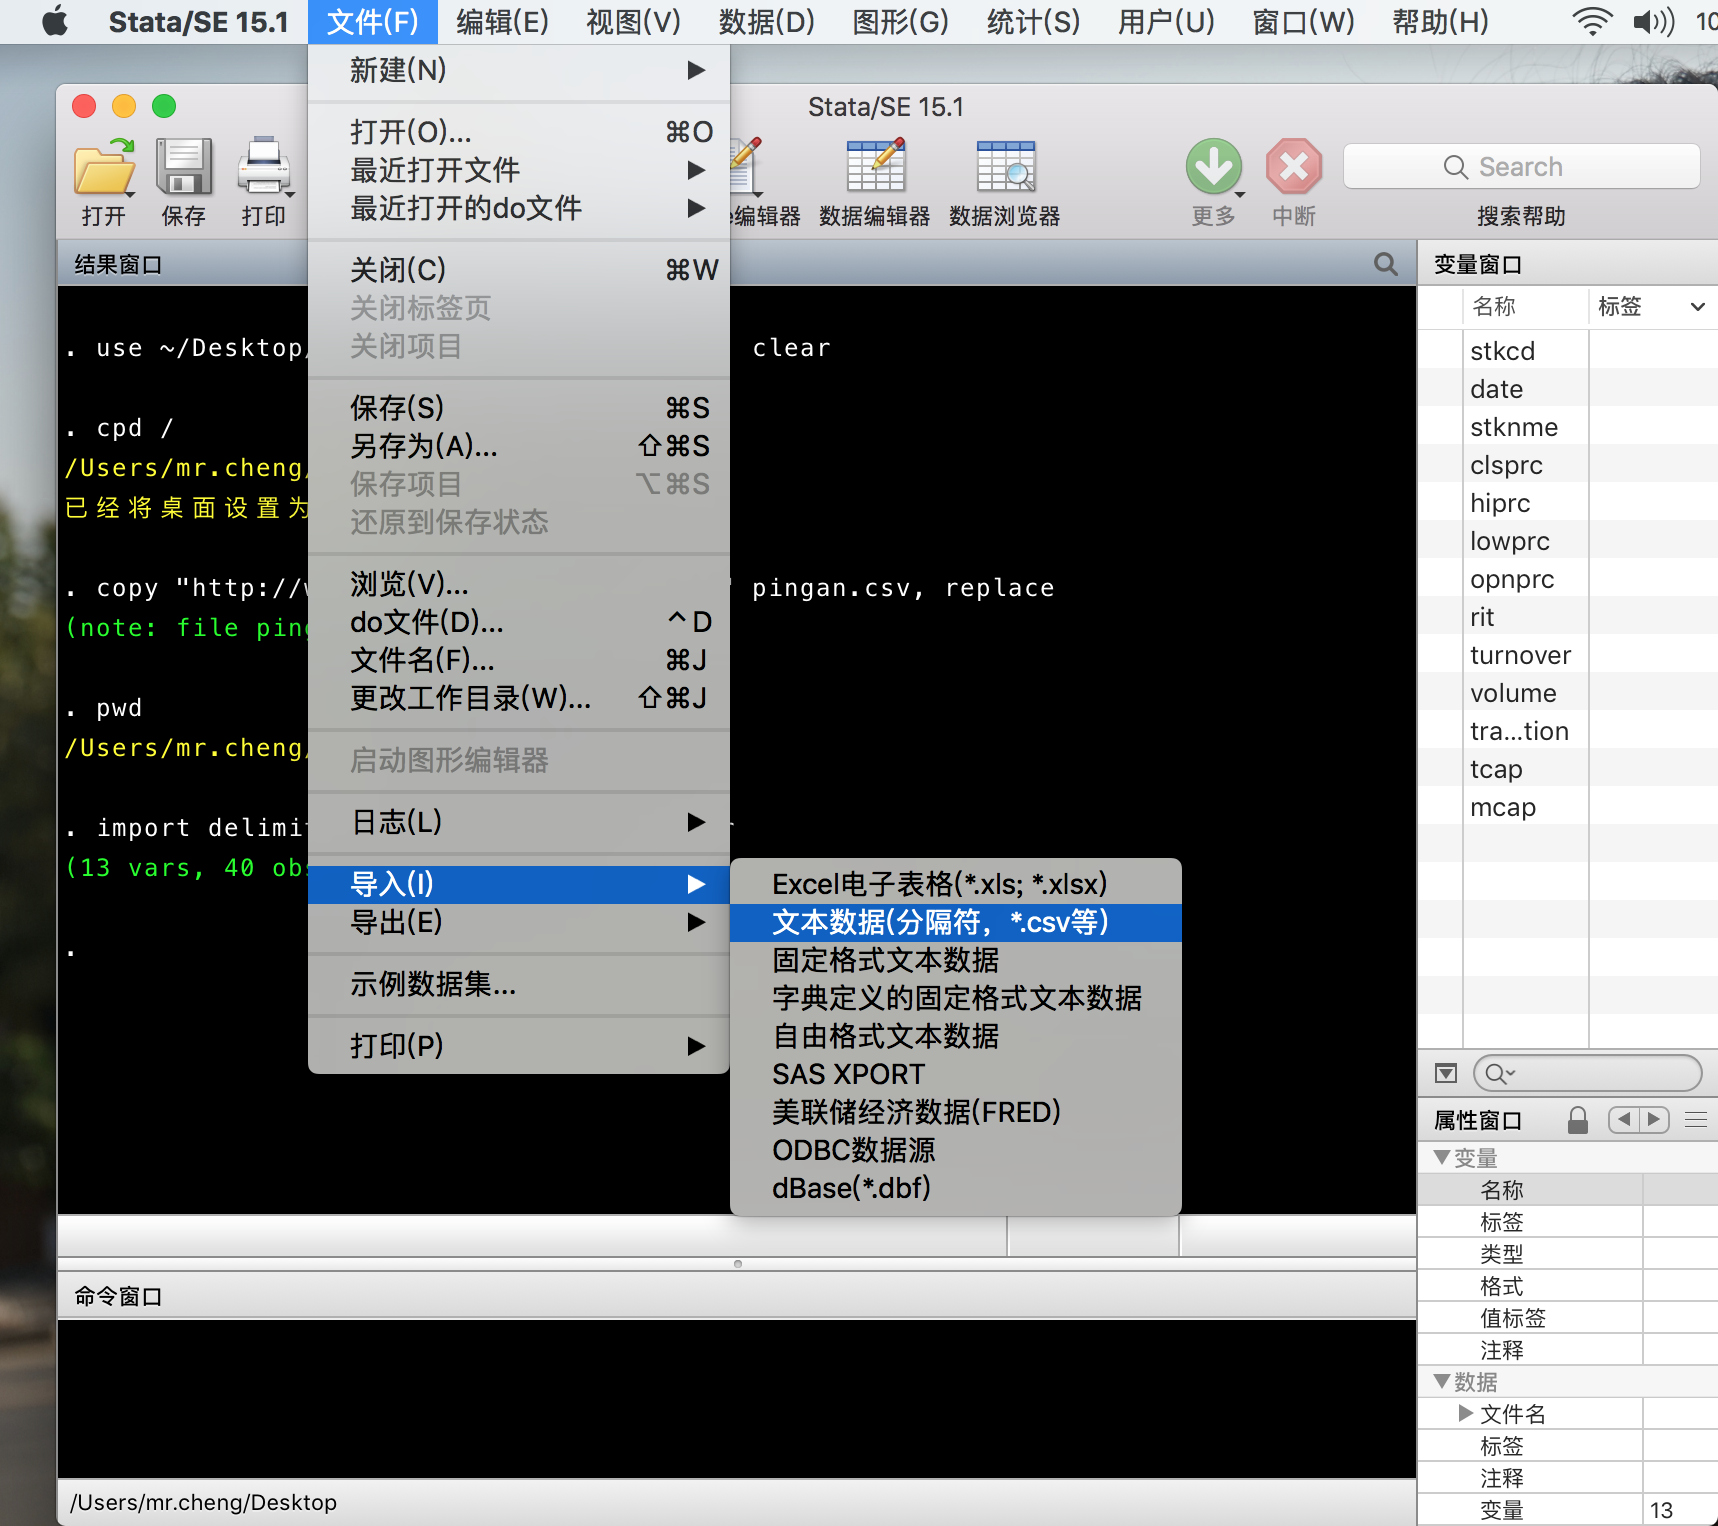
\includegraphics[width=0.9\textwidth]{assets/csvgui1.png}
  \caption{Stata 通过 GUI 导入 csv 数据(1)}
  \label{fig:csvgui1}
\end{figure}

稍等片刻,在对话框里进行选择,然后提交即可:

\begin{figure}[htbp]
  \centering 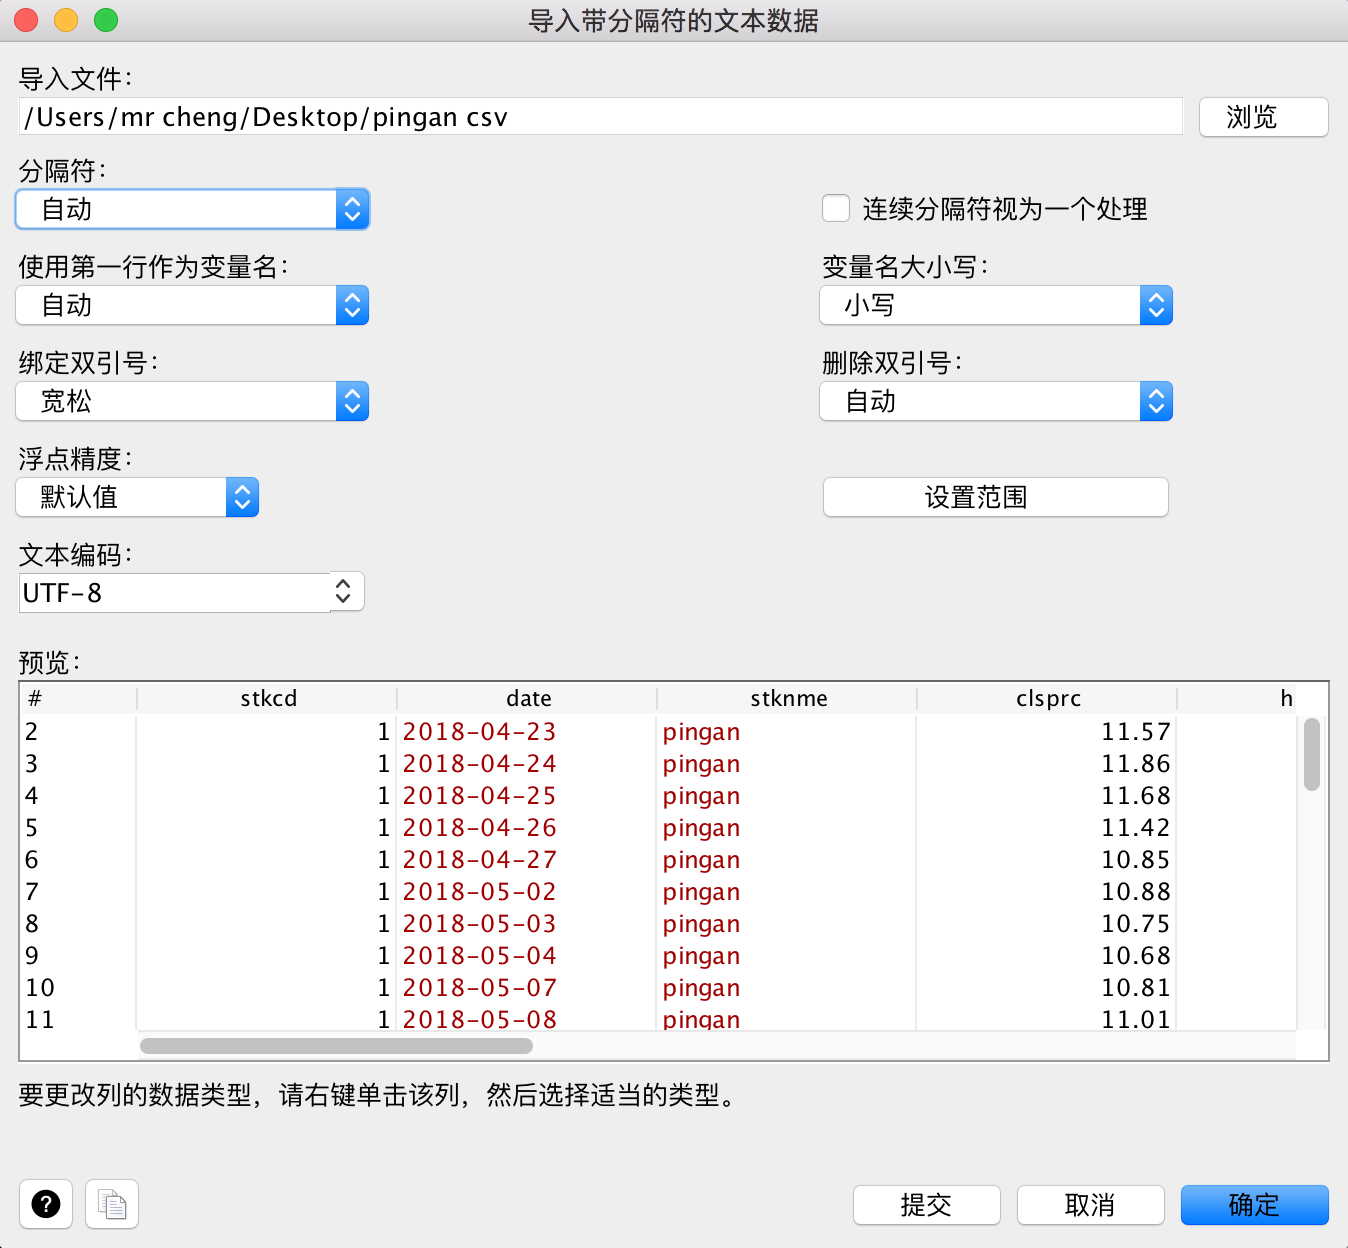
\includegraphics[width=0.7\textwidth]{assets/csvgui2.png}
  \caption{Stata 通过 GUI 导入 csv 数据(2)}
  \label{fig:csvgui2}
\end{figure}

为了保存这个操作,我们最好把这个提交动作的命令复制粘贴到我们的do文档里面:

\begin{lstlisting}
import delimited /Users/czx/Desktop/pingan.csv, ///
    delimiter(comma) varnames(1) encoding(utf8) clear
\end{lstlisting}

\subsection{读入xls、xlsx数据}

这两种格式的数据是 Excel 的数据,例如我想导入 \texttt{grilic\_small.xls} 数据集:

\begin{lstlisting}
* 首先用copy下载:
copy "https://czxb.github.io/mr/grilic_small.xls" grilic_small.xls, replace
import excel using grilic_small.xls, clear firstrow
\end{lstlisting}

\texttt{firstrow} 表示设定第一行为变量名。

同样导入 Excel 文件也能通过界面鼠标点击操作。

\subsection{导入自由格式的txt文件}

下面我要介绍的这种是在使用Stata爬数据的时候最为常用的一种方法了。

假如我想爬东方财富网的采购经理人指数:网址是:\href{http://data.eastmoney.com/cjsj/pmi.html}{中国 采购经理人指数(PMI)}。那么第一步就是我的把这个网页读入Stata,下面的命令就可以实现了:

\begin{lstlisting}
* 首先把这个网页下载存储为temp.txt文件:
copy "http://data.eastmoney.com/cjsj/pmi.html" temp.txt, replace
* 然后读入Stata,把每一行的前20000个字符(可以确定是整行了)读入strL格式的变量v。
infix strL v 1-20000 using temp.txt, clear
\end{lstlisting}

然后你会发现这个变量v里面的有些观测值是乱码的,这是因为这个网页文件不是 \texttt{UTF-8} 编码的,所以需要先把这个 \texttt{temp.txt} 文件转一下码。 Stata 中的转码命令是:

\begin{lstlisting}
unicode encoding set gb18030
unicode translate 文件名.后缀名
unicode erasebackups, badidea
\end{lstlisting}

所以我们把这个temp.txt文件转个码再读如Stata中:

\begin{lstlisting}
* 首先清空内存,这个清空是非常彻底的清空。
clear all
copy "http://data.eastmoney.com/cjsj/pmi.html" temp.txt, replace
unicode encoding set gb18030
unicode translate temp.txt
unicode erasebackups, badidea
infix strL v 1-20000 using temp.txt, clear
\end{lstlisting}

然后就会发现乱码问题得到了解决。
Stata14之前的版本创建的数据集读入Stata14、15都是需要转码的,都可以用这三句命令完成。

但是每次都打这三句是不是非常麻烦?所以我简单把这三句封装成了一个小命令\texttt{utrans}。
这个命令位于我的finance命令包中,安装finance包即可安装这个命令:

\begin{lstlisting}
github install czxa/finance, replace
\end{lstlisting}

然后上面的转码只需要\texttt{utrans\ +\ 文件即可完成}:

\begin{lstlisting}
utrans temp.txt
*> 转码完成
\end{lstlisting}

\section{数据处理}

当我们把数据读入之后就能进行数据处理了。数据处理的熟练程度直接决定了你写论文的速度。这里介绍一些常用的Stata处理数据的命令。

\subsection{describe:审视数据}

这个命令可以被简写为\texttt{des}。建议初学者不要立即使用简写,以免后来记不住命令的全称。

\begin{lstlisting}
sysuse auto, clear
*> (1978 Automobile Data)

des
*> Contains data from /Applications/Stata/ado/base/a/auto.dta
*>   obs:            74                          1978 Automobile Data
*>  vars:            12                          13 Apr 2016 17:45
*>  size:         3,182                          (_dta has notes)
*> ----------------------------------------------------------------------
*>               storage   display    value
*> variable name   type    format     label      variable label
*> ----------------------------------------------------------------------
*> make            str18   %-18s                 Make and Model
*> price           int     %8.0gc                Price
*> mpg             int     %8.0g                 Mileage (mpg)
*> rep78           int     %8.0g                 Repair Record 1978
*> headroom        float   %6.1f                 Headroom (in.)
*> trunk           int     %8.0g                 Trunk space (cu. ft.)
*> weight          int     %8.0gc                Weight (lbs.)
*> length          int     %8.0g                 Length (in.)
*> turn            int     %8.0g                 Turn Circle (ft.)
*> displacement    int     %8.0g                 Displacement (cu. in.)
*> gear_ratio      float   %6.2f                 Gear Ratio
*> foreign         byte    %8.0g      origin     Car type
*> ----------------------------------------------------------------------
*> Sorted by: foreign
\end{lstlisting}

\subsection{list:列示数据}

这个命令有两种用法,第一种是列示某些变量,第二种是列示某些观测值:

\begin{lstlisting}
/* 列示整个数据表 */
list

/* 列示变量price和make */
list price make

/* 列示所有变量的第5-10个观测值 */
list in 5/10

/* 列示变量price和make的最后一个观测值 */
list price make in -1

/* 列示price大于10000的部分 */
list price if price > 10000
\end{lstlisting}

\subsection{gsort/order:排序}

sort命令正在被逐渐弃用。gsort用于观测值的排序,order用于变量的排序。

\begin{lstlisting}
/* 把price按照由低到高的顺序排列 */
gsort price

/* 把price按照由高到低的顺序排列 */
gsort -price

/* 先排rep78再排price */
gsort rep78 -price
\end{lstlisting}

\subsection{codebook:描述变量的基本信息}

\begin{lstlisting}
codebook
codebook price
*> --------------------------------------------------------------------------
*> price                                                               Price
*> --------------------------------------------------------------------------
*>
*>                   type:  numeric (int)
*>
*>                  range:  [3291,15906]                 units:  1
*>          unique values:  74                       missing .:  0/74
*>
*>                   mean:   6165.26
*>               std. dev:    2949.5
*>
*>            percentiles:        10%       25%       50%       75%       90%
*>                               3895      4195    5006.5      6342     11385
\end{lstlisting}

从上面的结果中可以看到:

\begin{enumerate}
\item price 变量为数值型变量;
\item 范围在 {[}3291,15906{]};
\item 有74个观测值,互不相同且没有缺失值;
\item 均值为6165.26,标准差为2949.5;
\item 分位数看起来是合理的。
\end{enumerate}

\subsection{generate:生成新变量}
这个命令可以简写为\texttt{gen}。

\begin{lstlisting}
/* 例如我想生成一列等于观测值编号的变量v */
gen v = _n

/* 再例如我想生成一列等于总观测值数据的变量v1 */
gen v1 = _N

/* 还可以和数学函数一起使用,例如生成pirce的平方序列 */
gen price2 = price^2
\end{lstlisting}

gen还可以和by/bysort一起使用。例如我想生成一个表示rep78变量的每个值的个数的变量v2:

\begin{lstlisting}
bysort rep78: gen v2 = _N
* 或者
bysort rep78: egen v3 = count(mpg)
\end{lstlisting}

\subsection{replace: 替换}

\begin{lstlisting}
/* 例如把rep78中的缺失值都替换成0(Stata中的数值型变量的缺失值用点表示,其实际数值是无穷大) */
replace rep78 = 0 if rep78 == .

/* 或者 */
replace rep78 = 0 if missing(rep78)

/* 把 price 变量取值在 10000-15000 的观测值替换成-1 */
replace price = -1 if inrange(price, 10000, 15000)

/* 把 make 变量取值为 "Olds Starfire" 和 "Dodge St. Regis" 的替换成 "" (空字符串) */
replace make = "" if inlist(make, "Olds Starfire", "Dodge St. Regis")

/* 把 make 变量中含字母A的观测值替换成空字符串 */
replace make = "" if index(make, "A")
\end{lstlisting}

\subsection{rename:重命名变量}

这个命令可以简写为ren。

\begin{lstlisting}
/* 例如把 make 重命名为 make1 */
ren make make1
\end{lstlisting}

\subsection{drop:删除}

这个命令也有两种用法:删除变量和删除观测值。

\begin{lstlisting}
/* 删除变量make1 */
drop make1

/* 删除第5-10个观测值 */
drop in 5/10

/* 删除price大于10000的观测值 */
drop if price > 10000

/* 使用通配符:删除m开头的变量 */
drop m*
\end{lstlisting}

\subsection{summarize:查看描述性统计量}

这个命令可以简写为 sum :

\begin{lstlisting}
sum price
sum price if price > 10000
sum price, detail
\end{lstlisting}

\subsection{tabulate:查看频率频数表}

这个命令可以被简写为 tab:

\begin{lstlisting}
tab rep78
\end{lstlisting}

\subsection{pwcorr:计算相关系数表}

\begin{lstlisting}
pwcorr price length weight, star(0.05) sig
\end{lstlisting}

\begin{itemize}
\item  star 表示在5\%显著性水平上显著的相关系数上标星星。
\item  sig 表示显示显著性水平。
\end{itemize}

corr 命令也能用于计算相关系数表:

\begin{lstlisting}
corr price weight

/* 还可以用来计算协方差矩阵 */
corr price weight, c
\end{lstlisting}

\subsection{display}

这个命令可以被简写为\texttt{di},用于打印:

\begin{lstlisting}
display "这是一行字符串"
di as text "这是一行字符串"
di as error "这是一行字符串"
di as result "这是一行字符串"
di in green "这是一行字符串"
di in red "这是一行字符串"
di in yellow "这是一行字符串"
di in white "这是一行字符串"
di as input di in white "这是一行字符串"
di 3 + 4
di 2^0.5

sysuse auto, clear
*> (1978 Automobile Data)

summarize mpg
*>
*>     Variable |        Obs        Mean    Std. Dev.       Min        Max
*> -------------+---------------------------------------------------------
*>          mpg |         74     21.2973    5.785503         12         41
*>

di as text "mean of mpg = " as result r(mean)
*> mean of mpg = 21.297297
\end{lstlisting}

\section{数据导出}
\subsection{save: 导出为dta文件}

\begin{lstlisting}
save auto2, replace
\end{lstlisting}

\subsection{export delimited:导出为csv文件}

\begin{lstlisting}
export delimited using auto2.csv, replace
\end{lstlisting}

\subsection{export excel:导出为excel文件}

\begin{lstlisting}
export excel using auto2.xlsx, replace
\end{lstlisting}

\section{绘图}
\subsection{histogram:绘制直方图}

这个命令可以被简写为hist:

\begin{lstlisting}
cuse grilic_small, c w
hist s, width(1) freq
\end{lstlisting}

\begin{itemize}
\item  width:组宽
\item  freq:设定纵轴为频数,默认是密度
\end{itemize}

\begin{figure}[htbp]
  \centering
  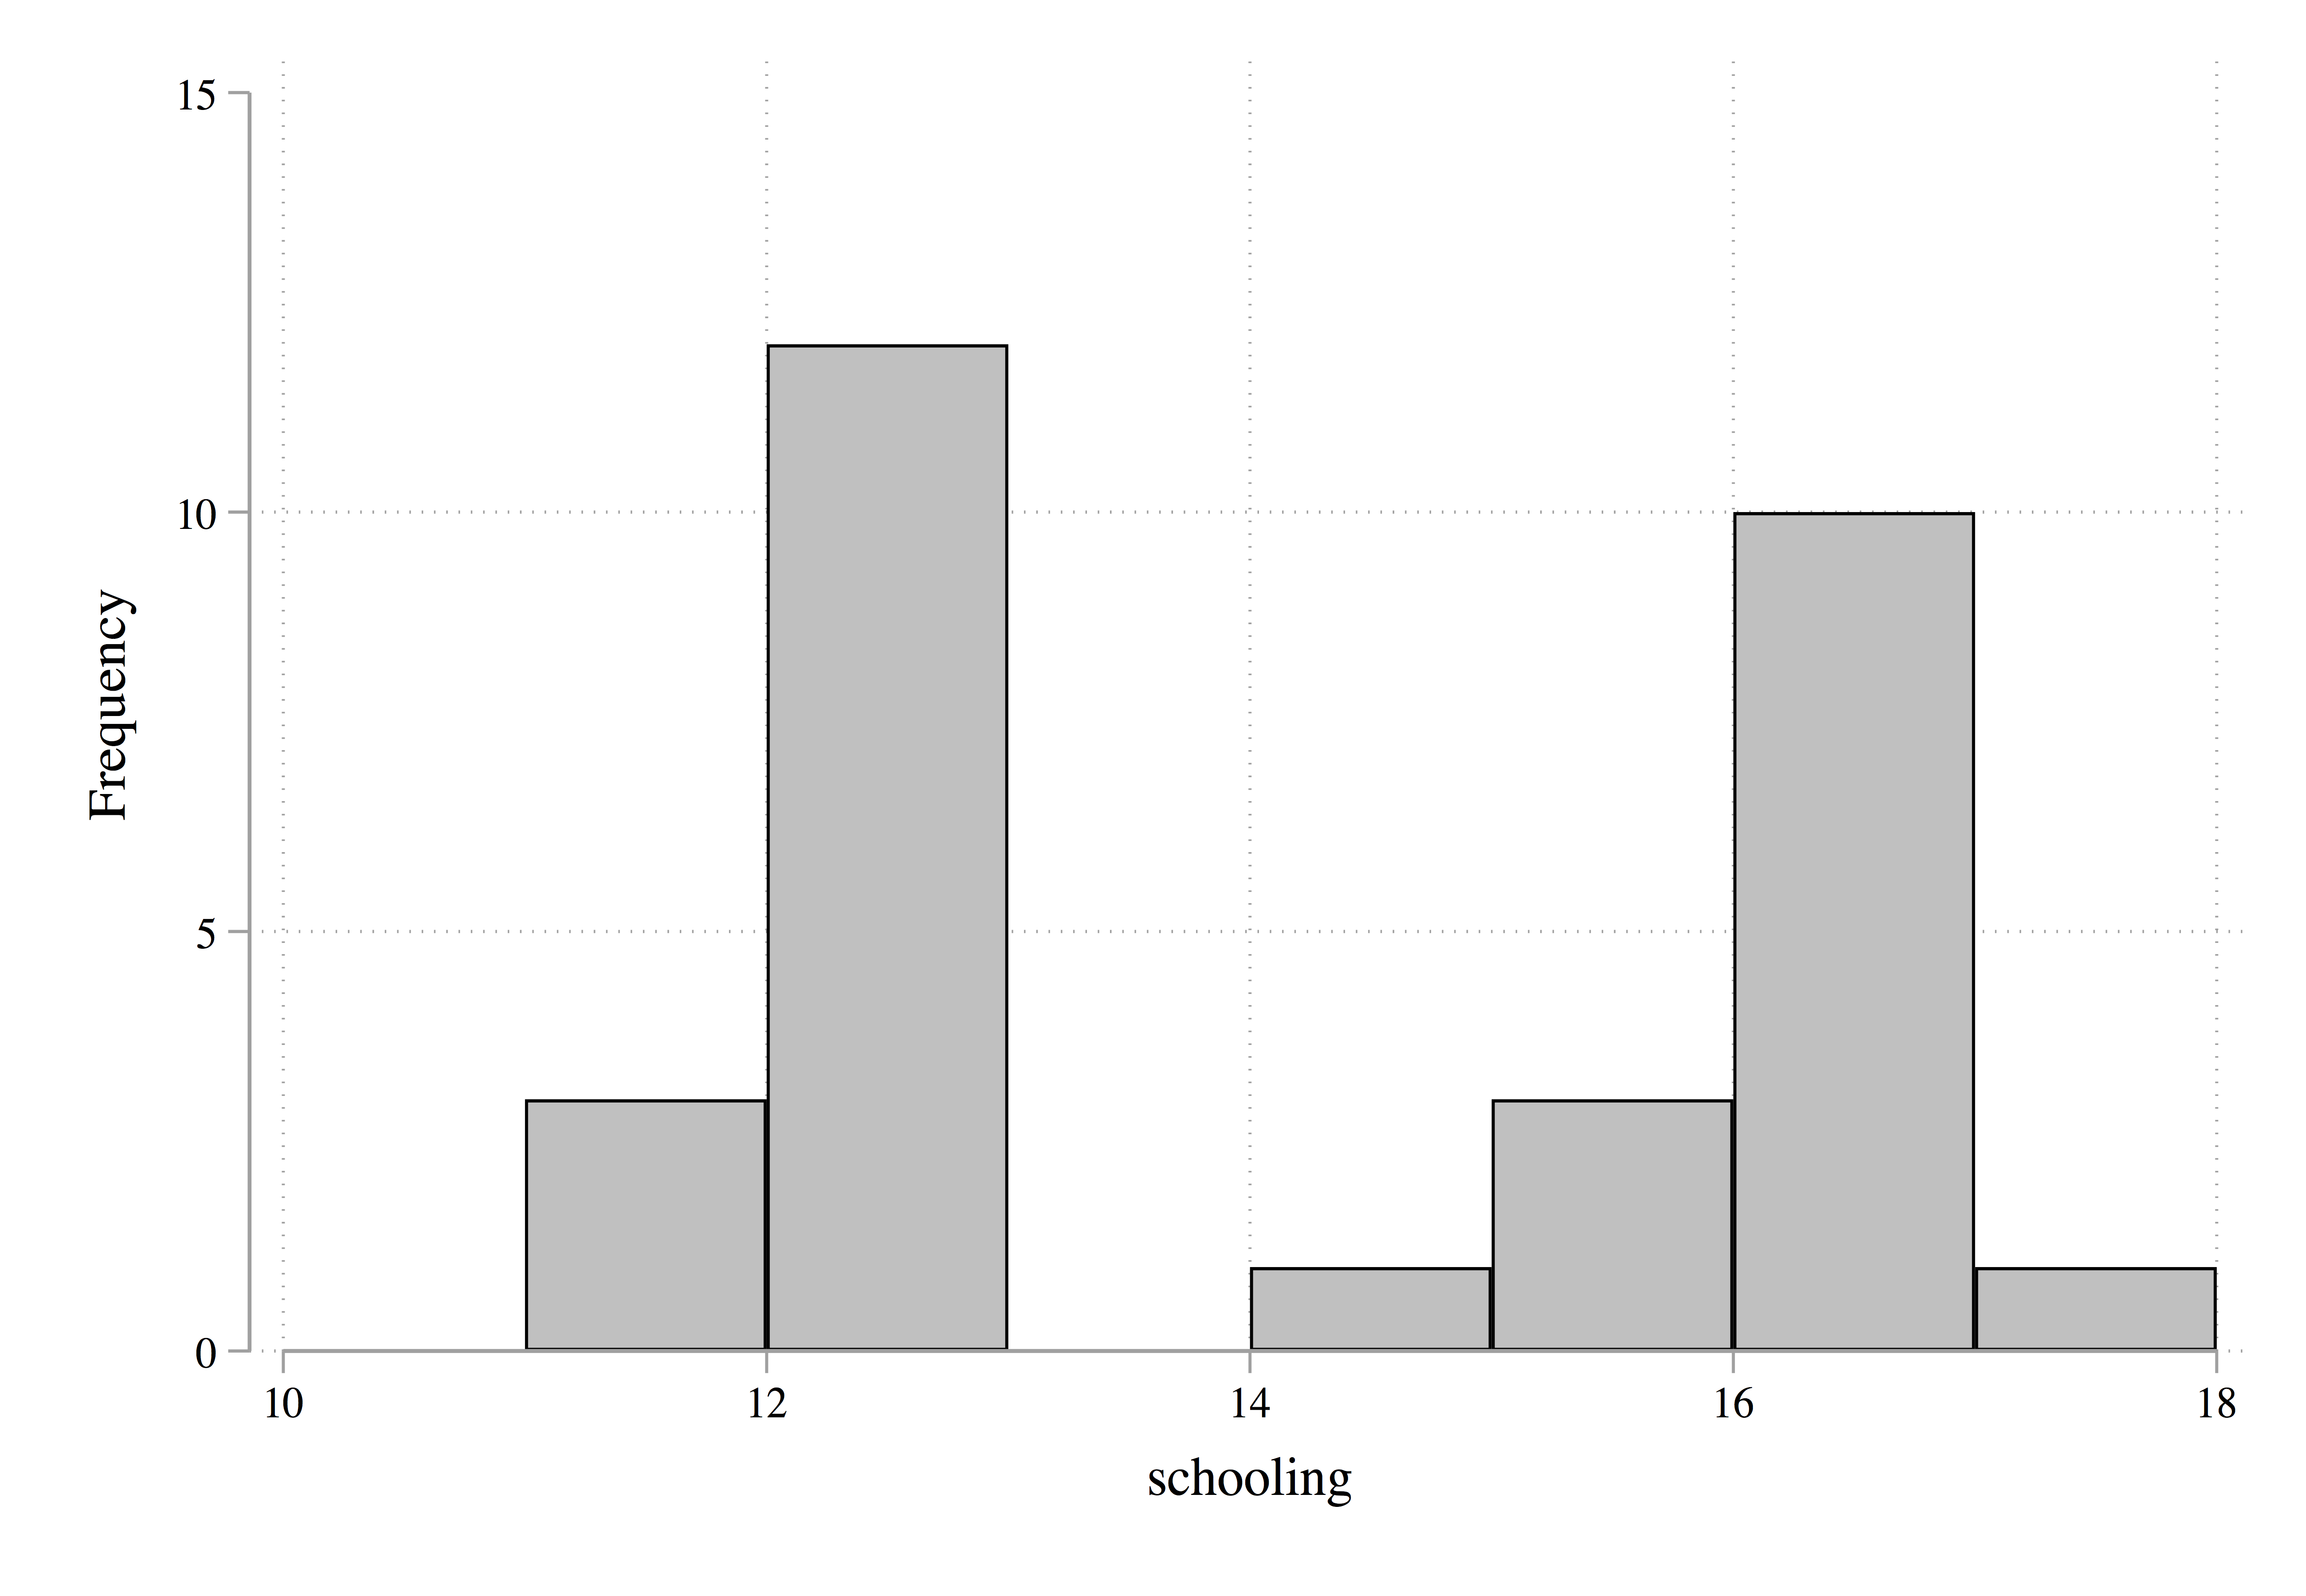
\includegraphics[width=\textwidth]{assets/hist.png}
  \caption{直方图}
  \label{fig:hist}
\end{figure}

\begin{remark}
推荐大家使用plotplain主题,刚刚安装 finance 命令包的时候这个主题已经安装好了,使用 scheme() 选项可以指定选项。
\end{remark}

\begin{lstlisting}
hist s, width(1) freq sch(plotplain)
\end{lstlisting}

\subsection{scatter:绘制散点图}

\begin{lstlisting}
/* 例如,我想观察工资和受教育年限之间的关系 */
gen n = _n
sc lnw s, mlab(n) msize(*2) mc(red*0.6) xti("受教育年限") yti("对数工资")
\end{lstlisting}

\begin{figure}[htbp]
  \centering 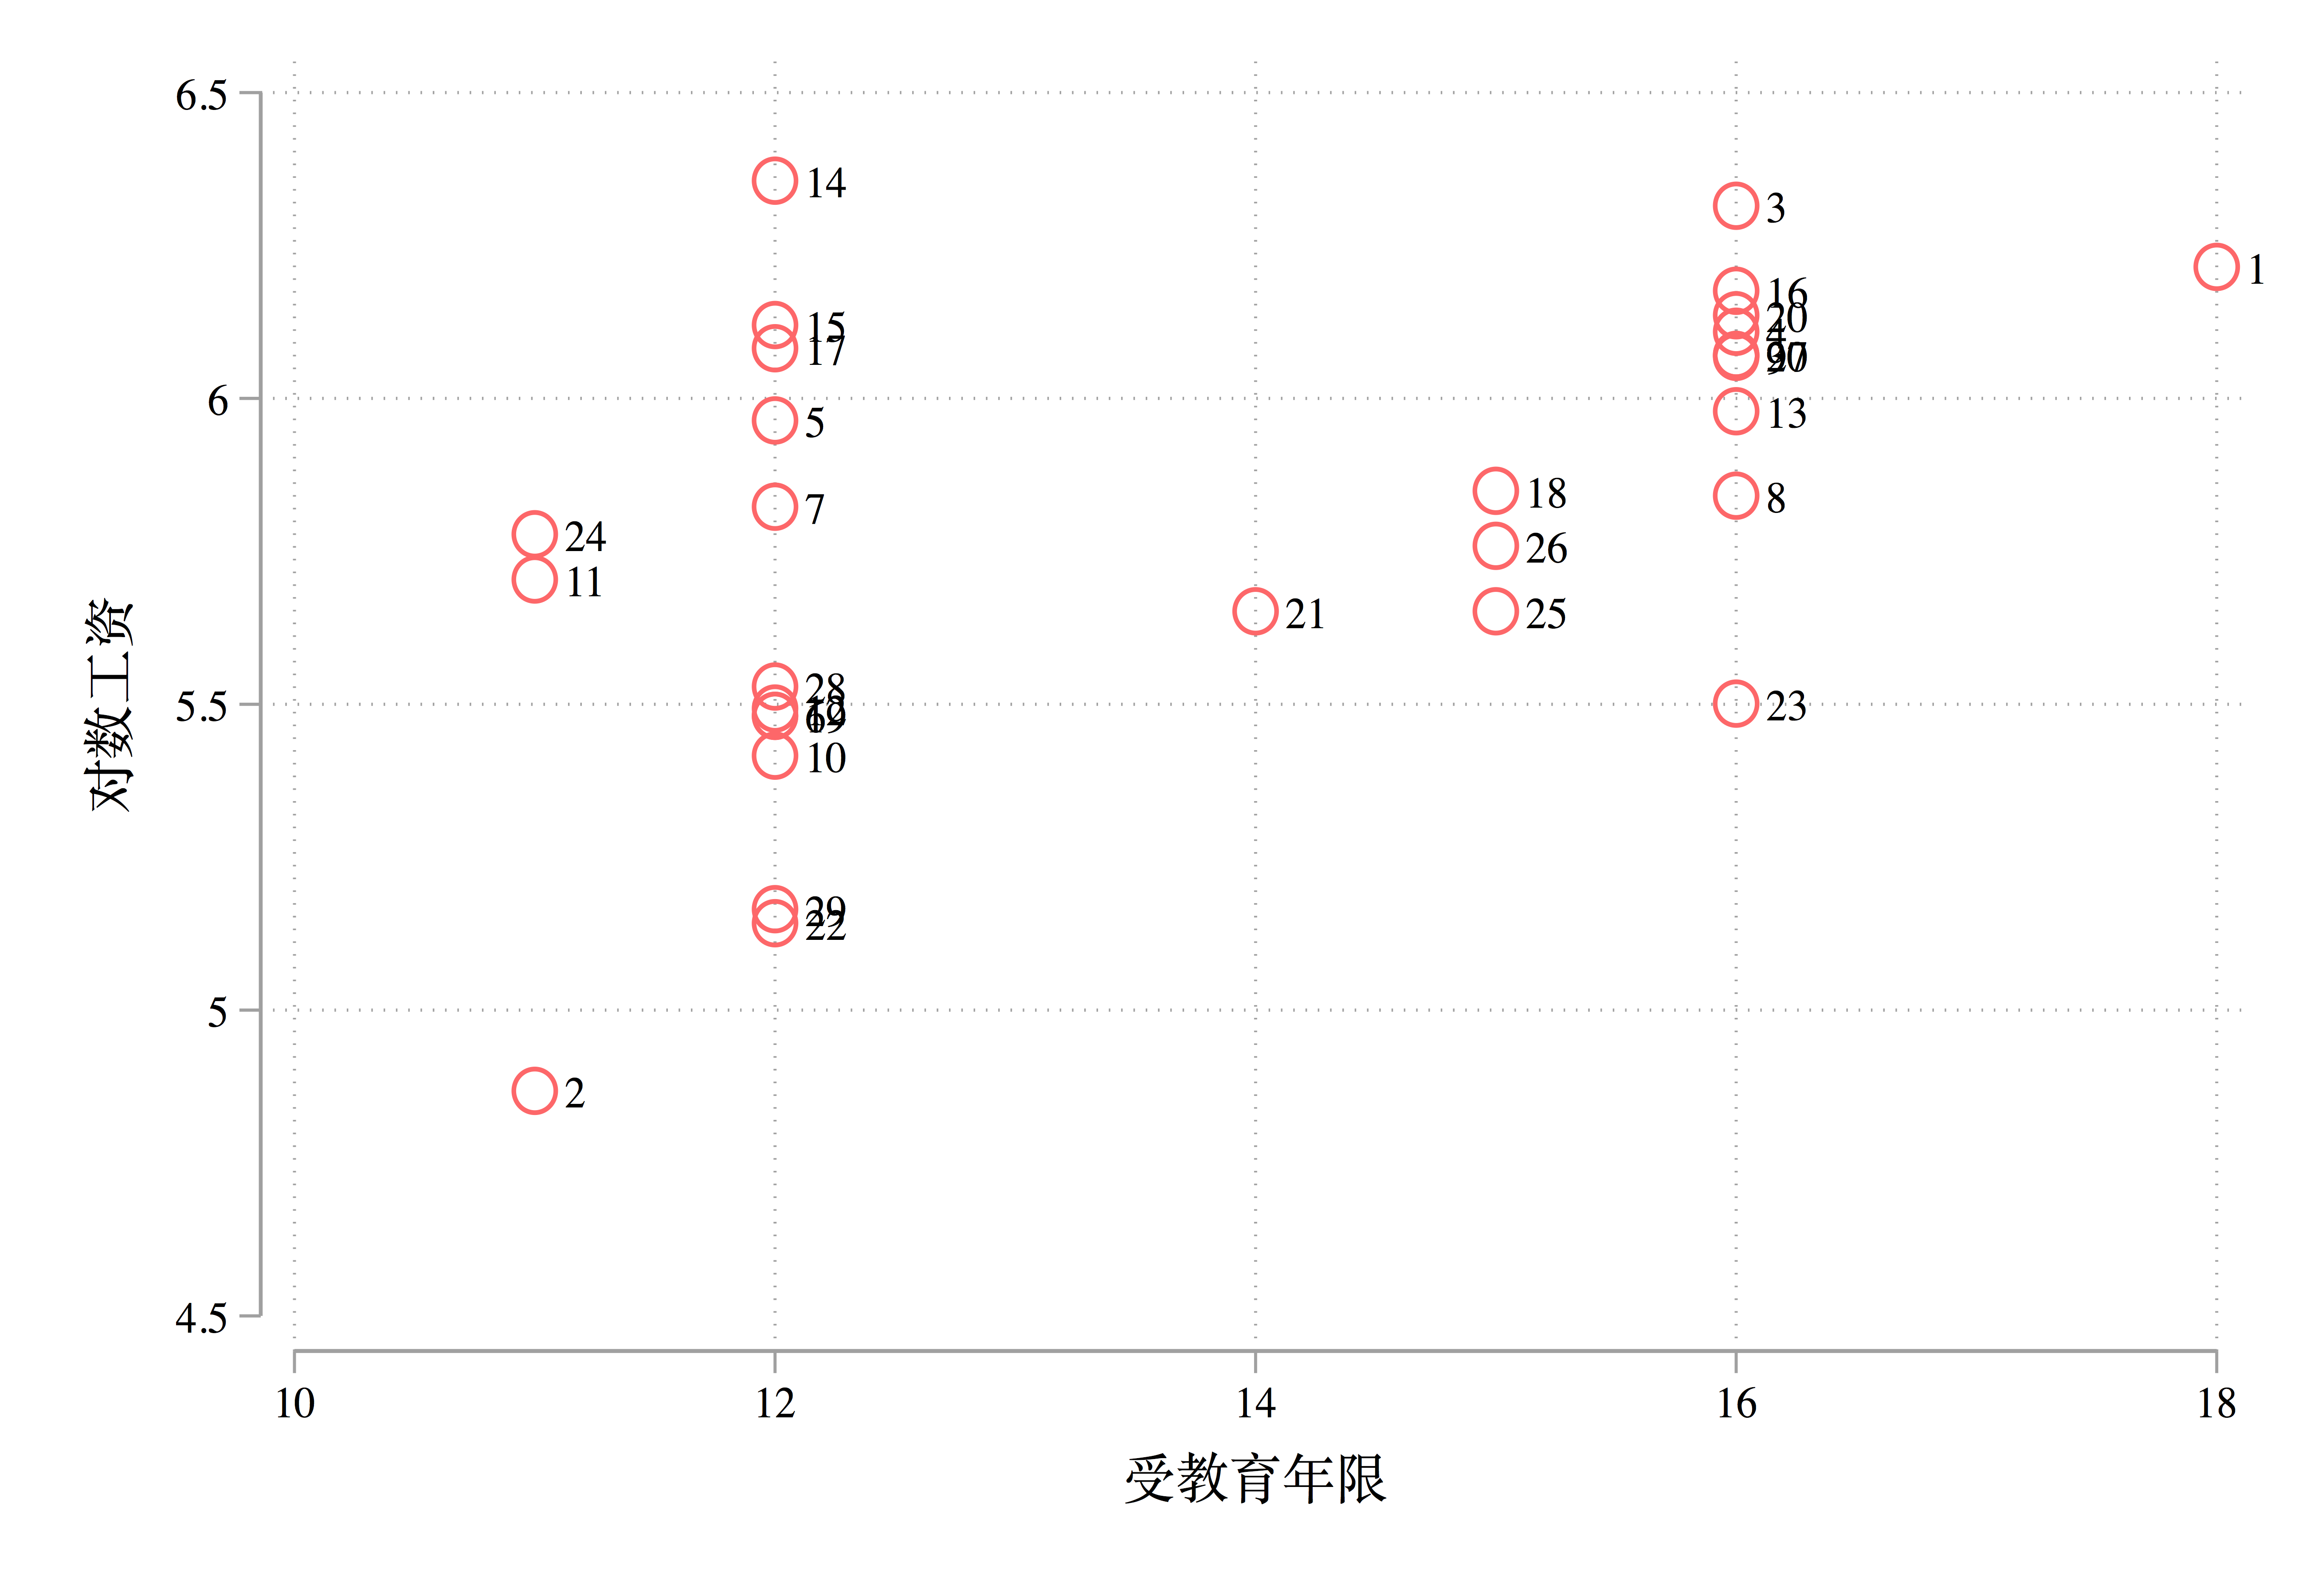
\includegraphics[width=\textwidth]{assets/scatter.png}
  \caption{散点图}
  \label{fig:scatter}
\end{figure}

\section{统计相关}
\subsection{grilic数据集示例}
\begin{lstlisting}
cuse grilic, c w
ren lw lnw
des
sum
sum lnw, d
hist lnw, width(0.1)
kdensity lnw, normal normop(lp(dash)) leg(pos(6) row(1)) ///
  xti("工资对数") yti("密度") ///
  yla(,format(%6.1f))
\end{lstlisting}

\begin{figure}[htbp]
  \centering 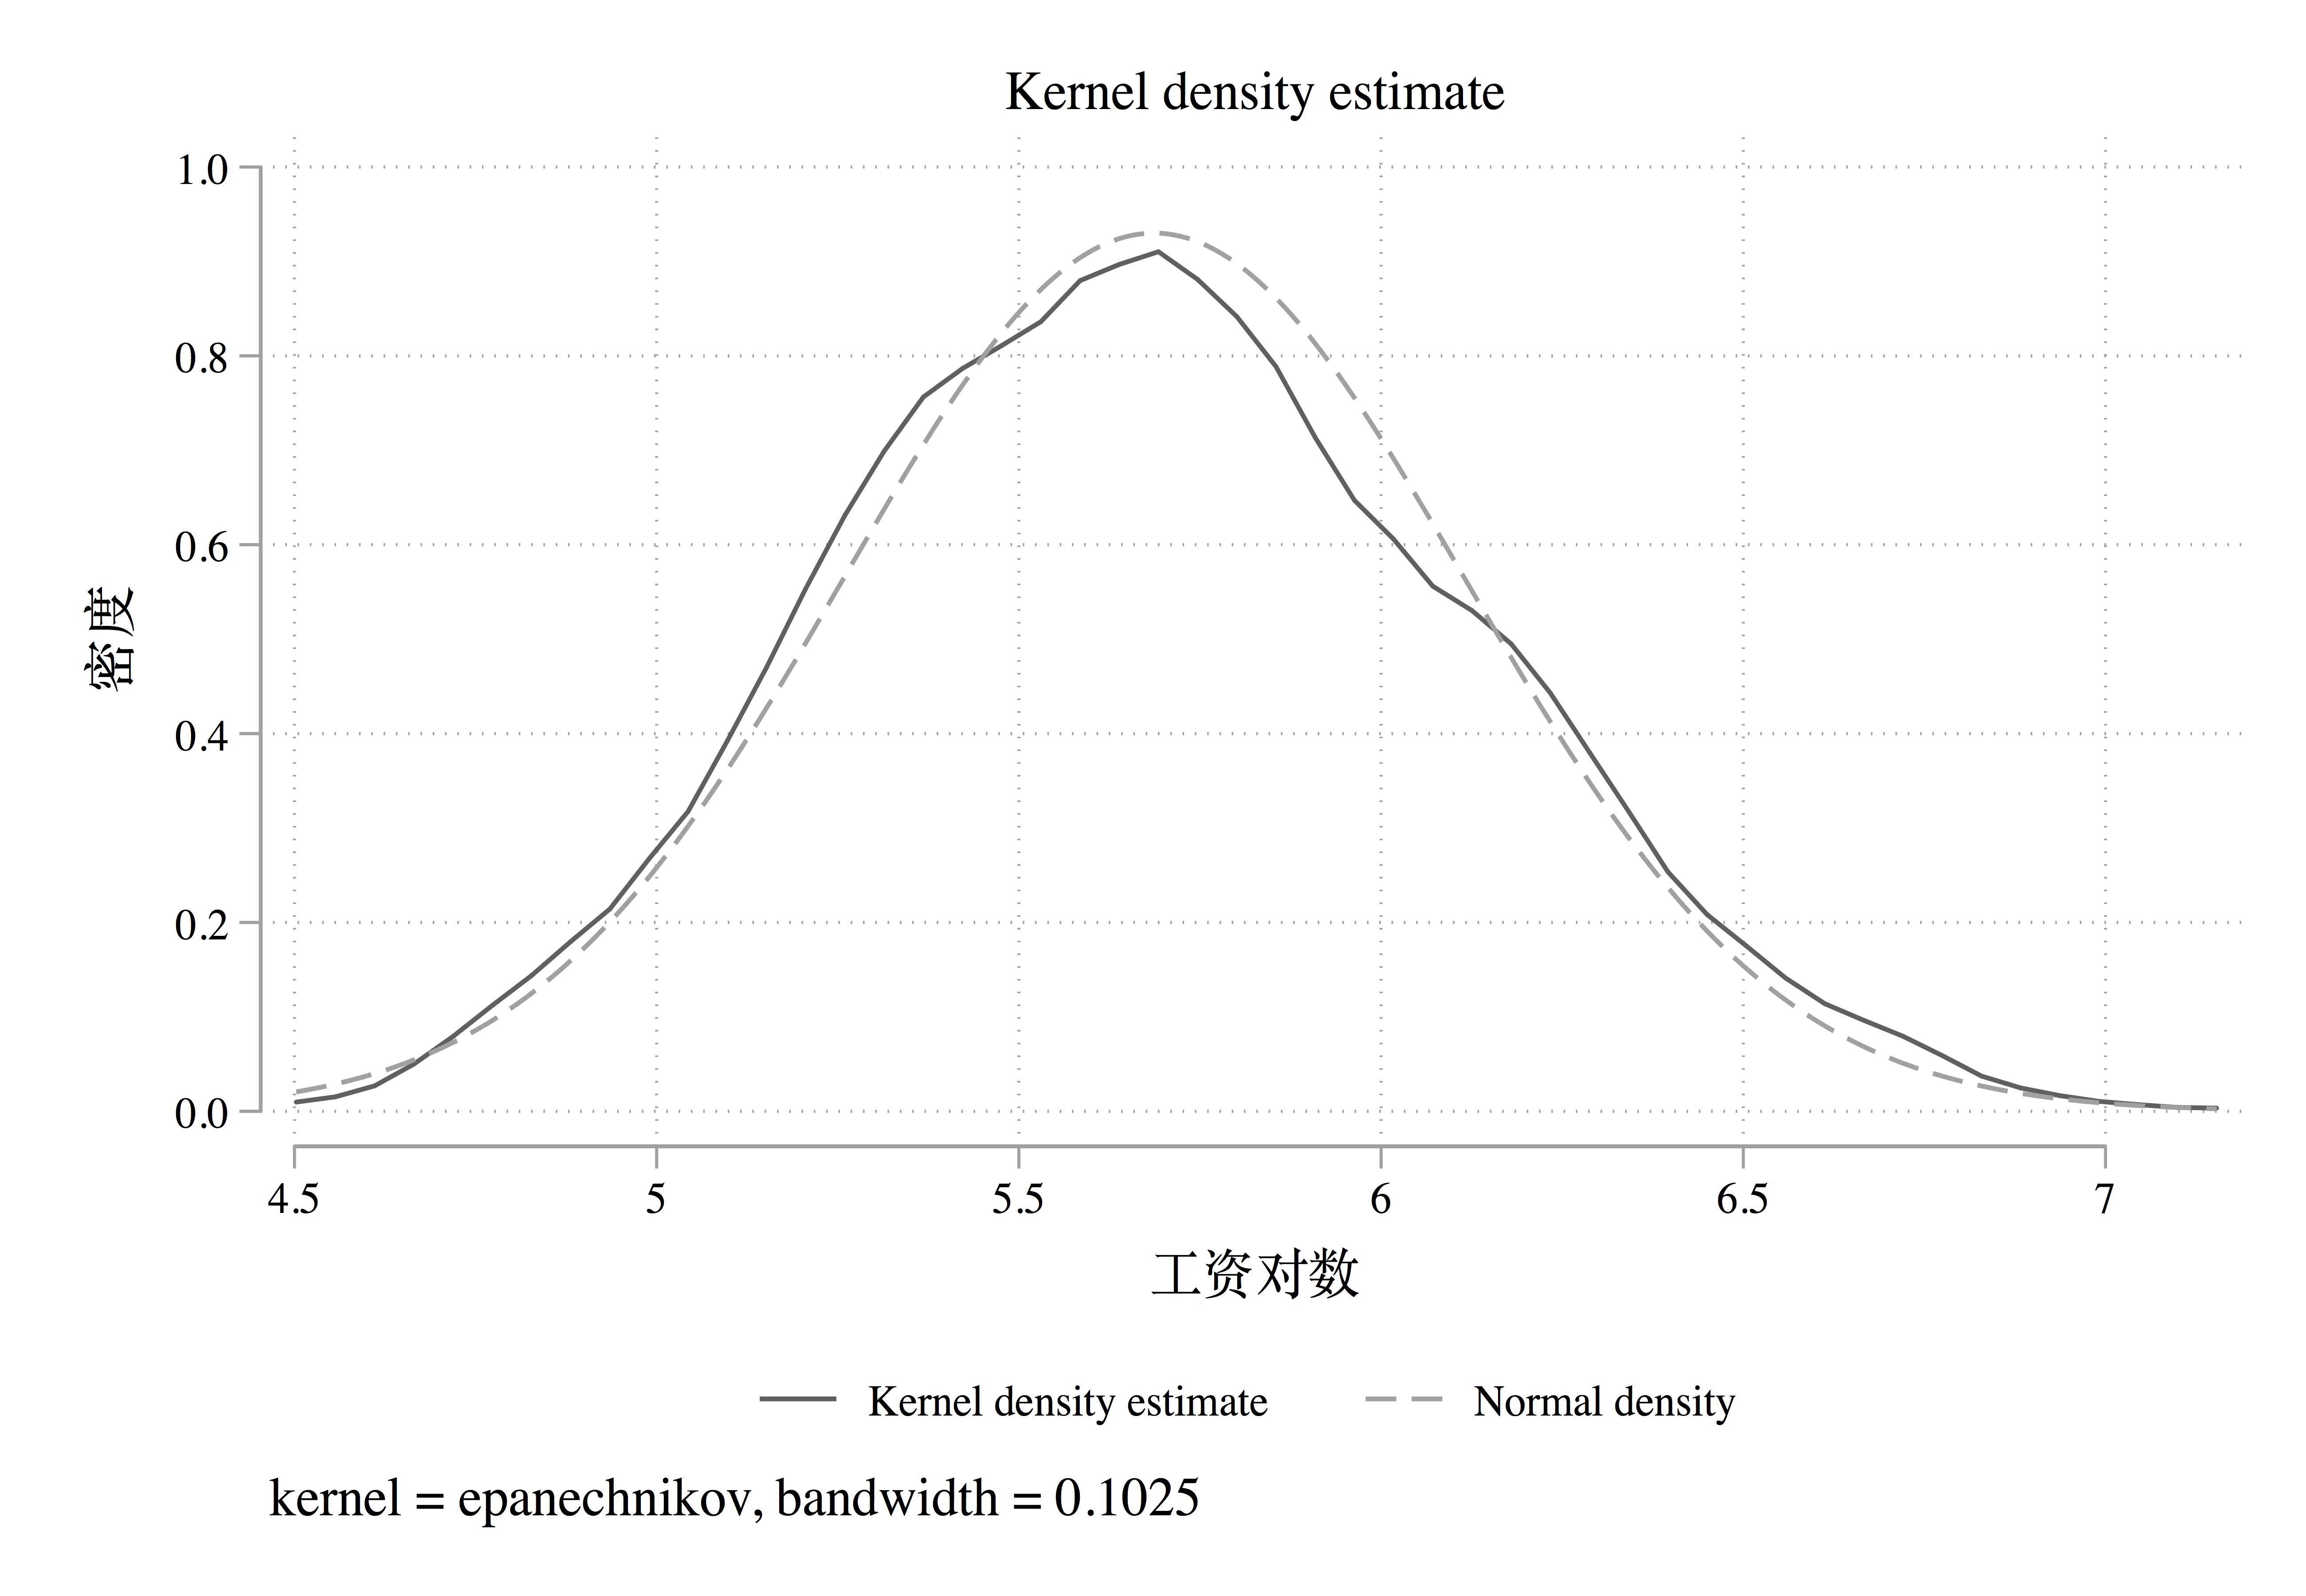
\includegraphics[width=\textwidth]{assets/kden.png}
  \caption{工资对数的核密度估计图}\label{fig:kden}
\end{figure}

\begin{lstlisting}
tw ///
kdensity lnw || ///
kdensity lnw if s == 16, lp(dash) ||, ///
    xti("工资对数") yti("密度") ///
    leg(pos(6) row(1)) ///
    yla(#4, format(%6.1f)) xla(, format(%6.1f)) ///
\end{lstlisting}

\begin{figure}[htbp]
  \centering 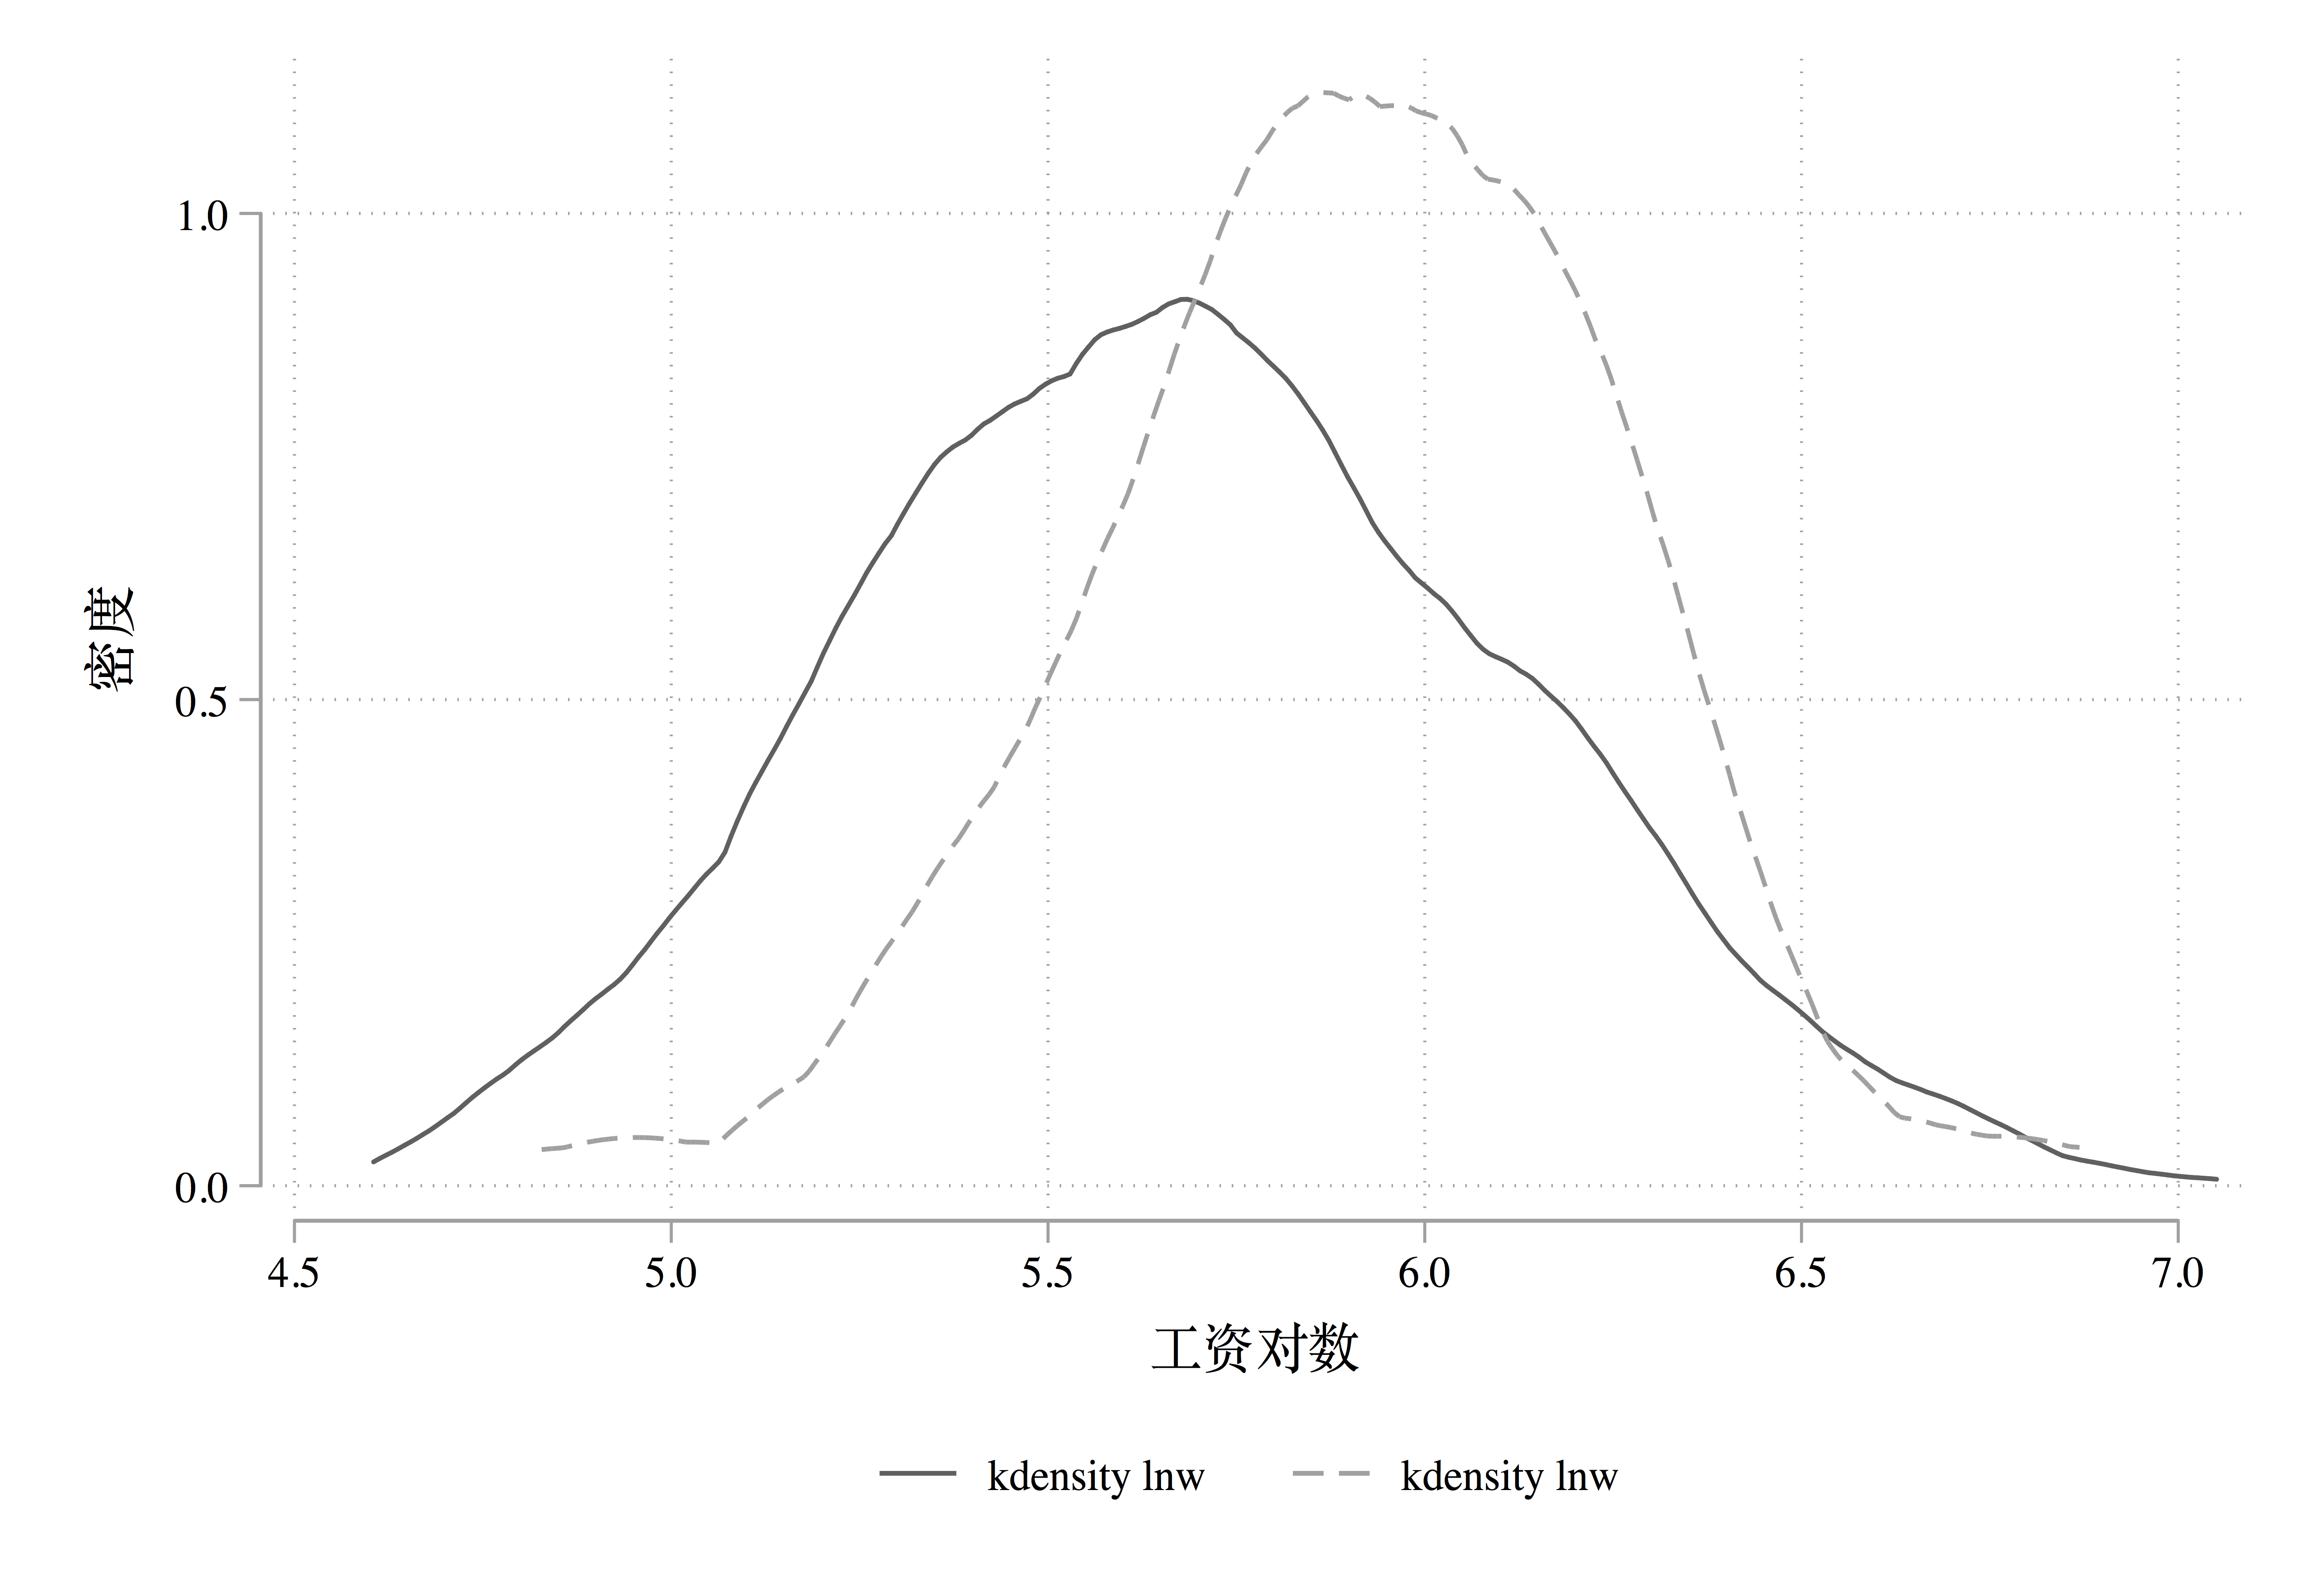
\includegraphics[width=\textwidth]{assets/kdensity2.png}
  \caption{工资对数的核密度估计图与受教育年限为16年的样本工资对数和密度估计图}
  \label{fig:kden2}
\end{figure}

\subsection{验证迭代期望定律}

\begin{definition}{迭代期望定律}{expectation}
  \begin{equation}
    E(Y) = E_x[E(Y|x)]
  \end{equation}
\end{definition}

使用数据集grilic.dta来验证该定律:

\[E(lnw) = E_{rns} \times [E(lnw|rns)]\]

\begin{itemize}
\item  rns是一个虚拟变量,首先我们计算 \texttt{{[}E(lnw\textbar{}rns=1){]}} 和 \texttt{{[}E(lnw\textbar{}rns=0){]}}
\item  那么 \texttt{E\_rns{[}E(lnw\textbar{}rns){]}} 等于两者的加权平均:
\item  先别急着算,均值这么长,抄起来多累,我们重新开始,这一次使用宏变量来记录每一次的均值。
\end{itemize}

\begin{lstlisting}
cuse grilic, c w
ren lw lnw
sum lnw if rns == 1
return list
local a = r(mean)
sum lnw if rns == 0
return list
local b = r(mean)
di (`a'*204+`b'*554)/(204+554)
*> 5.6867388
\end{lstlisting}

另一方面,E(lnw)为:

\begin{lstlisting}
sum lnw
    Variable |        Obs        Mean    Std. Dev.       Min        Max
-------------+---------------------------------------------------------
         lnw |        758    5.686739    .4289494      4.605      7.051
\end{lstlisting}

忽略舍入误差,两者完全相等。从而得证。

\chapter{数据可视化}

本书第一部分的目标是让你尽快掌握数据探索的基本工具。数据分析的流程大致如下:

\begin{figure}[htbp]
  \centering
  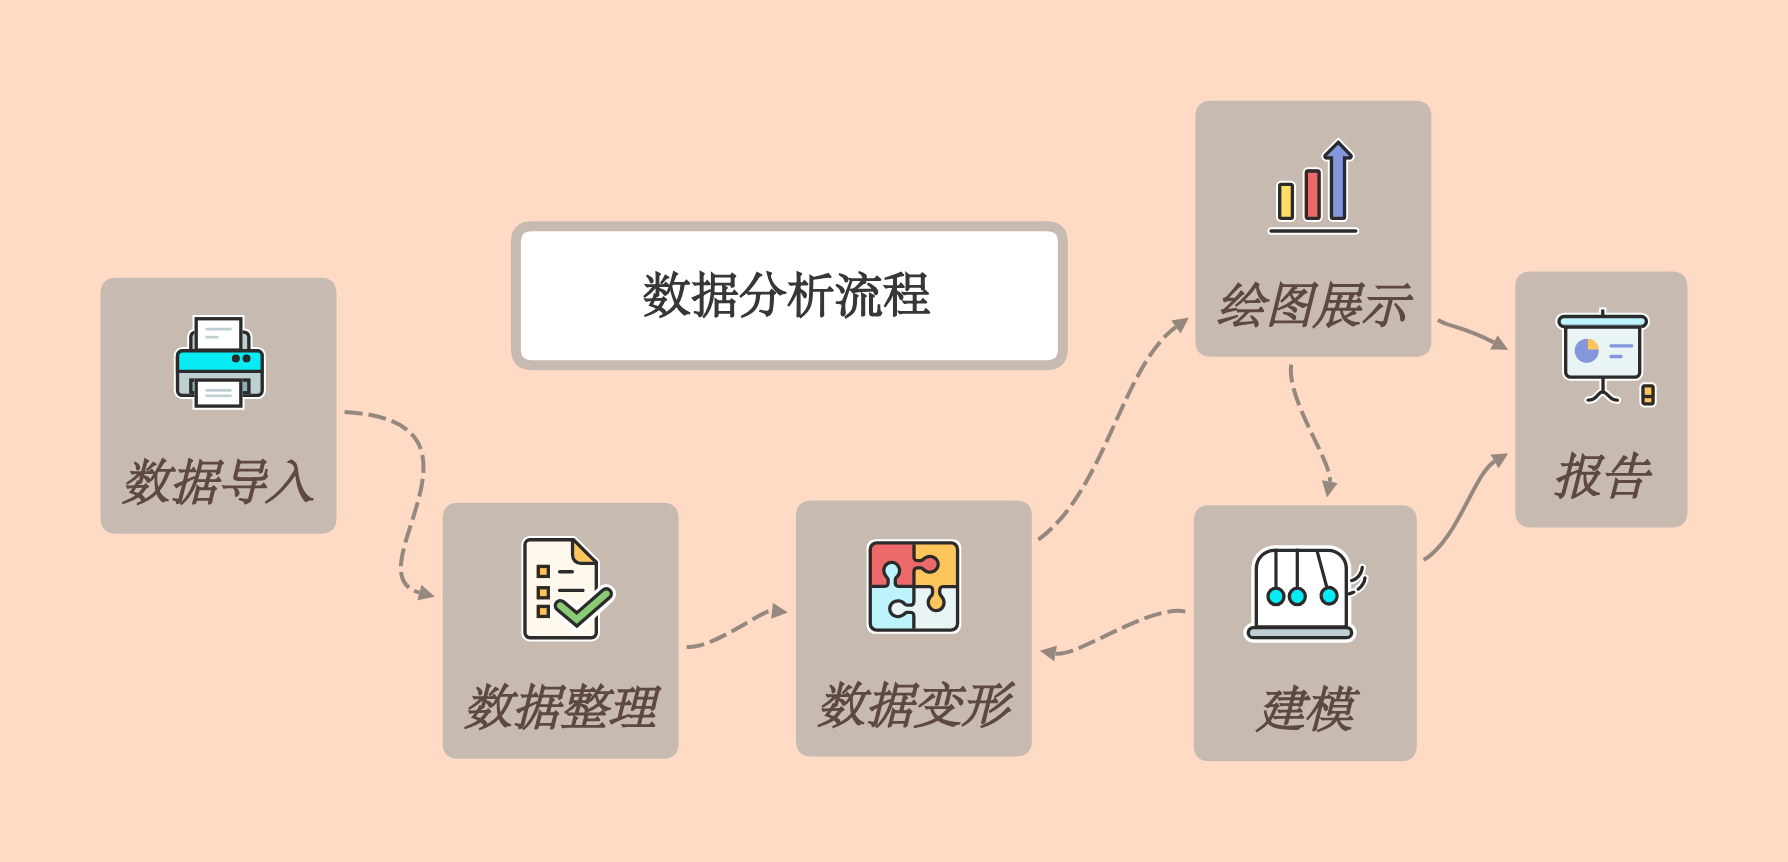
\includegraphics[width=\textwidth]{assets/数据分析流程.png}
  \caption{数据分析的基本流程}\label{fig:datawf}
\end{figure}

在这一部分你会学习到一些有用的工具:

\begin{enumerate}
\item  绘图是学习 Stata 的一个很好的开始,这是因为绘图能够最快地给使用者成就感。在数据可视化部分你讲学习到一些基本的绘图方法和一些有用的数据处理技巧。
\item  仅仅学习绘图是不够的,你还需要学习一些数据变换的方法,这样你才能根据自己的需要展示数据。
\item  最后,当你掌握了一些数据变换和绘图的方法之后,你就可以对一些实际案例进行分析了。
\end{enumerate}

接下来的三章将分别介绍数据可视化、数据整理和数据探索性分析。

\section{准备工作}

作者认为 Stata 的默认绘图主题不怎么好看,所以建议不要使用,推荐使用 plotplain 主题,安装方法如下:

\begin{lstlisting}
* 安装主题包
net install gr0070, from("http://www.stata-journal.com/software/sj17-3") replace
* 设置 plotplain 会默认绘图主题
set scheme plotplain, permanently
\end{lstlisting}

关于 Stata 绘图主题的选择,可以参考 \href{https://blog.stata.com/2018/10/02/scheming-your-way-to-your-favorite-graph-style/}{Scheming your way to your favorite graph style} 和 \href{https://www.czxa.top/posts/24695/}{Stata的绘图主题}。

\section{第一步}

\begin{problem}
  让我们用图表回答这么一个问题:大排量的汽车是否比小排量的汽车使用更多的燃料?你可能已经有了答案,但是图表可以让你的答案更有说服力,发动机的功率和燃油效率之间的关系是怎样的,是正相关么?是线性的么?
\end{problem}

\subsection{读入 mpg 数据}

这个数据集来源于 R 的 ggplot2 包,mpg 数据集包含了美国环保局收集的 38 种型号的汽车的数据:

\begin{lstlisting}
cd ~/Documents/我的项目/stata4ds/
sysuse mpg, clear
\end{lstlisting}

表 \ref{tab:mpg} 展示了 mpg 数据集的一部分。

\begin{table}[htbp]
\caption{\label{tab:mpg}mpg 数据概览}
\centering
\begin{tabular}{ccccccccccc}
\toprule
manufacturer & model & displ & year & cyl & trans & drv & cty & hwy & fl & class\\
\midrule
audi & a4 & 1.8 & 1999 & 4 & auto(l5) & f & 18 & 29 & p & compact\\
audi & a4 & 1.8 & 1999 & 4 & manual(m5) & f & 21 & 29 & p & compact\\
audi & a4 & 2.0 & 2008 & 4 & manual(m6) & f & 20 & 31 & p & compact\\
audi & a4 & 2.0 & 2008 & 4 & auto(av) & f & 21 & 30 & p & compact\\
audi & a4 & 2.8 & 1999 & 6 & auto(l5) & f & 16 & 26 & p & compact\\
\addlinespace
audi & a4 & 2.8 & 1999 & 6 & manual(m5) & f & 18 & 26 & p & compact\\
audi & a4 & 3.1 & 2008 & 6 & auto(av) & f & 18 & 27 & p & compact\\
audi & a4 quattro & 1.8 & 1999 & 4 & manual(m5) & 4 & 18 & 26 & p & compact\\
audi & a4 quattro & 1.8 & 1999 & 4 & auto(l5) & 4 & 16 & 25 & p & compact\\
audi & a4 quattro & 2.0 & 2008 & 4 & manual(m6) & 4 & 20 & 28 & p & compact\\
\bottomrule
\end{tabular}
\end{table}

其中:
1. dipl 变量为发动机的排量,单位为升;
2. hwy 变量是汽车在高速公路上的燃油效率,以每加仑汽油前进英里数(mpg)计算。当行驶相同距离时,具有低燃油效率的汽车消耗更多的燃料。

\subsection{创建散点图}

\texttt{scatter} 命令的基本用法是 \texttt{scatter\ y\ x},如图 \ref{fig:hwydispl}:

\begin{lstlisting}
twoway scatter hwy displ
\end{lstlisting}

\begin{figure}[htbp]
  \centering
  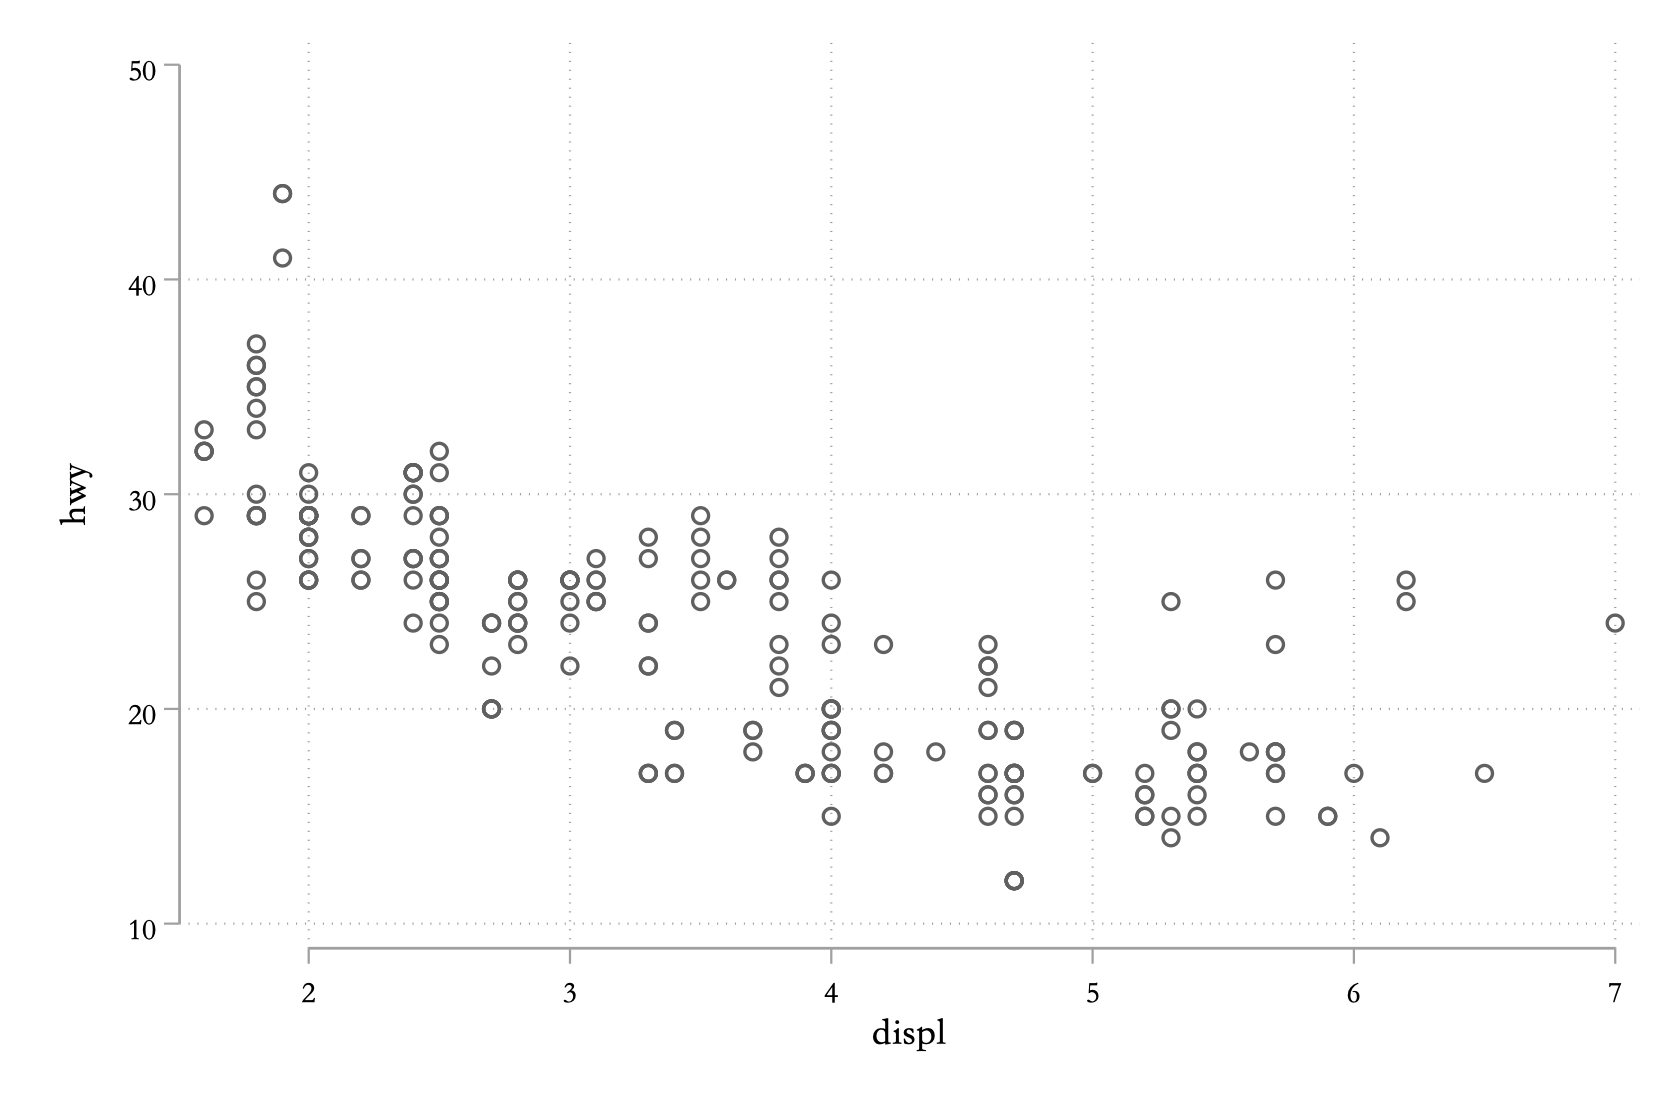
\includegraphics[width=\textwidth]{assets/hwydispl.png}
  \caption{汽车排量与燃油效率}
  \label{fig:hwydispl}
\end{figure}

图 \ref{fig:hwydispl} 显示了发动机排量和燃油效率之间的负相关关系,换句话来说,汽车的排量越高,燃油效率越低。

\subsection{练习}

\begin{exercise}
  运行 \lstinline{sc hwy displ},你看到了什么?
\end{exercise}

\begin{solution}
  scatter 命令可以被简写为 sc, 当要绘制的图层只有一个时,twoway(可以简写为 tw)是可以省略的。
\end{solution}

\begin{exercise}
  \texttt{mpg} 数据有多少行?多少列?
\end{exercise}

\begin{solution}
  \begin{lstlisting}
  sum
  *>     Variable |        Obs        Mean    Std. Dev.       Min        Max
  *> -------------+---------------------------------------------------------
  *> manufacturer |          0
  *>        model |          0
  *>        displ |        234    3.471795    1.291959        1.6          7
  *>         year |        234      2003.5    4.509646       1999       2008
  *>          cyl |        234    5.888889    1.611534          4          8
  *> -------------+---------------------------------------------------------
  *>        trans |          0
  *>          drv |          0
  *>          cty |        234    16.85897    4.255946          9         35
  *>          hwy |        234    23.44017    5.954643         12         44
  *>           fl |          0
  *> -------------+---------------------------------------------------------
  *>        class |          0
  \end{lstlisting}

  可以看出 mpg 数据集有 11 个变量和 234 个观测值。除此之外,\texttt{count} 命令可以用于观测值计数:

  \begin{lstlisting}
  count
  *> 234
  \end{lstlisting}

  \texttt{ds} 变量可以列示出符合条件的变量,默认列示出所有变量:

  \begin{lstlisting}
  ds
  *> manufacturer  displ         cyl           drv           hwy           class
  *> model         year          trans         cty           fl

  * 查看上面命令运行产生的返回值
  return list
  *> macros:
  *>     r(varlist) : "manufacturer model displ year cyl trans drv cty hwy fl c.."

  * 返回值可以被后续的程序使用
  di "`r(varlist)'"
  *> manufacturer model displ year cyl trans drv cty hwy fl class

  * `r(varlist)' 是一个字符串,wordcount() 函数可以用于计算字符串的中包含的单词个数
  di wordcount("`r(varlist)'")
  *> 11
  \end{lstlisting}

  关于 \texttt{ds} 命令的使用可以参考其帮助文档(help ds) 或者我的博客文章: \href{https://www.czxa.top/posts/44612/\#ds\%E5\%91\%BD\%E4\%BB\%A4\%EF\%BC\%9A\%E5\%88\%97\%E5\%87\%BA\%E7\%AC\%A6\%E5\%90\%88\%E6\%9D\%A1\%E4\%BB\%B6\%E7\%9A\%84\%E5\%8F\%98\%E9\%87\%8F\%E5\%90\%8D\%E7\%A7\%B0}{Stata中的变量名与标签\#ds命令:列出符合条件的变量名称}

  最后你还可以使用 c 类返回值 c(N) 和 c(k) 查看当前数据集的观测值个数和变量的个数。关于 c 类返回值的更多内容将会在下一章介绍。

  \begin{lstlisting}
  di c(N)
  *> 74

  di c(k)
  *> 11
  \end{lstlisting}
\end{solution}

\begin{exercise}
  如何查看变量 drv 的描述性统计?
\end{exercise}

\begin{solution}
  \begin{lstlisting}
  sum drv
  *>     Variable |        Obs        Mean    Std. Dev.       Min        Max
  *> -------------+---------------------------------------------------------
  *>          drv |          0
  \end{lstlisting}

  这是因为 drv 是一个字符串变量,我们无法使用 summarize 变量对其进行描述性统计。不过 codeook 命令也能对变量进行描述:

  \begin{lstlisting}
  codebook drv
  *> ---------------------------------------------------------------------
  *> drv                                                       (unlabeled)
  *> ---------------------------------------------------------------------
  *>
  *>                   type:  string (str1)
  *>
  *>          unique values:  3                        missing "":  0/234
  *>
  *>             tabulation:  Freq.  Value
  *>                            103  "4"
  *>                            106  "f"
  *>                             25  "r"
  \end{lstlisting}

  从上面的结果可以看出,drv 变量是字符串变量、只有3种值,没有缺失值。\texttt{unlabeled} 表示该变量没有数值标签(help label)。
\end{solution}

\begin{exercise}
  绘制 hwy 对 cyl 的散点图。
\end{exercise}

\begin{solution}
  \begin{lstlisting}
  sc hwy cyl
  \end{lstlisting}

  \begin{figure}[htbp]
    \centering
    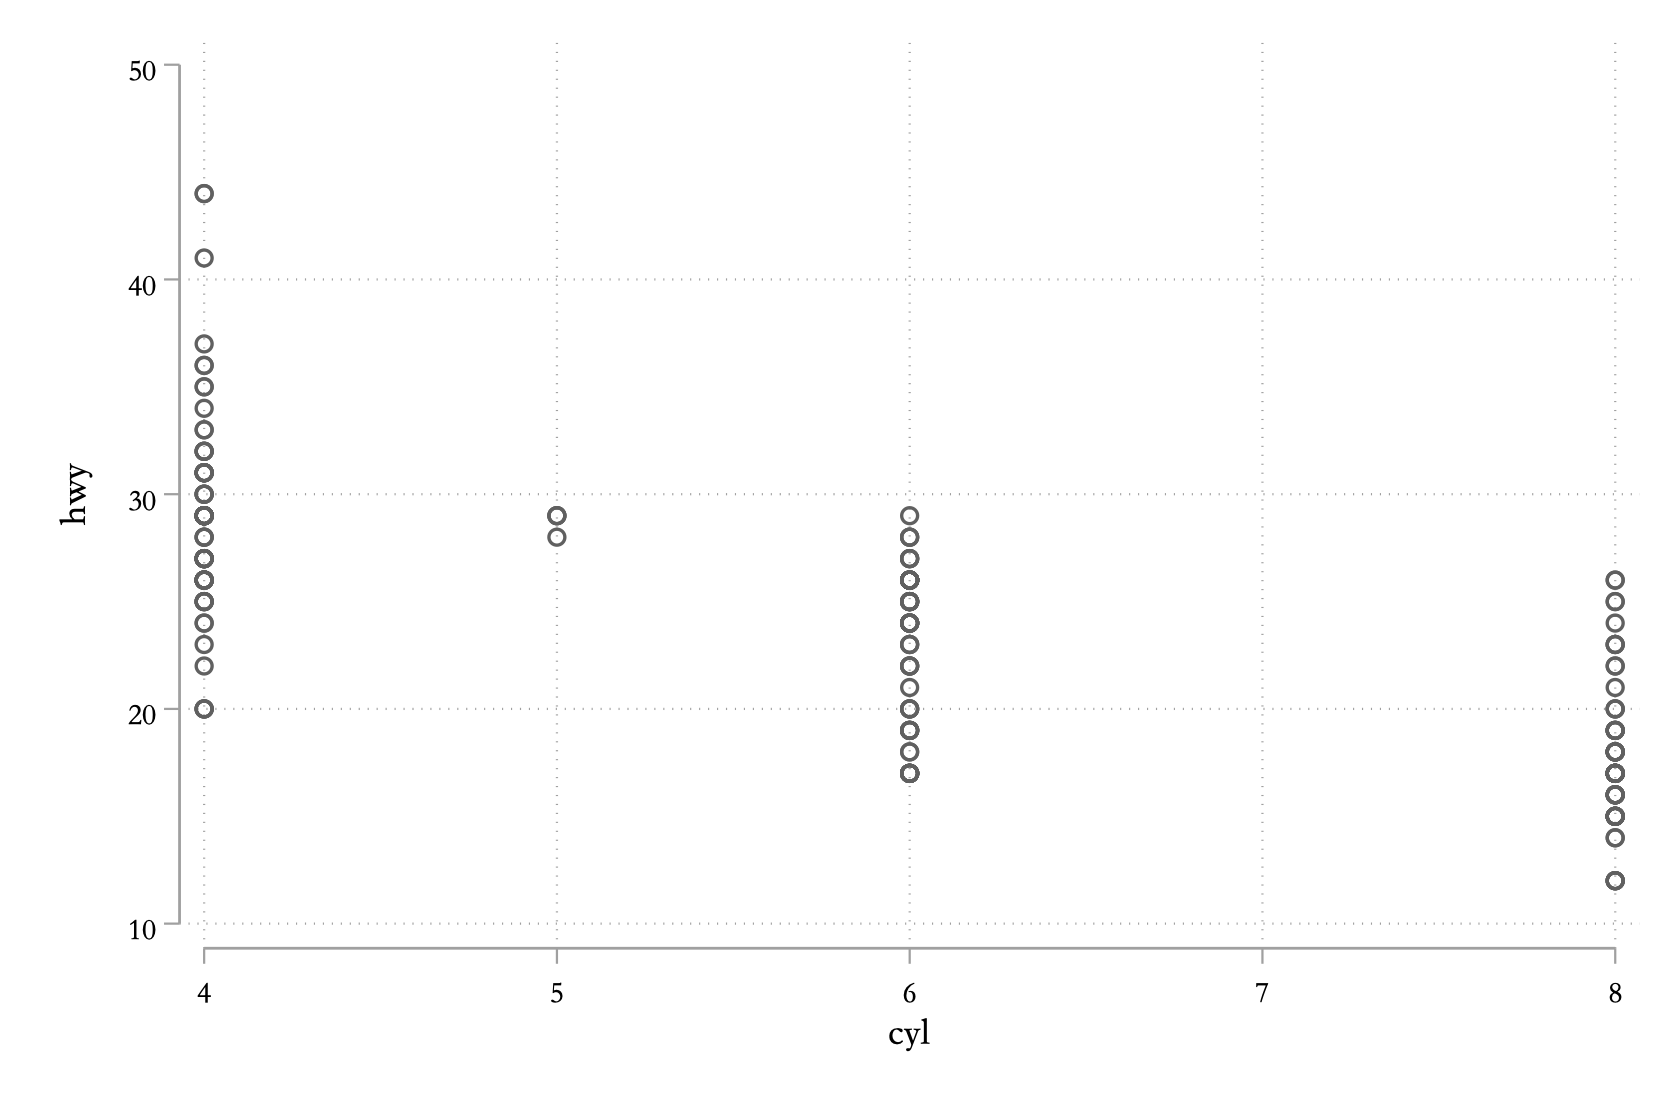
\includegraphics[width=\textwidth]{assets/hwycyl.png}
    \caption{hwy 和 cyl 的关系}
    \label{fig:hwycyl}
  \end{figure}
\end{solution}

\begin{exercise}
  如果你绘制 class 变量和 drv 变量的散点图会发生什么?为什么?
\end{exercise}

\begin{solution}
  \begin{lstlisting}
  sc class drv
  *> string variables not allowed in varlist;
  *> class is a string variable
  *> r(109);
  \end{lstlisting}

  这是因为 Stata 绘图中,字符串变量无法直接被转换成数值变量,所以不能直接用于绘图,所以我们需要首先把字符串变量转换成数值变量再进行绘图,如图 \ref{fig:classnumdrvnum}:

  \begin{lstlisting}
  encode class, gen(classnum) label(class)
  encode drv, gen(drvnum) label(drv)
  sc classnum drvnum
  \end{lstlisting}

  \begin{figure}[htbp]
    \centering
    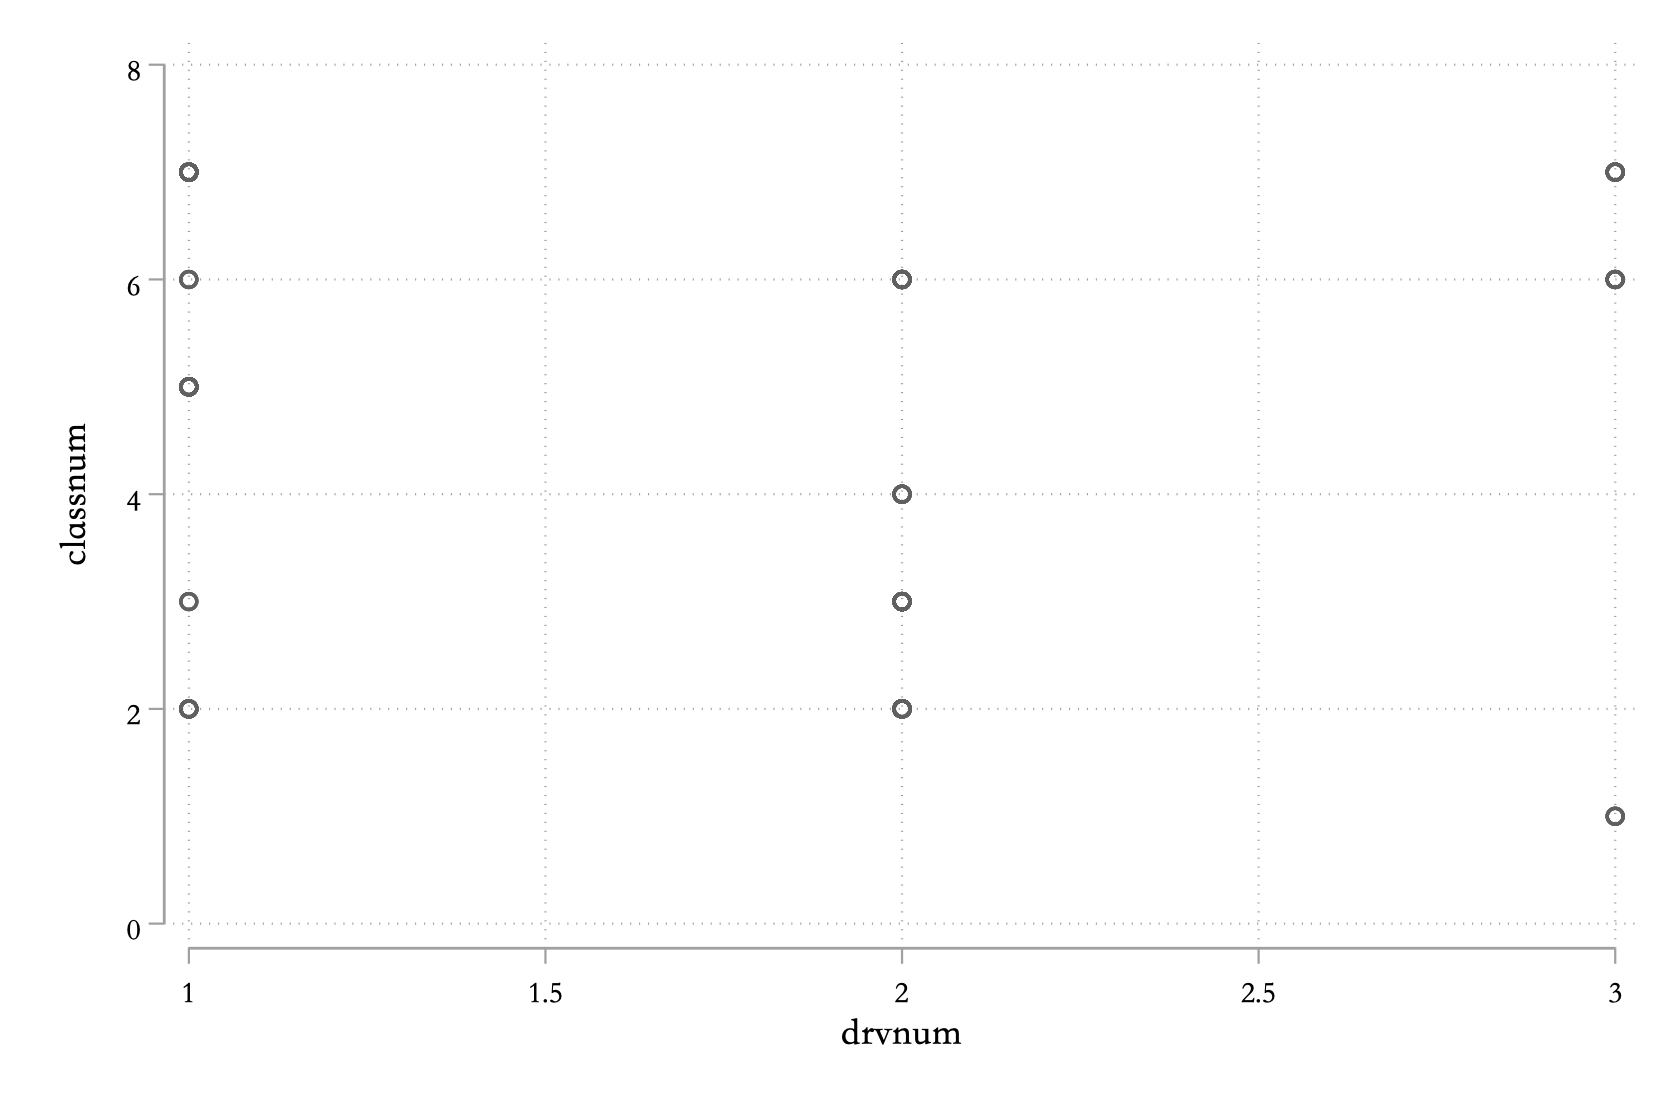
\includegraphics[width=\textwidth]{assets/classnumdrvnum.png}
    \caption{class 和 drv 的关系}
    \label{fig:classnumdrvnum}
  \end{figure}

  我们还可以使用变量的赋值标签作为轴标签,如图 \ref{fig:classnumdrvnum2}:

  \begin{lstlisting}
  sc classnum drvnum, xlab(1 2 3, val) ylab(, val)
  \end{lstlisting}

  \begin{figure}[htbp]
    \centering
    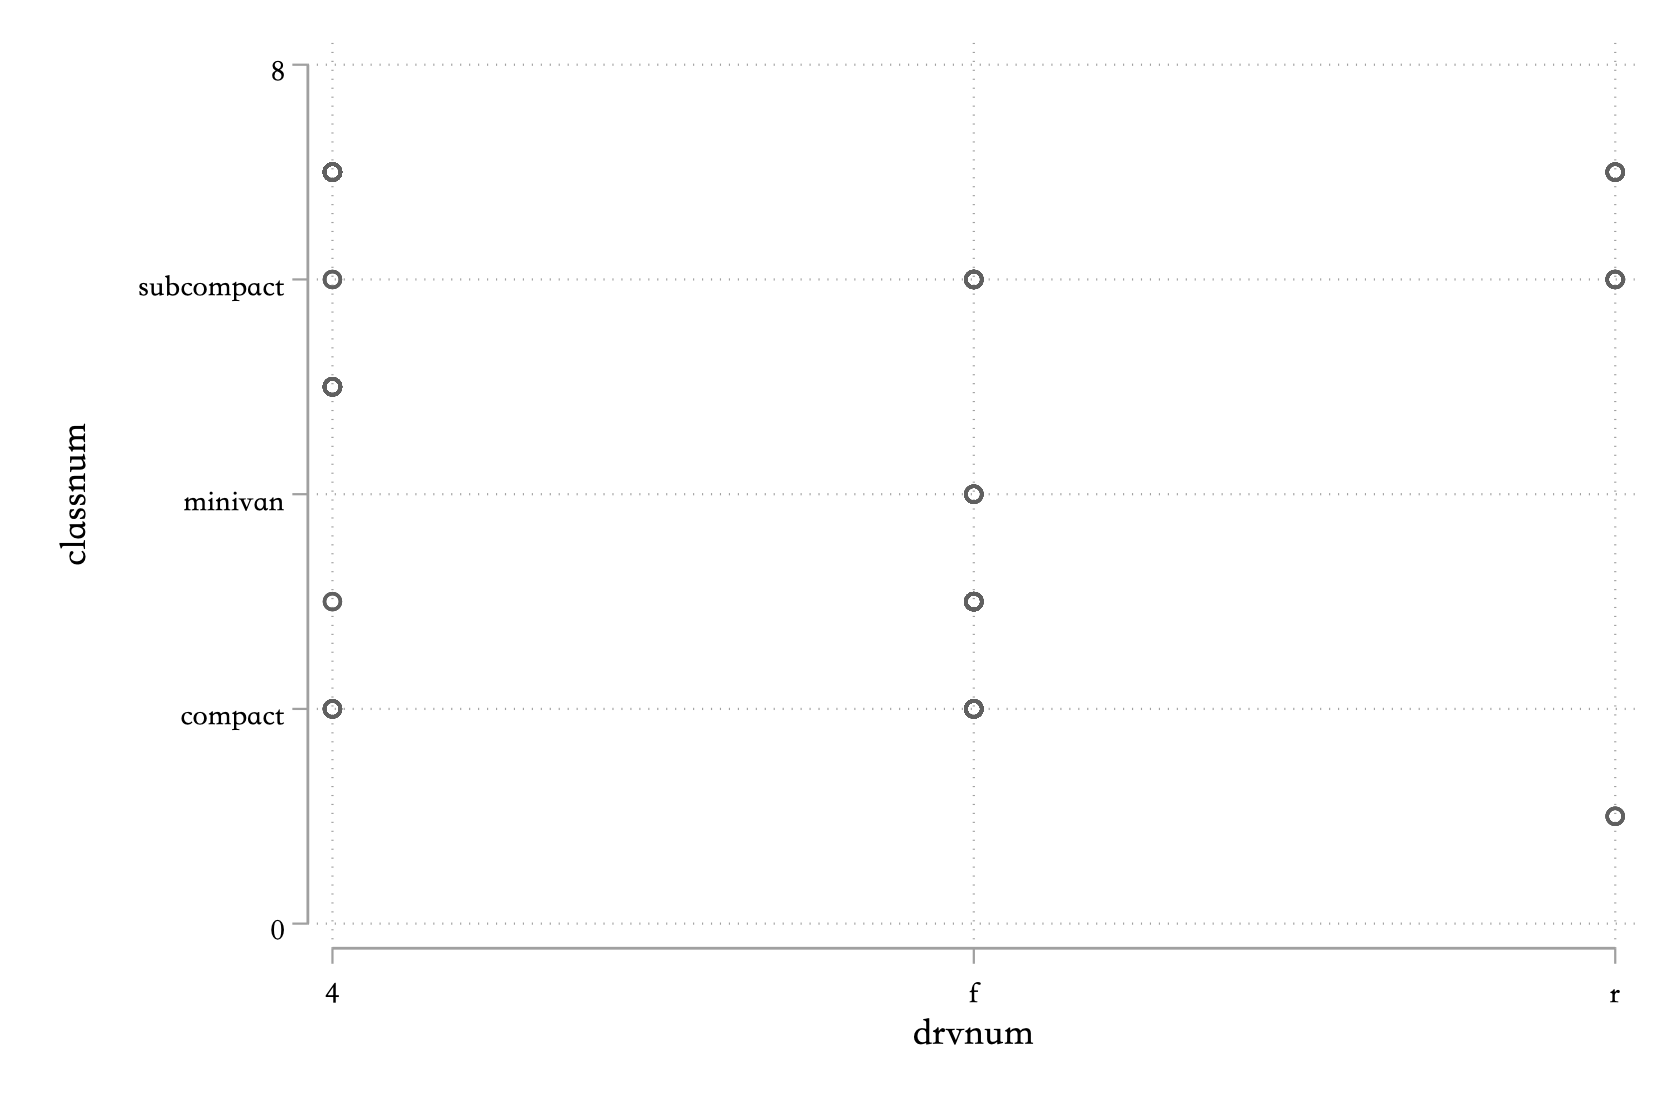
\includegraphics[width=\textwidth]{assets/classnumdrvnum2.png}
    \caption{class 和 drv 的关系}
    \label{fig:classnumdrvnum2}
  \end{figure}

  这里使用了两个选项,xlab() 选项用于控制 x 轴的标签,\texttt{1 2 3} 表示 x 轴上只显示 \texttt{1 2 3} 三个标签,对应的赋值标签正好是 \texttt{4 f r}。val 是 xlab() 选项的选项,所以它的前面用逗号隔开,表示使用赋值标签作为轴标签。
\end{solution}

\section{散点图进阶}
\begin{quote}
``The greatest value of a picture is when it forces us to notice what we never expected to see.'' --- John Tukey
\end{quote}

在图 \ref{fig:hwydispl2} 中,用红色突出的点似乎超过了线性趋势,这些车的里程数高于我们的预期,这是为什么?

\begin{lstlisting}
tw ///
sc hwy displ if displ < 5 | hwy < 22 || ///
sc hwy displ if displ > 5 & hwy > 22, mc(red) ||, ///
leg(off)
\end{lstlisting}

\begin{figure}[htbp]
  \centering
  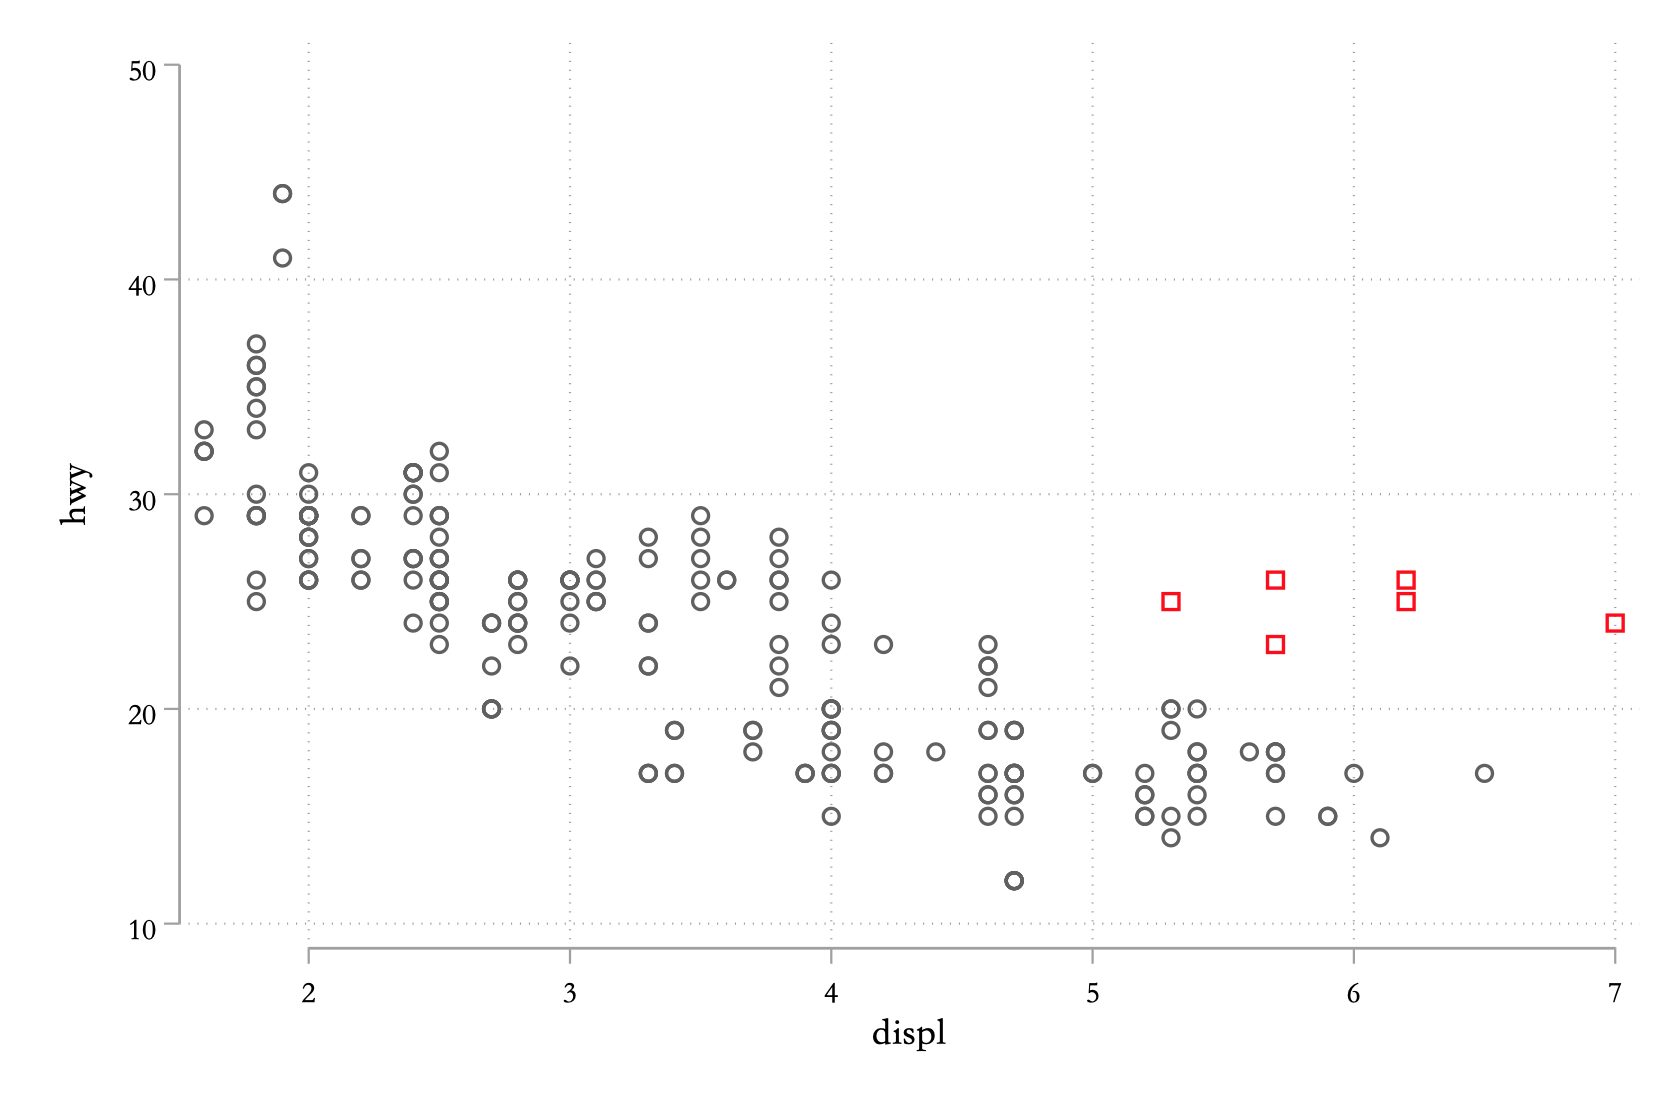
\includegraphics[width=\textwidth]{assets/hwydispl2.png}
  \caption{排量与燃油效率关系中的一些异常值}
  \label{fig:hwydispl2}
\end{figure}

这些异常值出现的一个可能的原因就是这些车中有混合动力车,检验这一猜想的办法就是查看每个 class 的 hwy,如图 \ref{fig:hwydispl3}:

\begin{lstlisting}
* 查看 class 有哪些值
levelsof class
* 可以使用 local() 选项将这些值存储为一个 local 变量
levelsof class, local(class)
* 我们可以针对 class 的每一个值绘制一个图层:
tw ///
sc hwy displ if class == "2seater" || ///
sc hwy displ if class == "compact" || ///
sc hwy displ if class == "midsize" || ///
sc hwy displ if class == "minivan" || ///
sc hwy displ if class == "pickup" || ///
sc hwy displ if class == "subcompact" || ///
sc hwy displ if class == "suv" ||, ///
leg(order(1 "2seater" ///
          2 "compact" ///
          3 "midsize" ///
          4 "minivan" ///
          5 "pickup" ///
          6 "subcompact" ///
          7 "suv") title(class))
\end{lstlisting}

\begin{figure}[htbp]
  \centering
  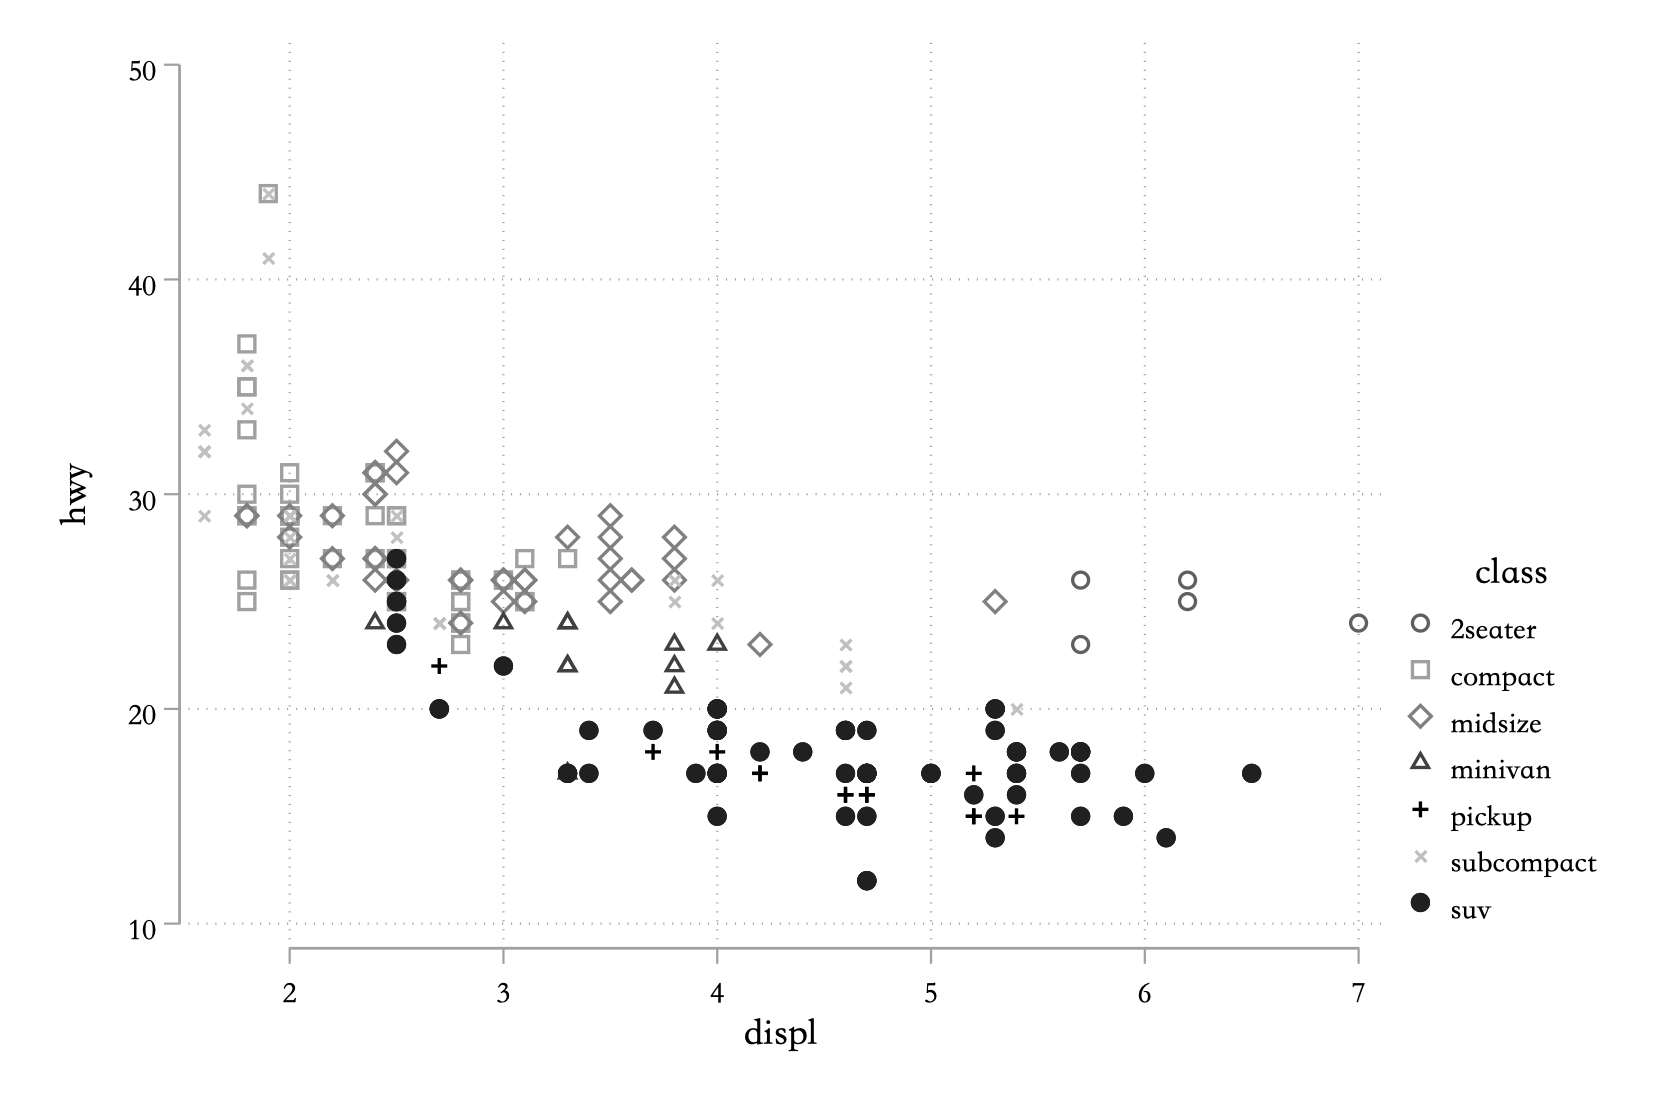
\includegraphics[width=\textwidth]{assets/hwydispl3.png}
  \caption{不同类型汽车排量与燃油效率的关系}
  \label{fig:hwydispl3}
\end{figure}

这里使用不同的散点样式表示不同图层,当然我们也可以使用不同的颜色表示,\lstinline{colorscheme} 命令是个非常好用的调色选色命令,其调色板来源于: \href{http://colorbrewer2.org/}{ColorBrewer: Color Advice for Maps},安装方式如下:

\begin{lstlisting}
net install colorscheme.pkg, from("https://github.com/matthieugomez/stata-colorscheme/raw/master/")
\end{lstlisting}

关于这个命令的使用,你可以参考其帮助文档(help colorscheme)或者我的博客文章: \href{https://www.czxa.top/posts/16049/}{colorscheme——调色选色命令}。

我最喜欢的是 \texttt{Paired} 配色方案,如图 \ref{fig:Paired}:

\begin{lstlisting}
colorscheme 12, palette(Paired) display
return list
*> macros:
*>     r(color1) : "166 206 227"
*>     r(color2) : "031 120 180"
*>     r(color3) : "178 223 138"
*>     r(color4) : "051 160 044"
*>     r(color5) : "251 154 153"
*>     r(color6) : "227 026 028"
*>     r(color7) : "253 191 111"
*>     r(color8) : "255 127 000"
*>     r(color9) : "202 178 214"
*>    r(color10) : "106 061 154"
*>    r(color11) : "255 255 153"
*>    r(color12) : "177 089 040"
*>     r(colors) : ""166 206 227" "031 120 180"  "178 223 138"  "051 160 044.."
\end{lstlisting}

\begin{figure}[htbp]
  \centering
  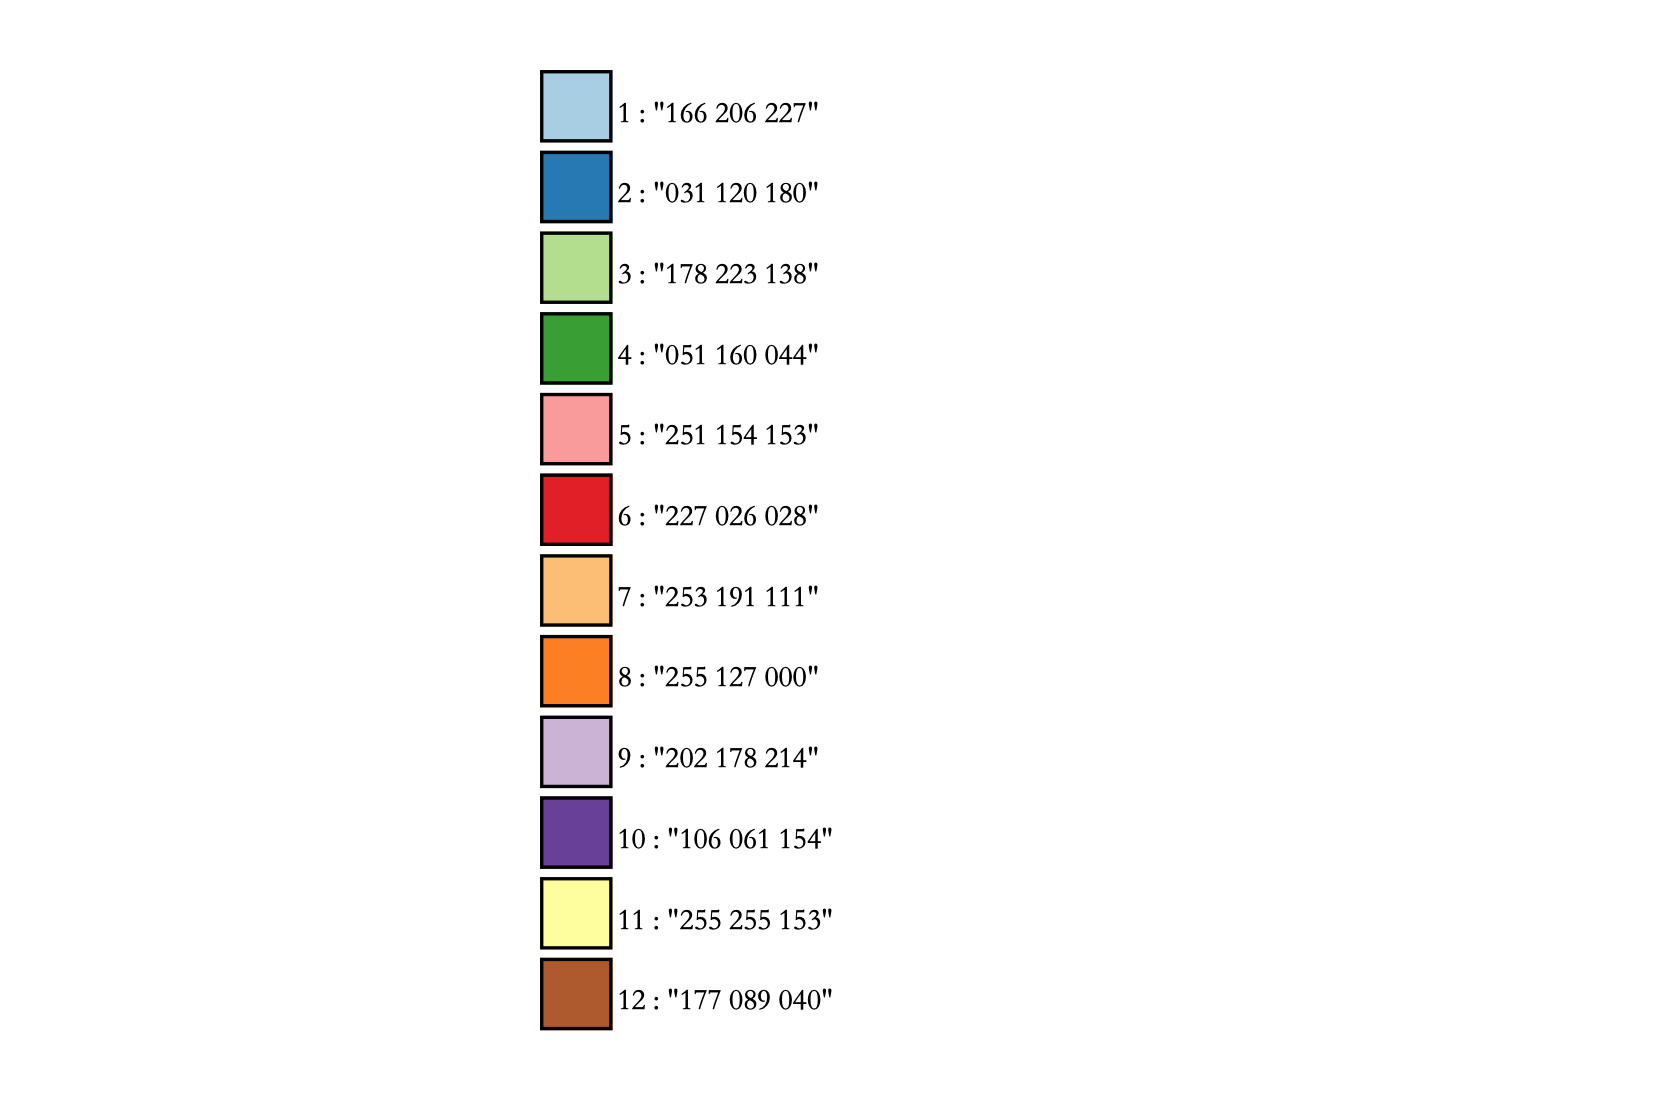
\includegraphics[width=\textwidth]{assets/Paired.png}
  \caption{Paired 配色方案}
  \label{fig:Paired}
\end{figure}

这里我们需要 7 种颜色,如图 \ref{fig:hwydispl4}:

\begin{lstlisting}
colorscheme 7, palette(Paired)
tw ///
sc hwy displ if class == "2seater", mc("`r(color1)'") ms(o) || ///
sc hwy displ if class == "compact", mc("`r(color2)'") ms(o) || ///
sc hwy displ if class == "midsize", mc("`r(color3)'") ms(o) || ///
sc hwy displ if class == "minivan", mc("`r(color4)'") ms(o) || ///
sc hwy displ if class == "pickup", mc("`r(color5)'") ms(o) || ///
sc hwy displ if class == "subcompact", mc("`r(color6)'") ms(o) || ///
sc hwy displ if class == "suv", mc("`r(color7)'") ms(o) ||, ///
leg(order(1 "2seater" ///
          2 "compact" ///
          3 "midsize" ///
          4 "minivan" ///
          5 "pickup" ///
          6 "subcompact" ///
          7 "suv") title(class))
\end{lstlisting}

\begin{figure}[htbp]
  \centering
  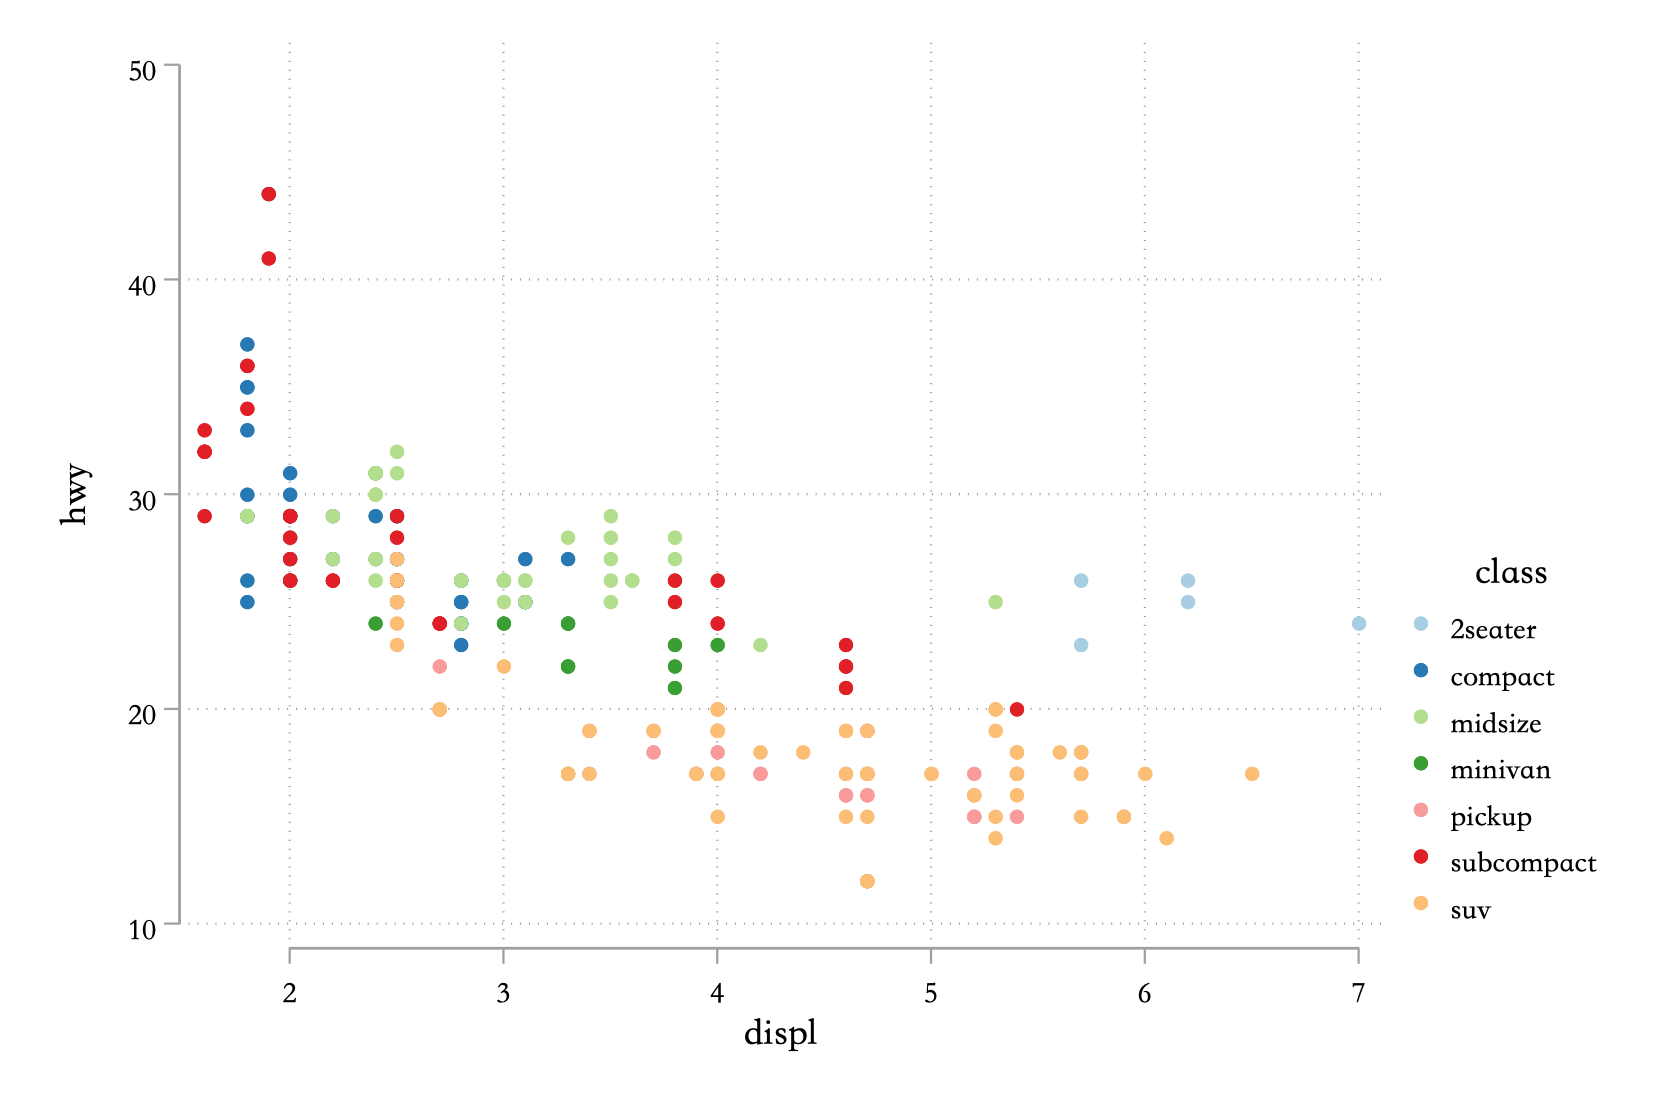
\includegraphics[width=\textwidth]{assets/hwydispl4.png}
  \caption{不同类型汽车排量与燃油效率的关系}
  \label{fig:hwydispl4}
\end{figure}

当然你也可以用散点的大小表示不同的图层,如图 \ref{fig:hwydispl5}:

\begin{lstlisting}
colorscheme 7, palette(Set2)
tw ///
sc hwy displ if class == "2seater", mc("`r(color1)'") ms(o) msize(*1) || ///
sc hwy displ if class == "compact", mc("`r(color2)'") ms(o) msize(*1.5) || ///
sc hwy displ if class == "midsize", mc("`r(color3)'") ms(o) msize(*2) || ///
sc hwy displ if class == "minivan", mc("`r(color4)'") ms(o) msize(*2.5) || ///
sc hwy displ if class == "pickup", mc("`r(color5)'") ms(o) msize(*3) || ///
sc hwy displ if class == "subcompact", mc("`r(color6)'") ms(o) msize(*3.5) || ///
sc hwy displ if class == "suv", mc("`r(color7)'") ms(o) msize(*4) ||, ///
leg(order(1 "2seater" ///
          2 "compact" ///
          3 "midsize" ///
          4 "minivan" ///
          5 "pickup" ///
          6 "subcompact" ///
          7 "suv") title(class))
\end{lstlisting}

\begin{figure}[htbp]
  \centering
  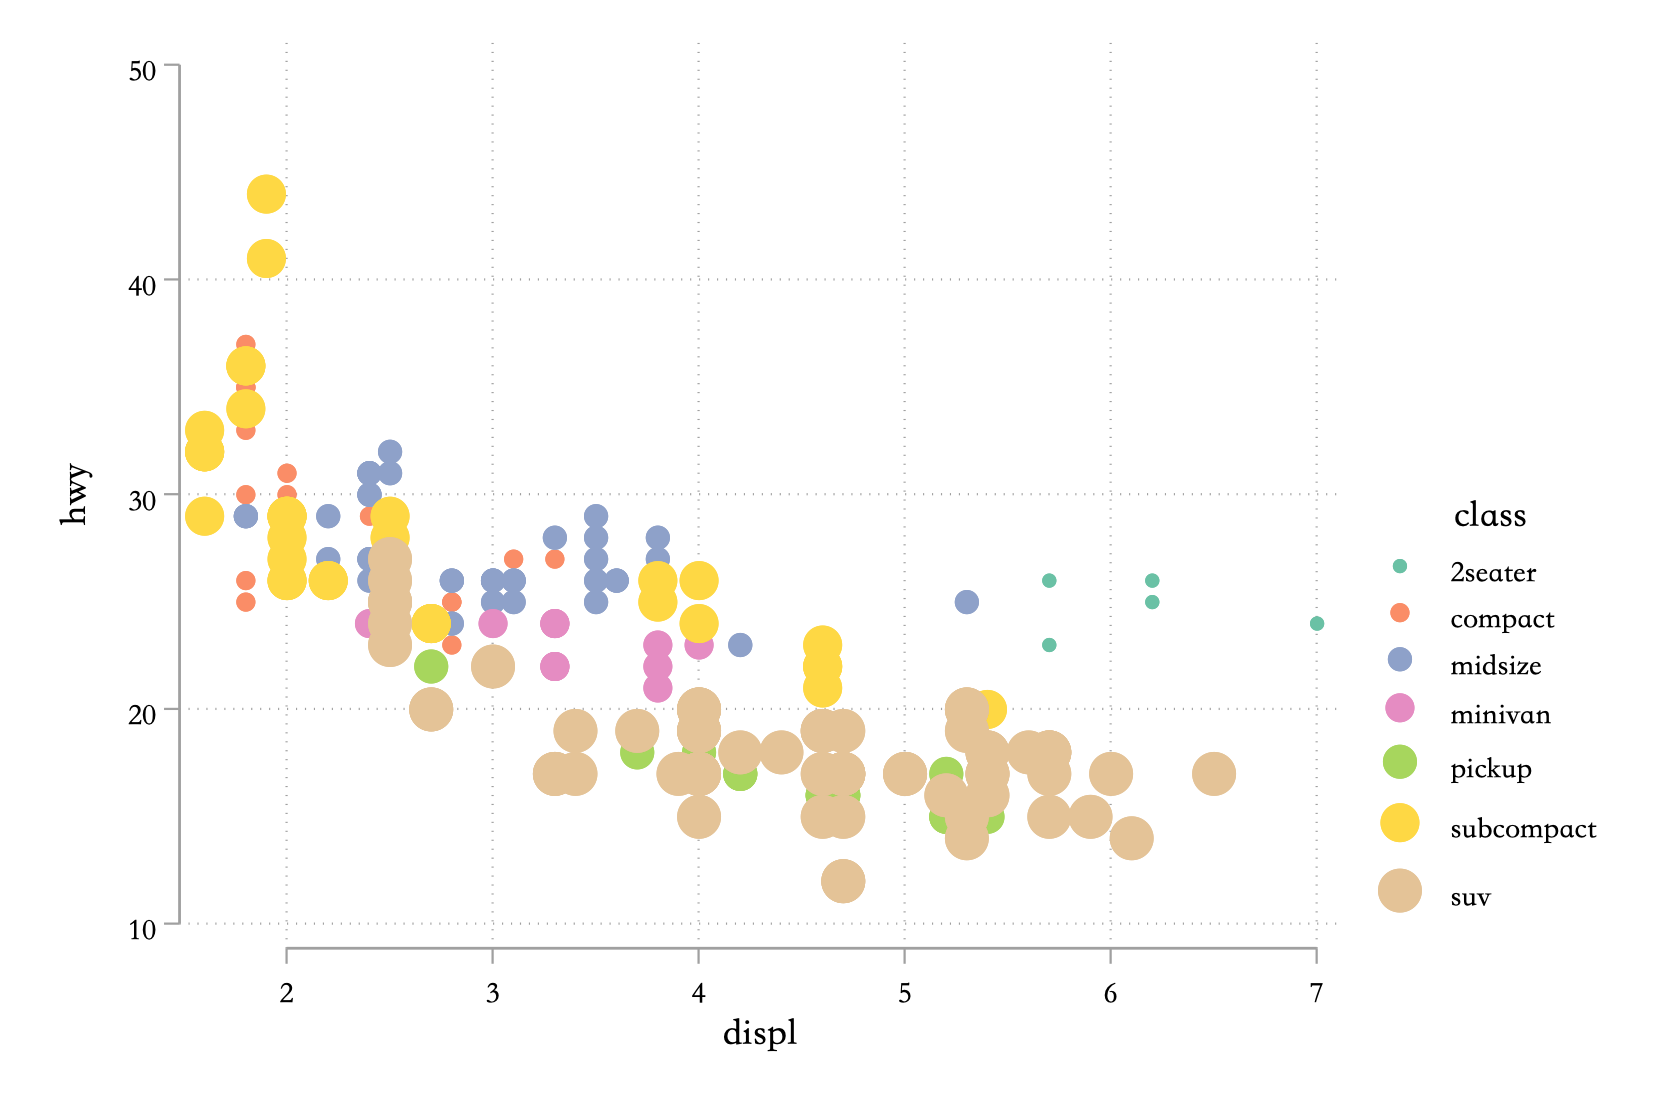
\includegraphics[width=\textwidth]{assets/hwydispl5.png}
  \caption{不同类型汽车排量与燃油效率的关系}\label{fig:hwydispl5}
\end{figure}

最后 Stata15 在绘图方面引入了一个新特性就是可以为图层设置透明度了!关于透明度的使用可以参考 Stata 官网上的相关介绍和我的博客文章: \href{https://www.czxa.top/posts/44086/}{Stata15绘图的新功能:设置图形的透明度},图 \ref{fig:hwydispl6}展示了使用透明度的效果:

\begin{lstlisting}
/* 左图 */
tw ///
sc hwy displ if class == "2seater" || ///
sc hwy displ if class == "compact" || ///
sc hwy displ if class == "midsize" || ///
sc hwy displ if class == "minivan" || ///
sc hwy displ if class == "pickup" || ///
sc hwy displ if class == "subcompact" || ///
sc hwy displ if class == "suv" ||, ///
leg(order(1 "2seater" ///
          2 "compact" ///
          3 "midsize" ///
          4 "minivan" ///
          5 "pickup" ///
          6 "subcompact" ///
          7 "suv") title(class)) name(p1) nodraw
/* 右图 */
tw ///
sc hwy displ if class == "2seater", mc(%90) ms(o) || ///
sc hwy displ if class == "compact", mc(%80) ms(o) || ///
sc hwy displ if class == "midsize", mc(%70) ms(o) || ///
sc hwy displ if class == "minivan", mc(%60) ms(o) || ///
sc hwy displ if class == "pickup", mc(%50) ms(o) || ///
sc hwy displ if class == "subcompact", mc(%40) ms(o) || ///
sc hwy displ if class == "suv", mc(%30) ms(o) ||, ///
leg(order(1 "2seater" ///
          2 "compact" ///
          3 "midsize" ///
          4 "minivan" ///
          5 "pickup" ///
          6 "subcompact" ///
          7 "suv") title(class)) name(p2) nodraw
/* 合并 */
gr combine p1 p2
\end{lstlisting}

\begin{figure}[htbp]
  \centering
  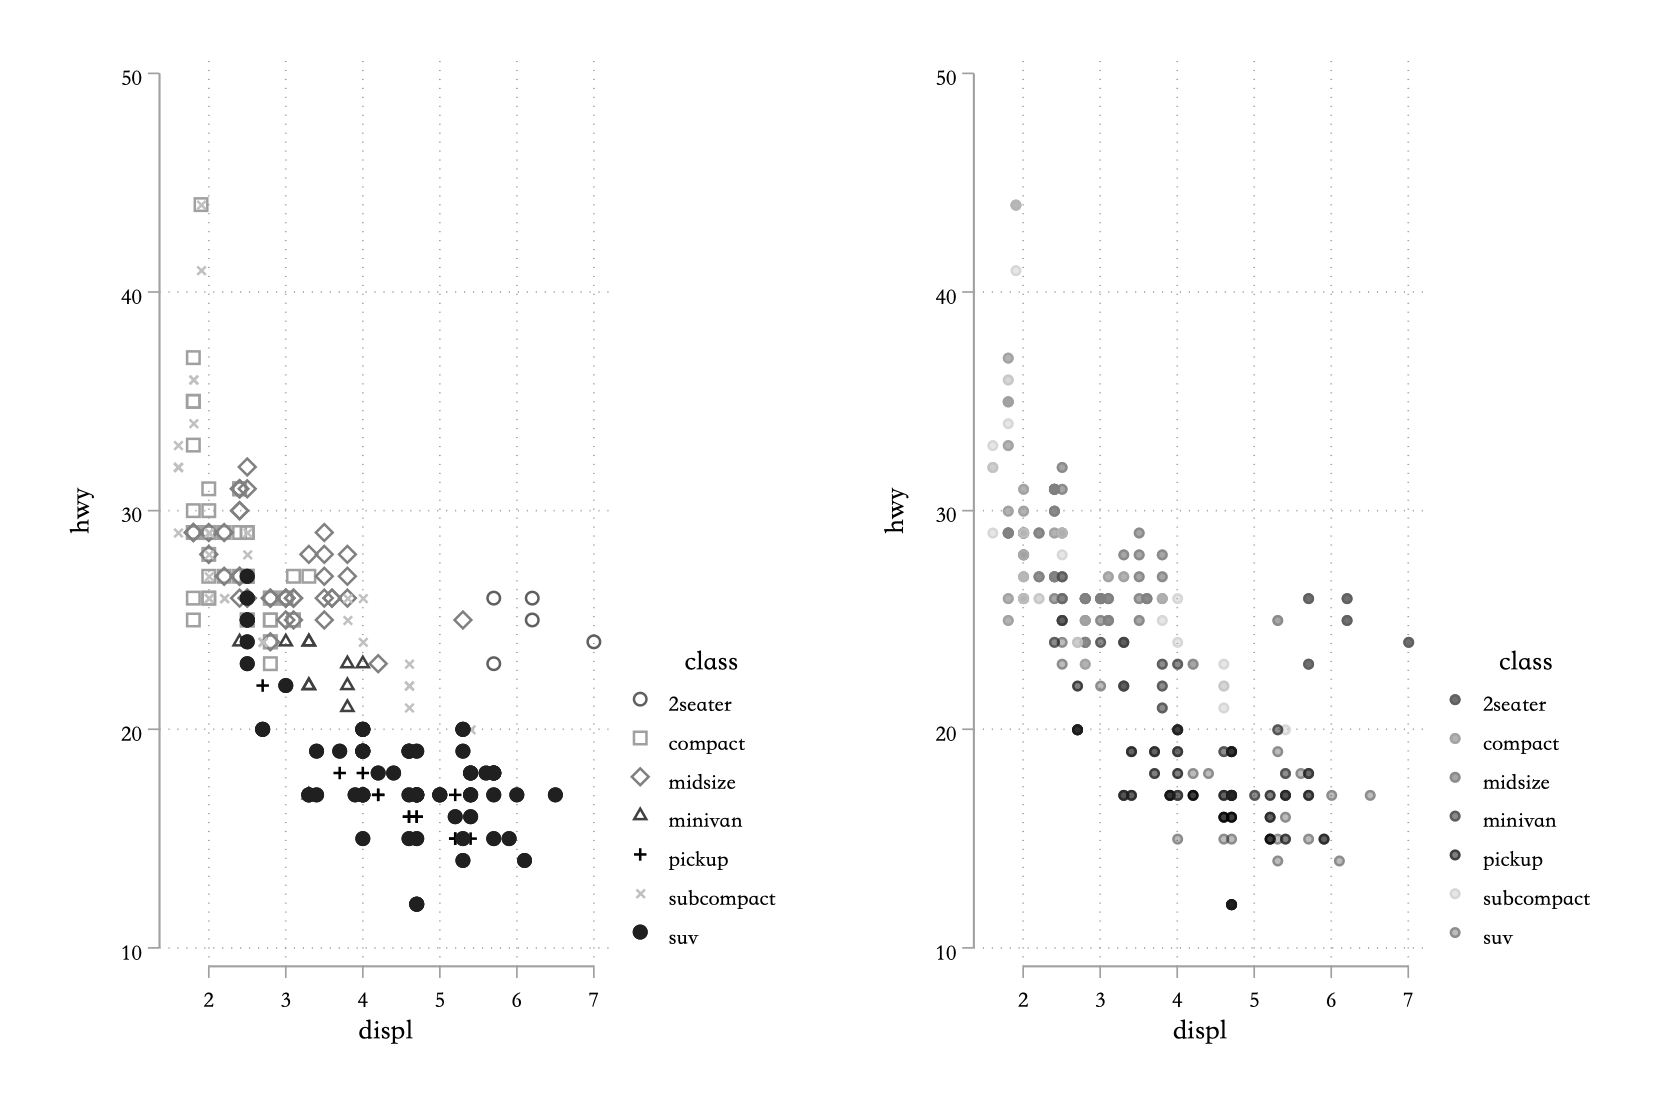
\includegraphics[width=\textwidth]{assets/hwydispl6.png}
  \caption{不同类型汽车排量与燃油效率的关系}
  \label{fig:hwydispl6}
\end{figure}

Stata 绘图中的散点样式如图 \ref{fig:symbolpalette}:

\begin{lstlisting}
palette symbolpalette
\end{lstlisting}

\begin{figure}[htbp]
  \centering
  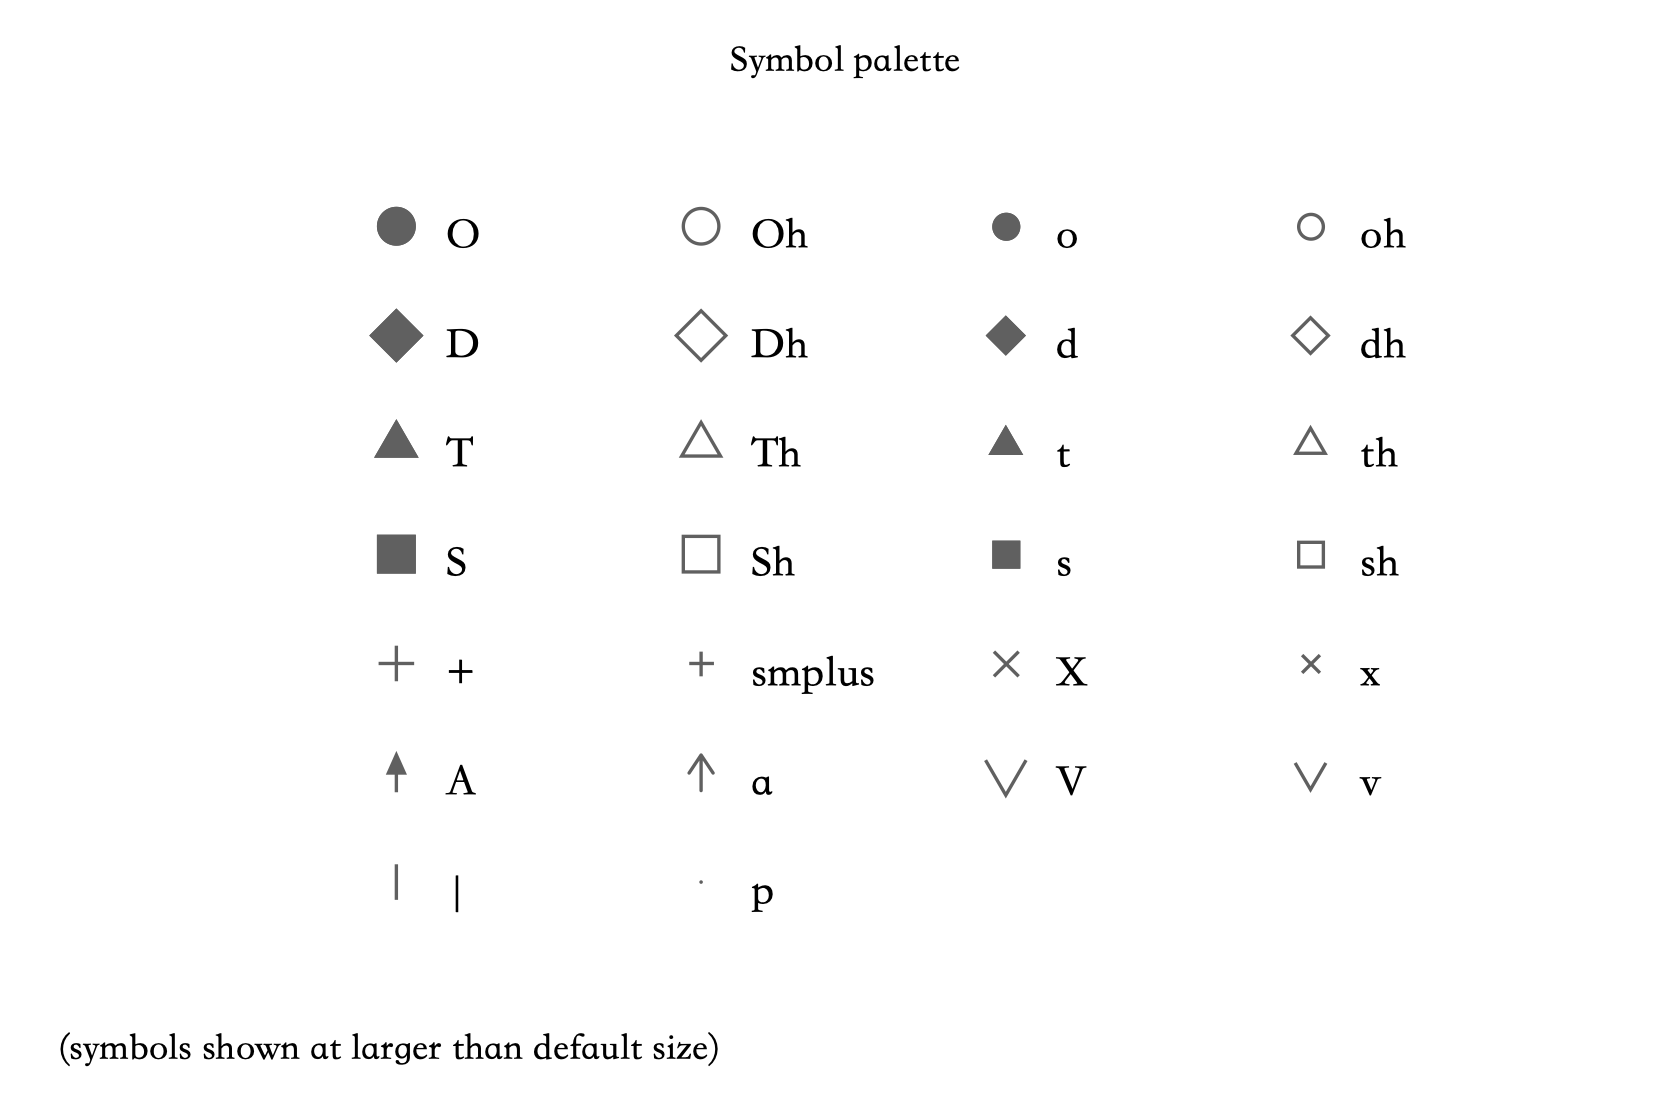
\includegraphics[width=\textwidth]{assets/symbolpalette.png}
  \caption{Stata 绘图中的散点样式}
  \label{fig:symbolpalette}
\end{figure}

\section{分面}

把多个图层叠加在一起就会产生相互重叠的问题,因此我们有时候会选择将不同的图层分开绘制,也就是分面,如图 \ref{fig:hwydisplbyclass}:

\begin{lstlisting}
sc hwy displ, by(class)
\end{lstlisting}

\begin{figure}[htbp]
  \centering
  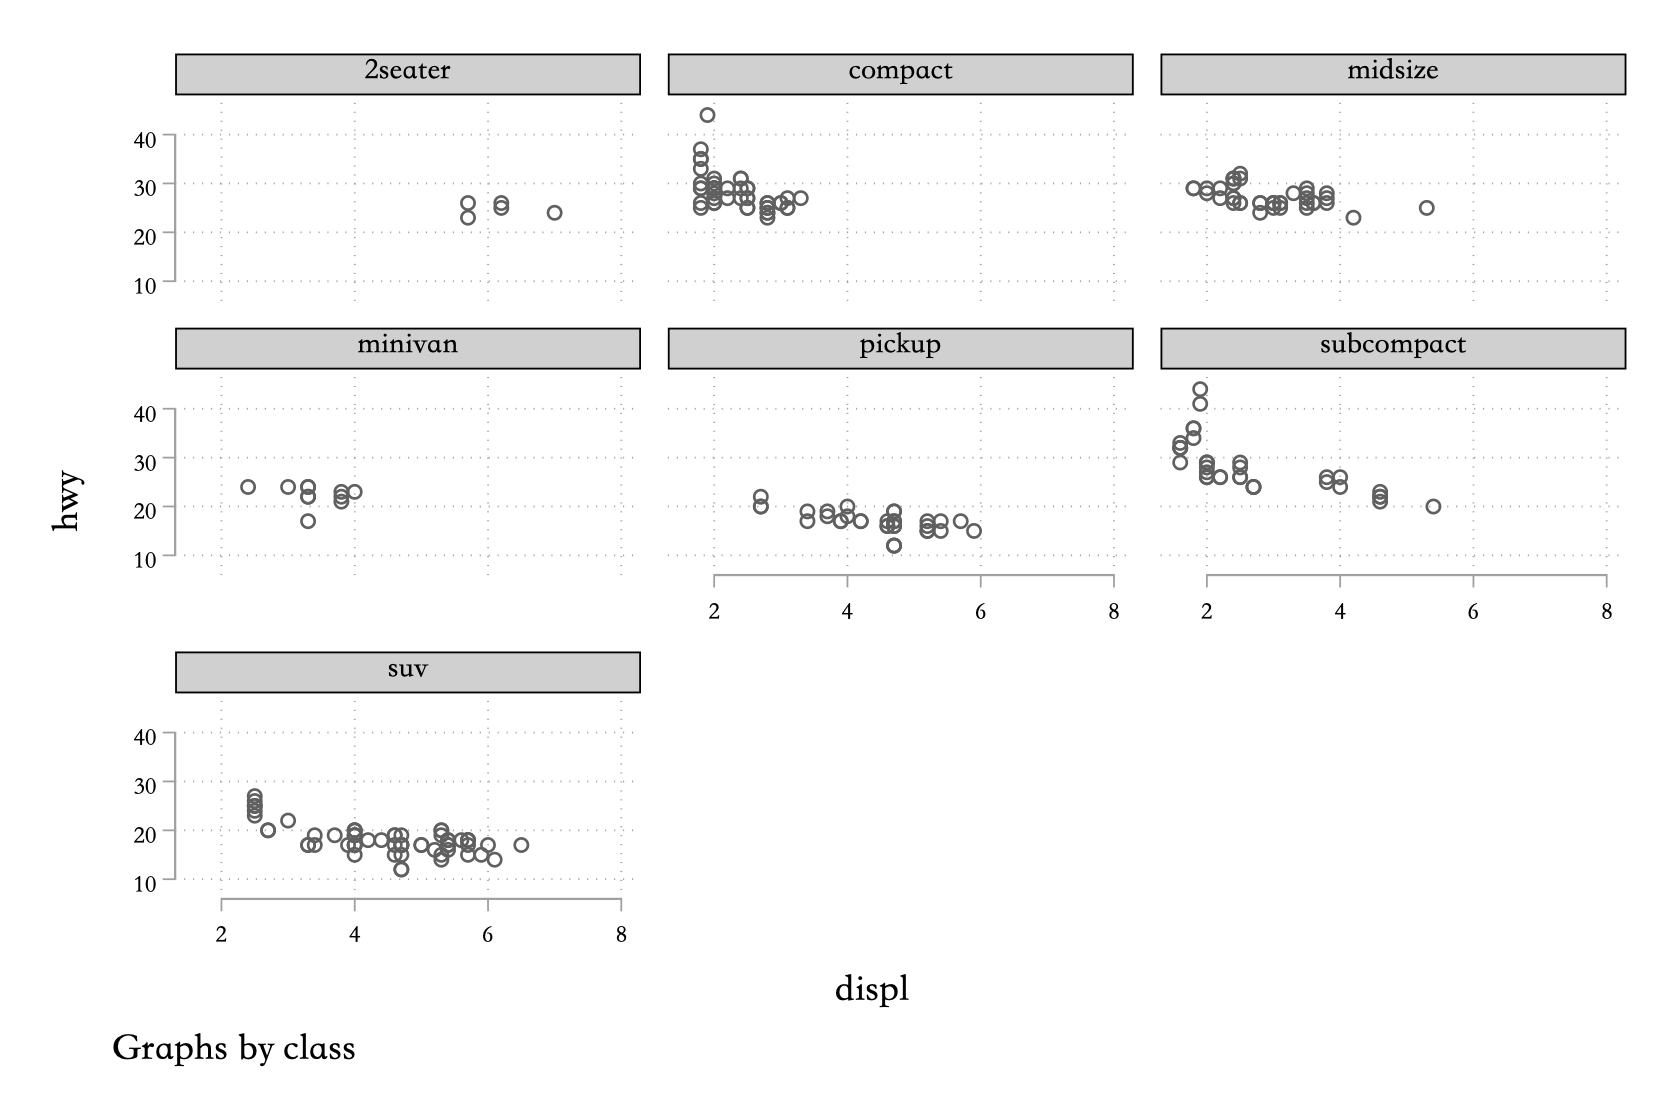
\includegraphics[width=1\textwidth]{assets/hwydisplbyclass.png}
  \caption{不同型号汽车排量与燃油效率的关系}
  \label{fig:hwydisplbyclass}
\end{figure}

我们也可以使用两个变量的组合进行分面,如图 \ref{fig:hwydisplbyfrvcyl}:

\begin{lstlisting}
sc hwy displ, by(drv cyl)
\end{lstlisting}

\begin{figure}[htbp]
  \centering
  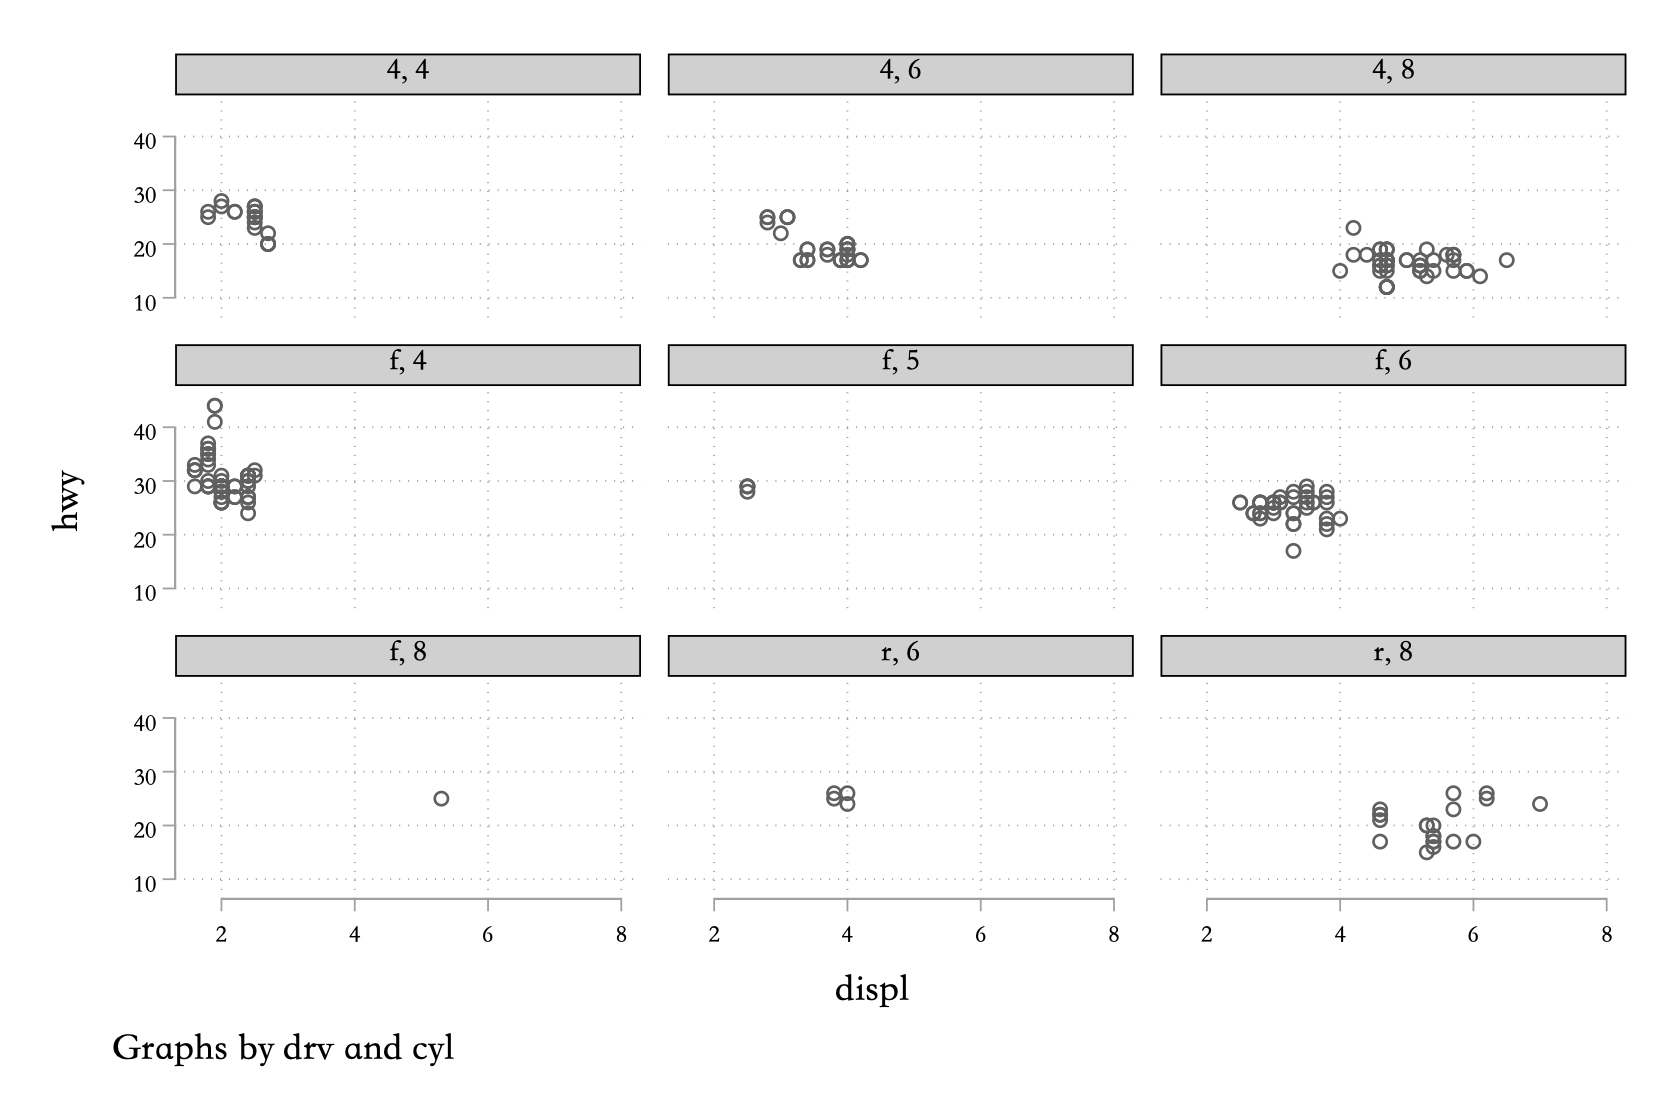
\includegraphics[width=1\textwidth]{assets/hwydisplbyfrvcyl.png}
  \caption{不同drv和cyl的汽车排量与燃油效率的关系}
  \label{fig:hwydisplbyfrvcyl}
\end{figure}

我们还可以自定义分面图的排列,例如全部排列在一行,如图 \ref{fig:hwydisplbyclass2}:

\begin{lstlisting}
sc hwy displ, by(class, row(1))
\end{lstlisting}

\begin{figure}[htbp]
  \centering
  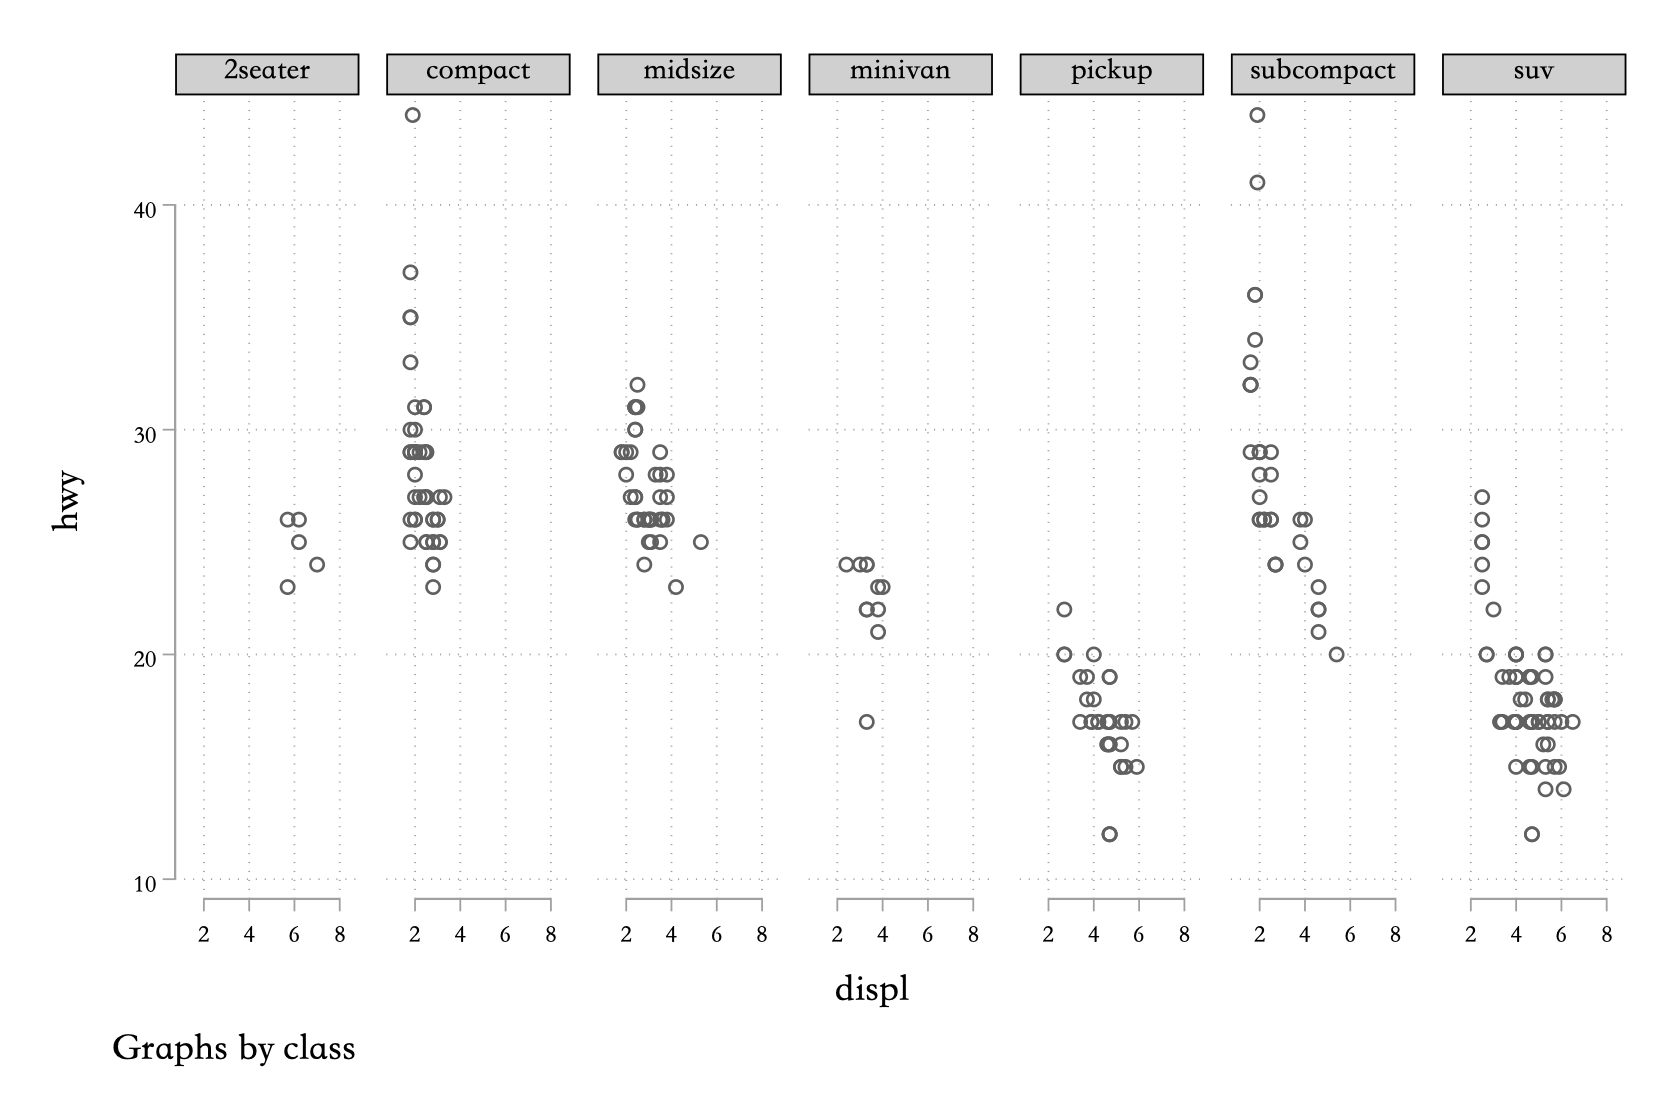
\includegraphics[width=1\textwidth]{assets/hwydisplbyclass2.png}
  \caption{不同型号汽车排量与燃油效率的关系}\label{fig:hwydisplbyclass2}
\end{figure}

经常有小伙伴在绘制分面图的时候想把左下角的 \texttt{Graphs\ by\ xx} 去掉,这个可以通过 \texttt{by()} 的子选项去除:

\begin{lstlisting}
sc hwy displ, by(class, note(""))
\end{lstlisting}

\begin{figure}[htbp]
  \centering
  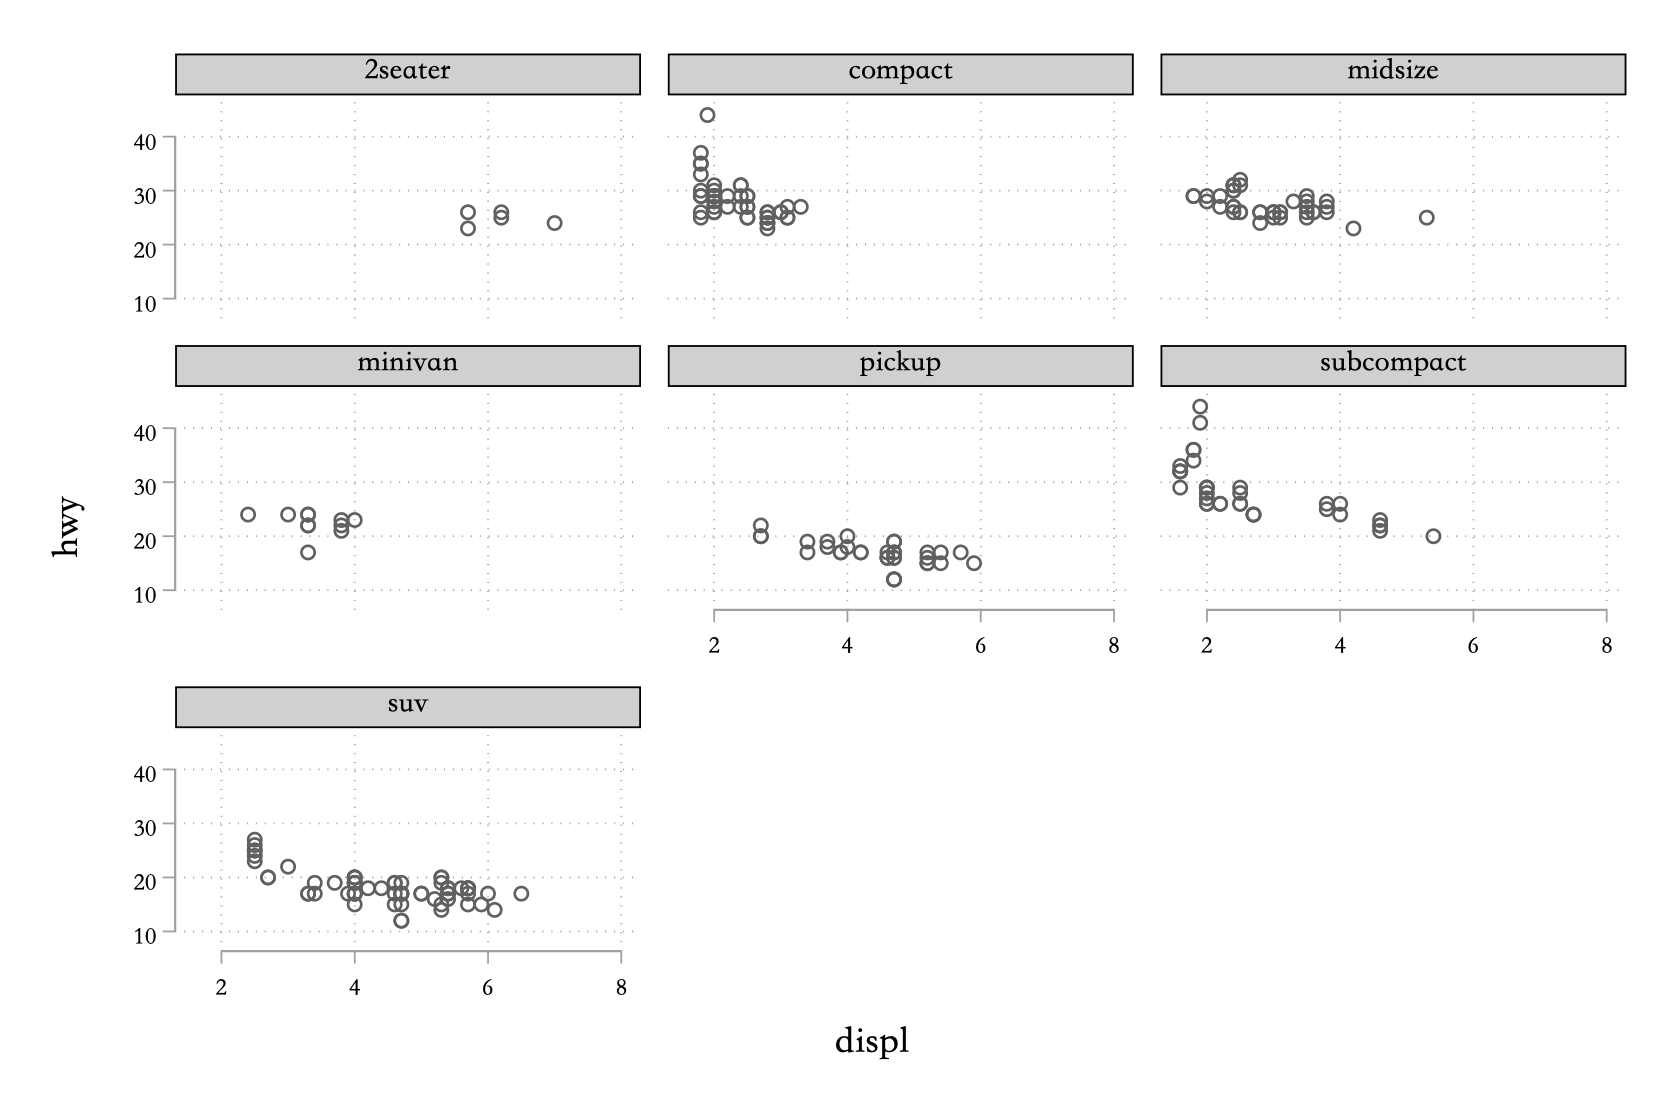
\includegraphics[width=1\textwidth]{assets/hwydisplbyclass3.png}
  \caption{不同型号汽车排量与燃油效率的关系}
  \label{fig:hwydisplbyclass3}
\end{figure}

\section{几何对象}

\begin{problem}
  观察图 \ref{fig:lpolychwydisp} 中的两个图层,什么相似的地方?

  \begin{lstlisting}
  tw ///
  sc hwy displ || ///
  lpolyci hwy disp
  \end{lstlisting}

  \begin{figure}[htbp]
    \centering
    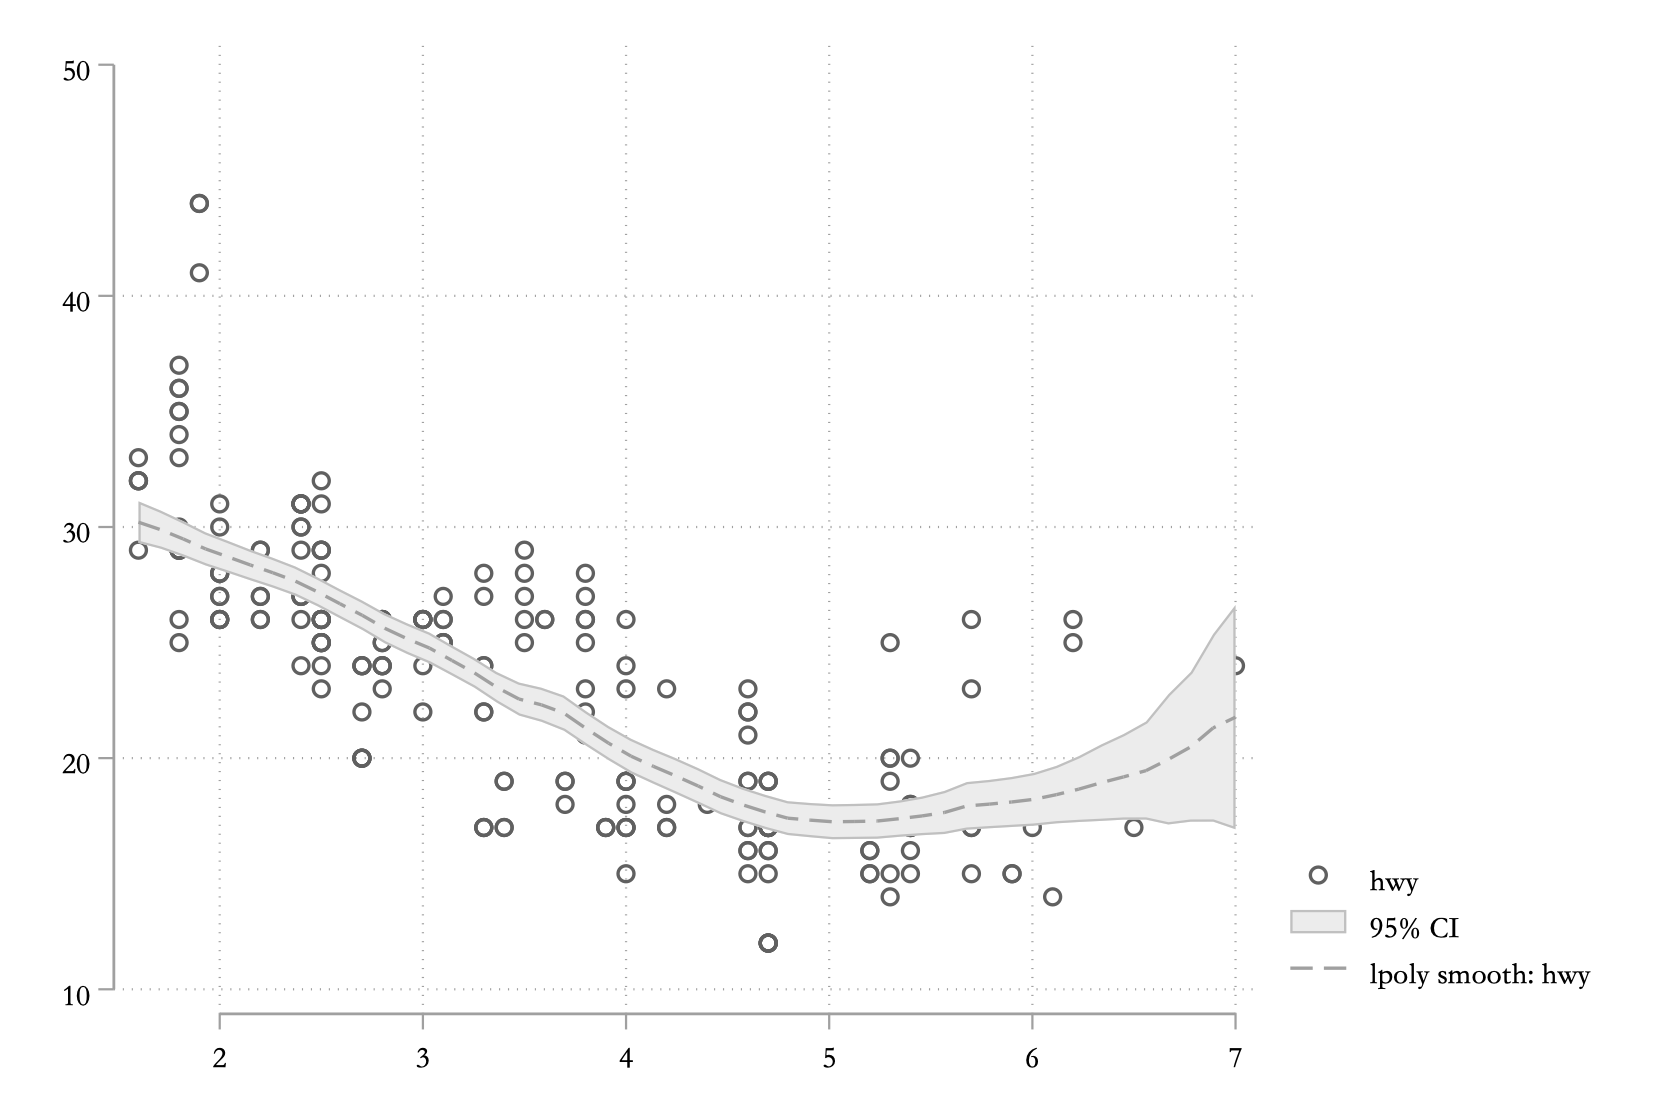
\includegraphics[width=\textwidth]{assets/lpolychwydisp.png}
    \caption{汽车排量与燃油效率的关系散点图与多项式拟合}
    \label{fig:lpolychwydisp}
  \end{figure}
\end{problem}

可以看出两个图层有着相同的x和y变量,也正是因此我们才能把这两个图层叠加在一起。但是一个是用散点表示两者的关系,一个是用多项式拟合线表示两者的关系,也就是说,两个图层使用了不同的几何对象。

人们经常会根据实际需要使用不同的几何对象表示数据,例如展示数据分布常使用直方图、箱线图,展示走势常使用线图等等。

图 \ref{fig:lpolycibydrv} 展示了针对不同的 drv 值绘制不同的曲线拟合:

\begin{lstlisting}
tw ///
lpolyci hwy displ if drv == "4", lp(solid) || ///
lpolyci hwy displ if drv == "f", lp(dash) || ///
lpolyci hwy displ if drv == "r", lp(shortdash) ||, ///
leg(order(2 "4" 4 "f" 6 "r") title(drv))
\end{lstlisting}

\begin{figure}[htbp]
  \centering
  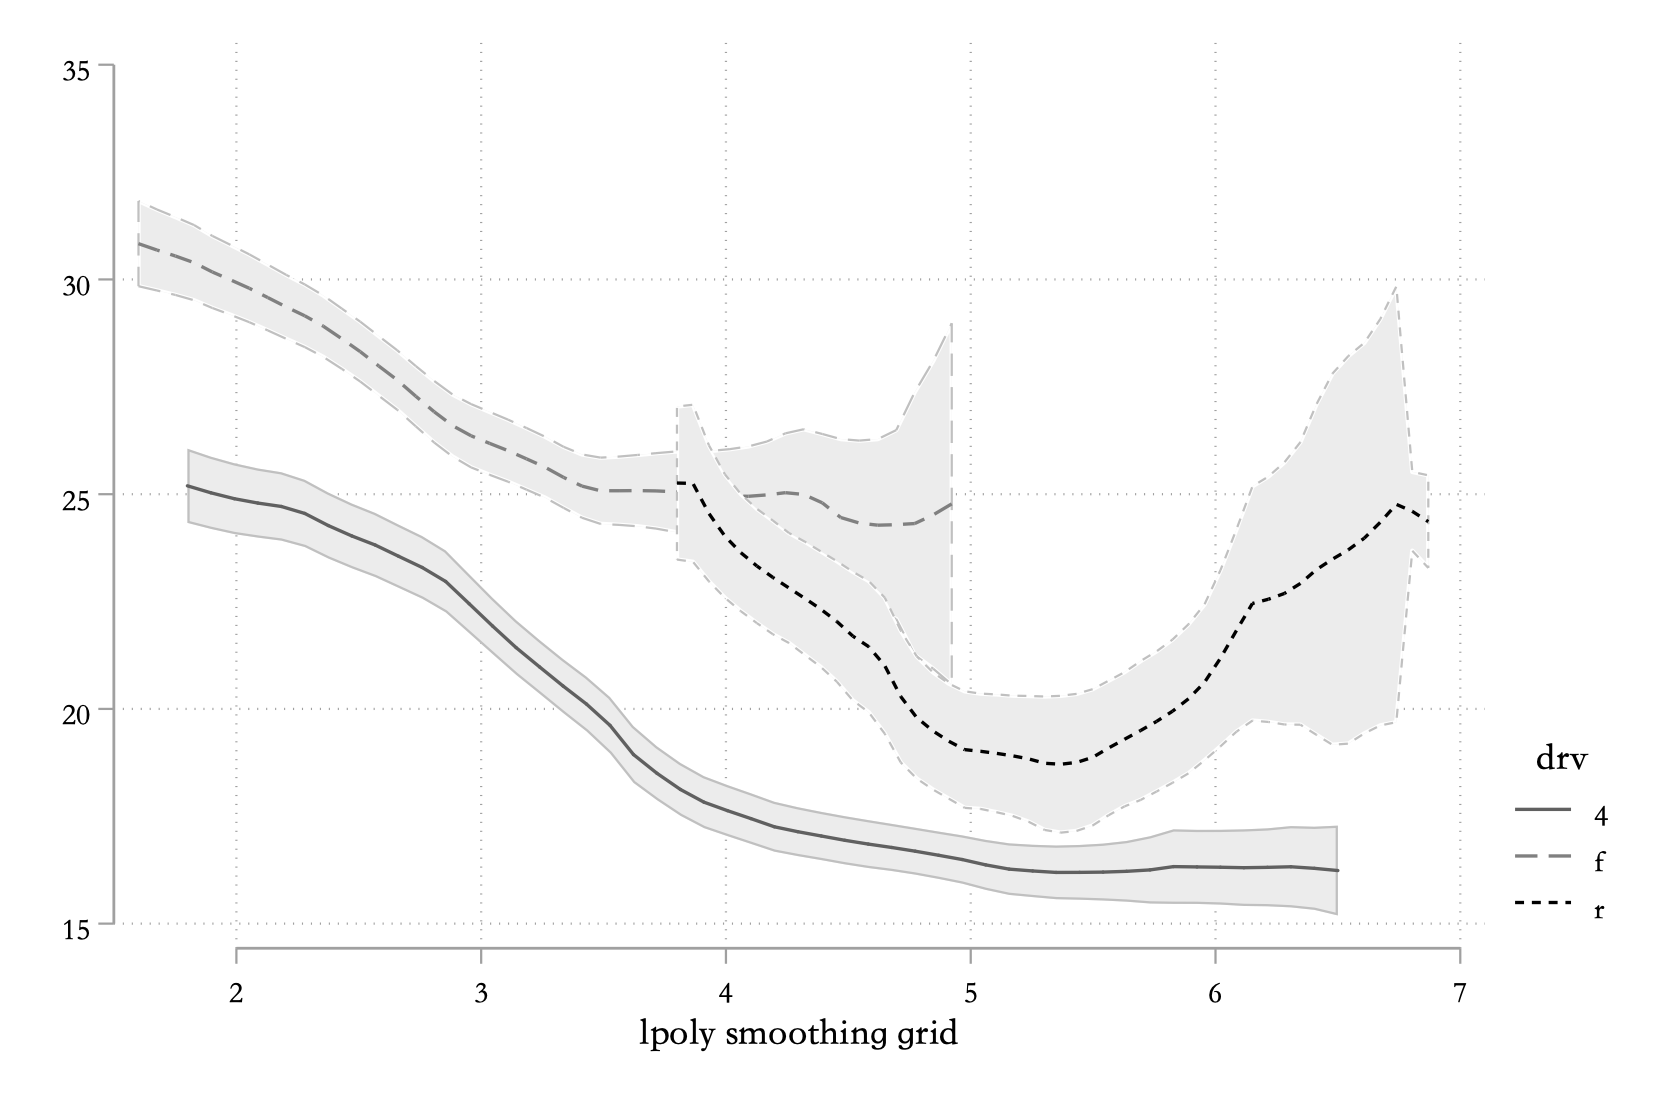
\includegraphics[width=\textwidth]{assets/lpolycibydrv.png}
  \caption{不同 drv 的汽车排量与燃油效率的关系}
  \label{fig:lpolycibydrv}
\end{figure}

这里需要补充的是,Stata中的线型有以下几种,如图 \ref{fig:linepalette}:

\begin{lstlisting}
palette linepalette
\end{lstlisting}

\begin{figure}[htbp]
  \centering 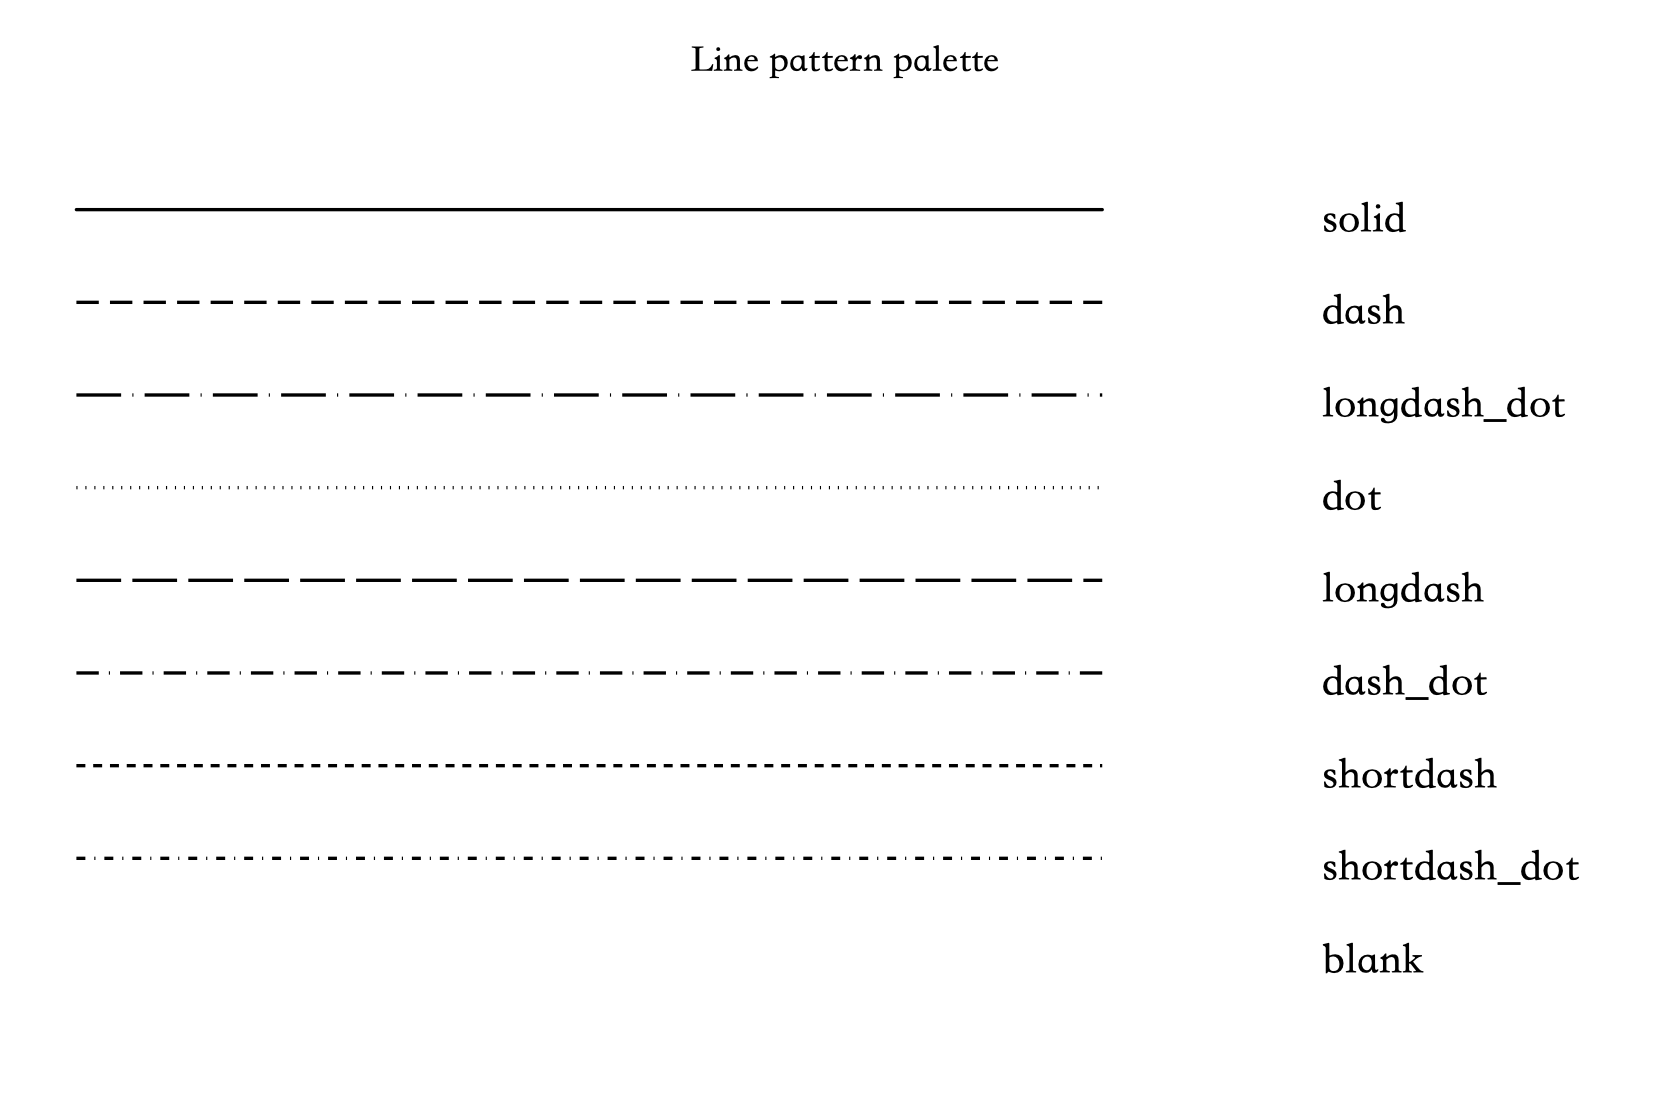
\includegraphics[width=\textwidth]{assets/linepalette.png}
  \caption{Stata 中的线型}\label{fig:linepalette}
\end{figure}

为了更容易区分,我们再对不同的图层使用不同的颜色,如图 \ref{fig:lpolycibydrv2}:

\begin{lstlisting}
colorscheme 3, palette("Set2")
return list
tw ///
lpolyci hwy displ if drv == "4", lc("`r(color1)'") || ///
lpolyci hwy displ if drv == "f", lc("`r(color2)'") || ///
lpolyci hwy displ if drv == "r", lc("`r(color3)'") || ///
sc hwy displ if drv == "4", mc("`r(color1)'") || ///
sc hwy displ if drv == "f", mc("`r(color2)'") || ///
sc hwy displ if drv == "r", mc("`r(color3)'") ||, ///
leg(order(2 "4" 4 "f" 6 "r") title(drv))
\end{lstlisting}

\begin{figure}[htbp]
  \centering 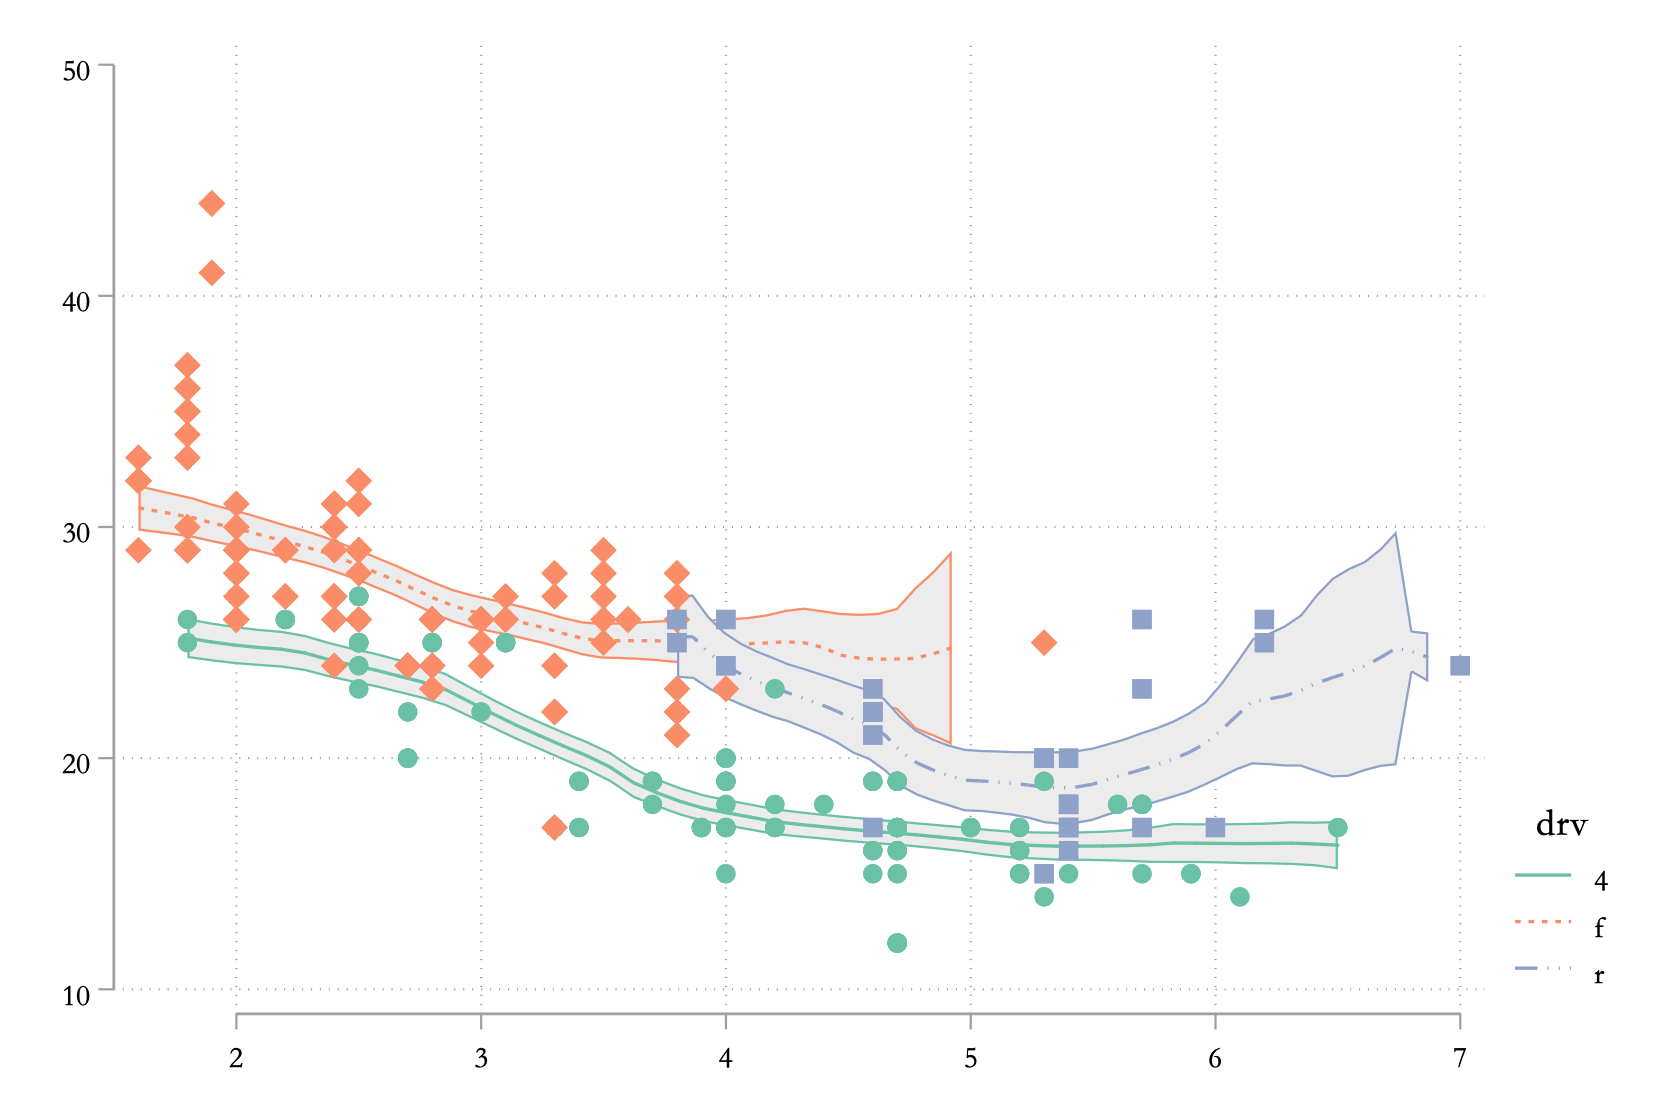
\includegraphics[width=\textwidth]{assets/lpolycibydrv2.png}
  \caption{不同 drv 的汽车排量与燃油效率的关系}
  \label{fig:lpolycibydrv2}
\end{figure}

Stata 的绘图功能是比较强大的,事实上我觉得如果一个绘图系统能够绘制不同颜色的点、线和区域,那么它就能够绘制任何图,而绘图的难易程度取决于绘图函数的设计。

图 \ref{fig:lpolycihwydispl} 展示了不同 class 的汽车排量与燃油效率的关系:

\begin{lstlisting}
colorscheme 8, palette(Set2)
tw ///
sc hwy displ if class == "2seater", mc("`r(color1)'") ms(o) || ///
sc hwy displ if class == "compact", mc("`r(color2)'") ms(o) || ///
sc hwy displ if class == "midsize", mc("`r(color3)'") ms(o) || ///
sc hwy displ if class == "minivan", mc("`r(color4)'") ms(o) || ///
sc hwy displ if class == "pickup", mc("`r(color5)'") ms(o) || ///
sc hwy displ if class == "subcompact", mc("`r(color6)'") ms(o) || ///
sc hwy displ if class == "suv", mc("`r(color7)'") ms(o) || ///
lpolyci hwy displ, lc("`r(color8)'") ||, ///
leg(order(1 "2seater" ///
          2 "compact" ///
          3 "midsize" ///
          4 "minivan" ///
          5 "pickup" ///
          6 "subcompact" ///
          7 "suv") title(class))
\end{lstlisting}

\begin{figure}[htbp]
  \centering
  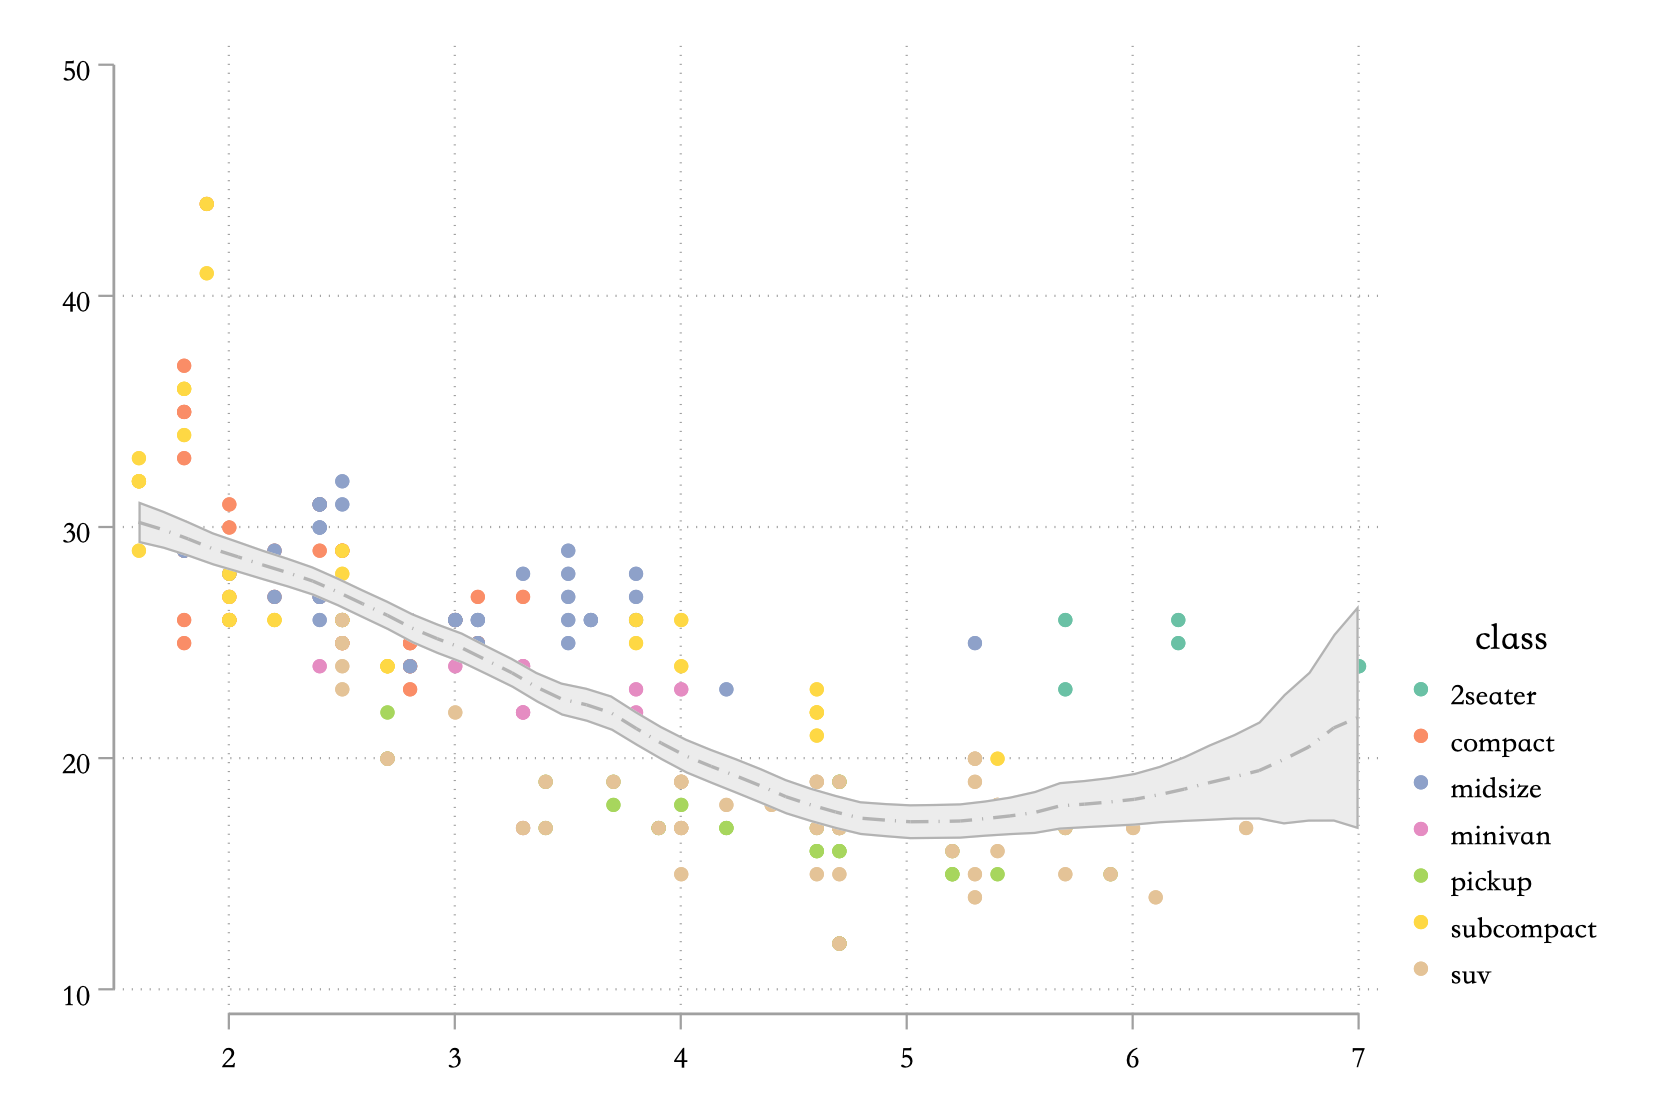
\includegraphics[width=\textwidth]{assets/lpolycihwydispl.png}
  \caption{不同 class 的汽车排量与燃油效率的关系}\label{fig:lpolycihwydispl}
\end{figure}

当然也可以对 class 的一个子集进行多项式拟合,如图 \ref{fig:lpolycihwydispl2}:

\begin{lstlisting}
colorscheme 8, palette(Set2)
tw ///
sc hwy displ if class == "2seater", mc("`r(color1)'") ms(o) || ///
sc hwy displ if class == "compact", mc("`r(color2)'") ms(o) || ///
sc hwy displ if class == "midsize", mc("`r(color3)'") ms(o) || ///
sc hwy displ if class == "minivan", mc("`r(color4)'") ms(o) || ///
sc hwy displ if class == "pickup", mc("`r(color5)'") ms(o) || ///
sc hwy displ if class == "subcompact", mc("`r(color6)'") ms(o) || ///
sc hwy displ if class == "suv", mc("`r(color7)'") ms(o) || ///
lpolyci hwy displ if class == "subcompact", lc("`r(color8)'") ||, ///
leg(order(1 "2seater" ///
          2 "compact" ///
          3 "midsize" ///
          4 "minivan" ///
          5 "pickup" ///
          6 "subcompact" ///
          7 "suv") title(class))
\end{lstlisting}

\begin{figure}[htbp]
  \centering
  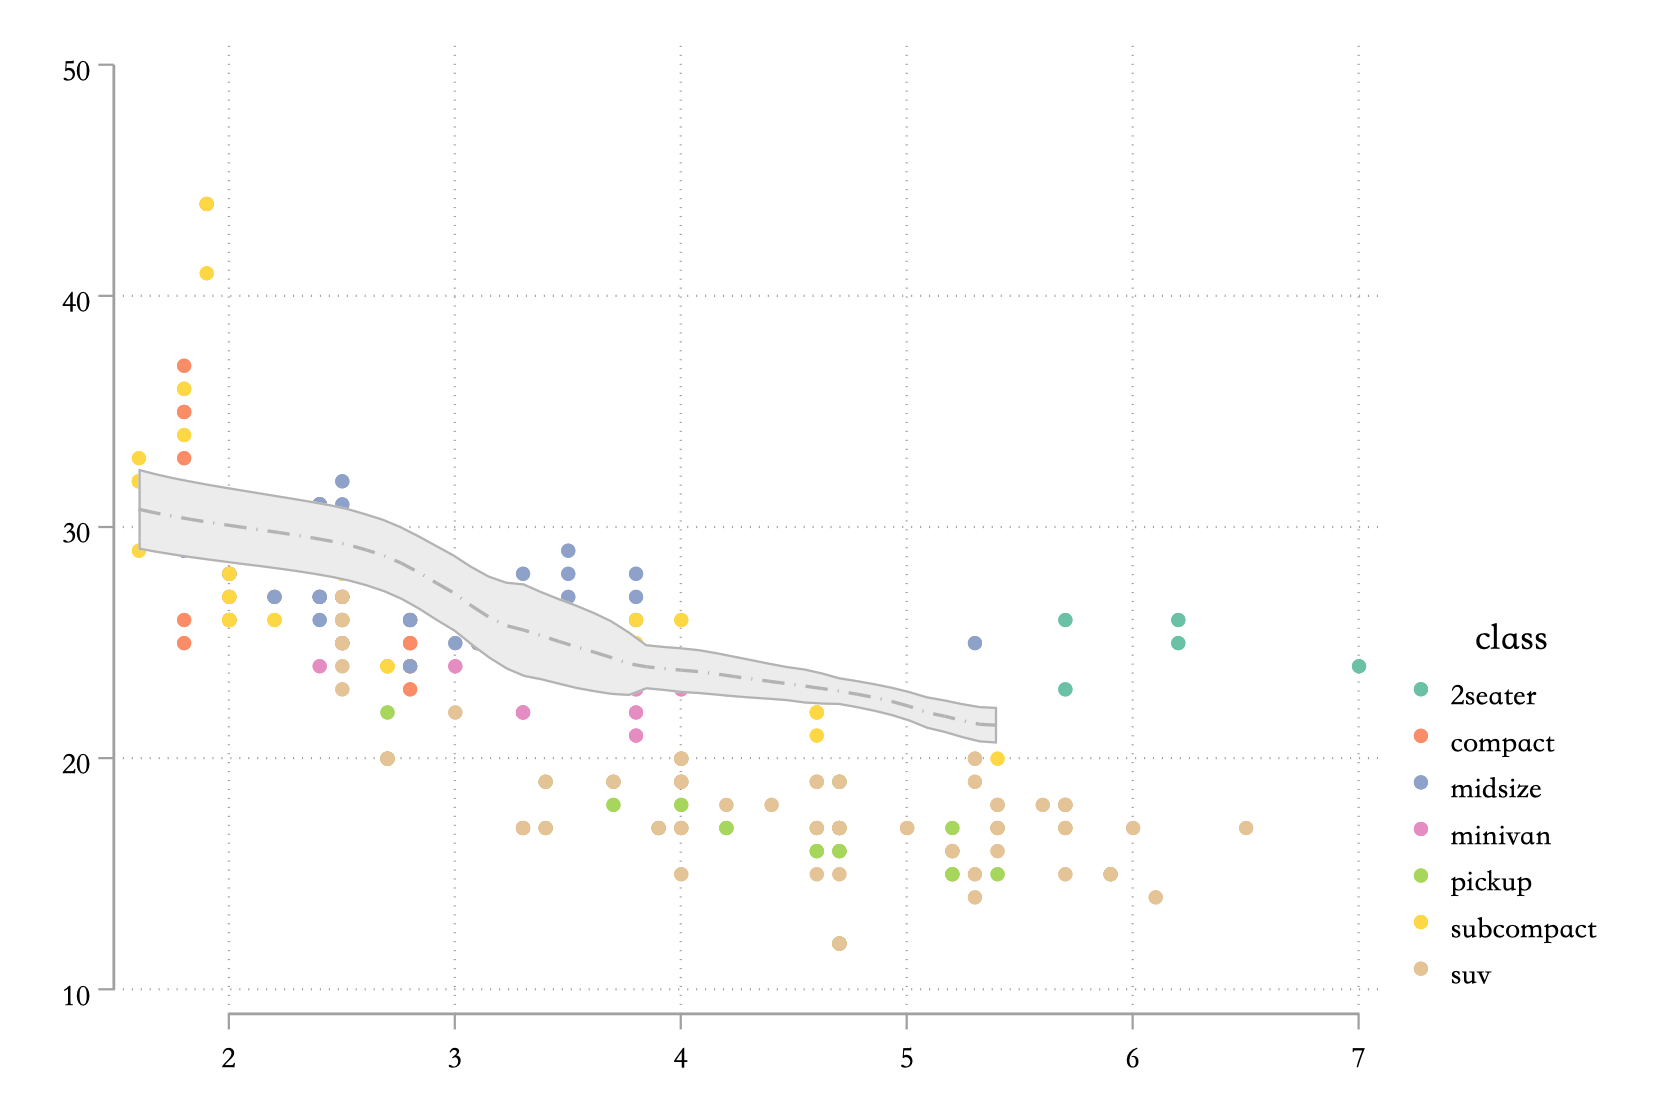
\includegraphics[width=\textwidth]{assets/lpolycihwydispl2.png}
  \caption{不同 class 的汽车排量与燃油效率的关系}
  \label{fig:lpolycihwydispl2}
\end{figure}

\section{统计变换}

Stata 绘制直方图的命令是 \texttt{histogram} ,简写为 \texttt{hist},如图 \ref{fig:histcut}:

\begin{lstlisting}
sysuse diamonds, clear
hist cut, barwidth(0.8) xlab(, val) freq
\end{lstlisting}

\begin{figure}[htbp]
  \centering
  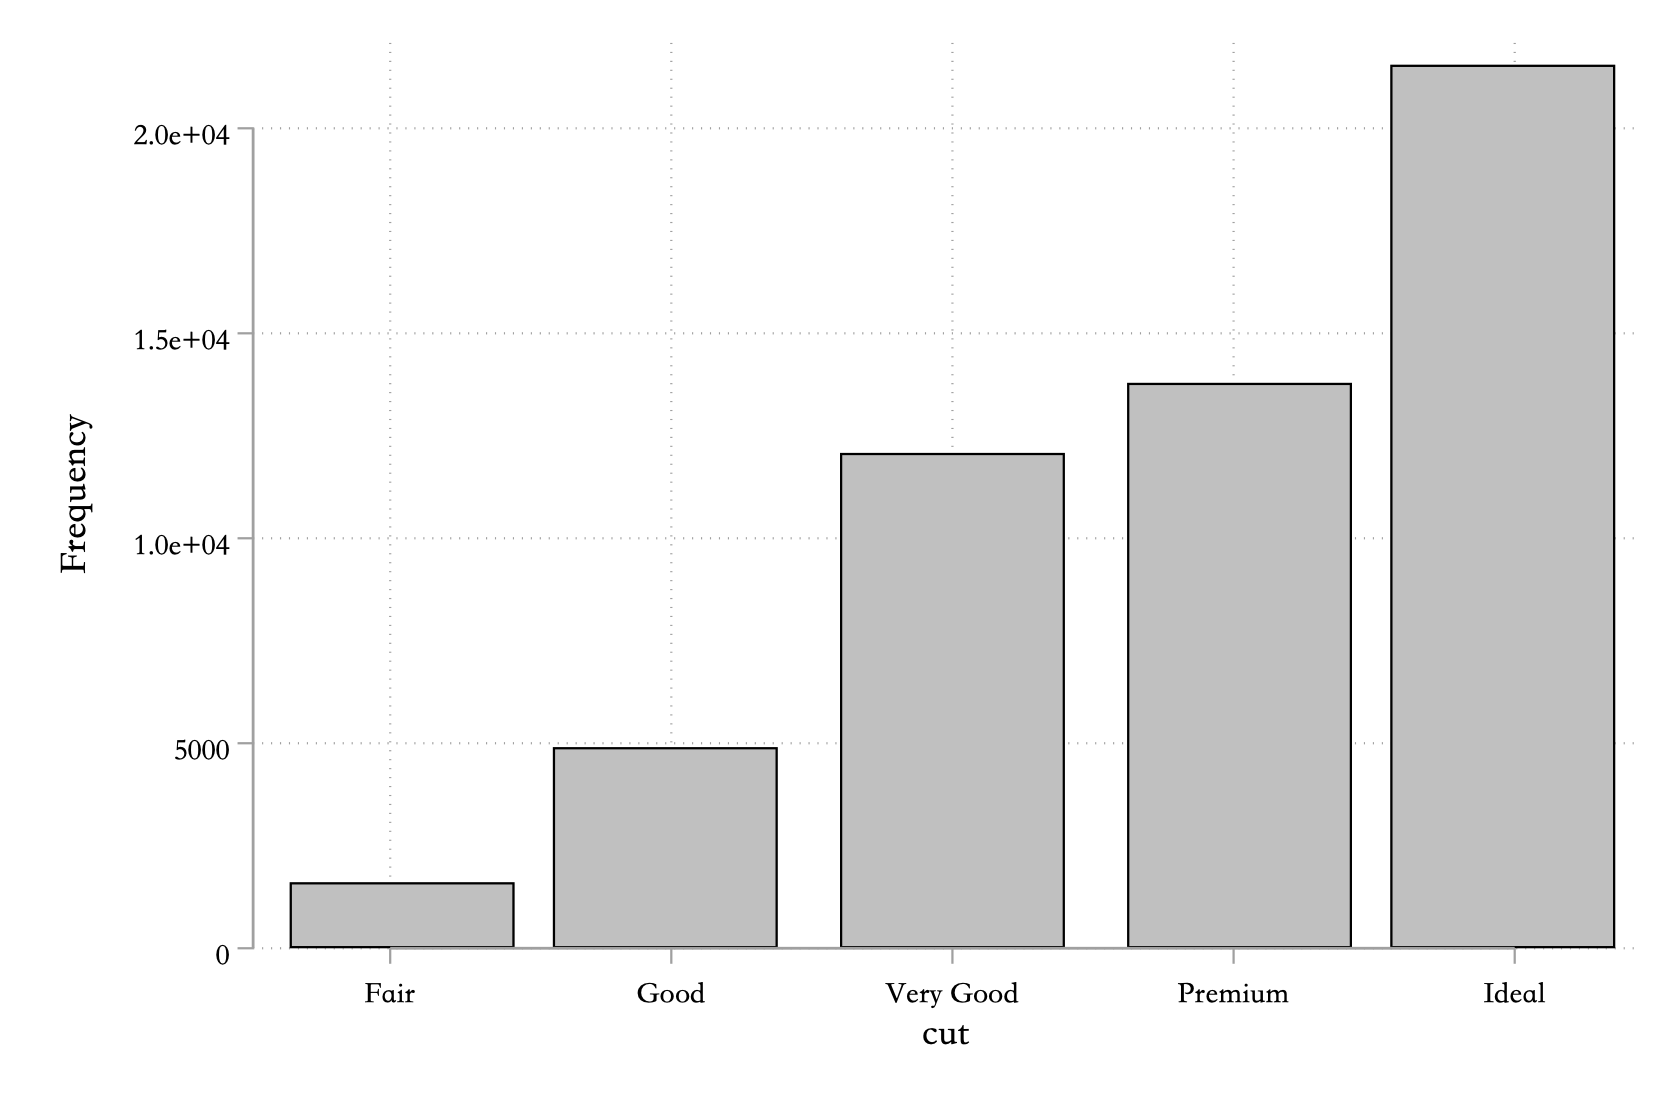
\includegraphics[width=0.8\textwidth]{assets/histcut.png}
  \caption{钻石切工分布直方图}\label{fig:histcut}
\end{figure}

我们可以注意到,图 \ref{fig:histcut} 中的横轴是 cut 变量,纵轴是 cut 变量各个取值的分布,而我们主要到数据集中是没有这个变量的,显然这个变量是 hist 命令计算过程中生成的,下面的语句展示了如何对 cut 变量的各个取值进行计数然后绘制直方图,如图 \ref{fig:barcut}:

\begin{lstlisting}
contract cut
tw bar _freq cut, barwidth(0.8) xlab(, val)
\end{lstlisting}

\begin{figure}[htbp]
  \centering
  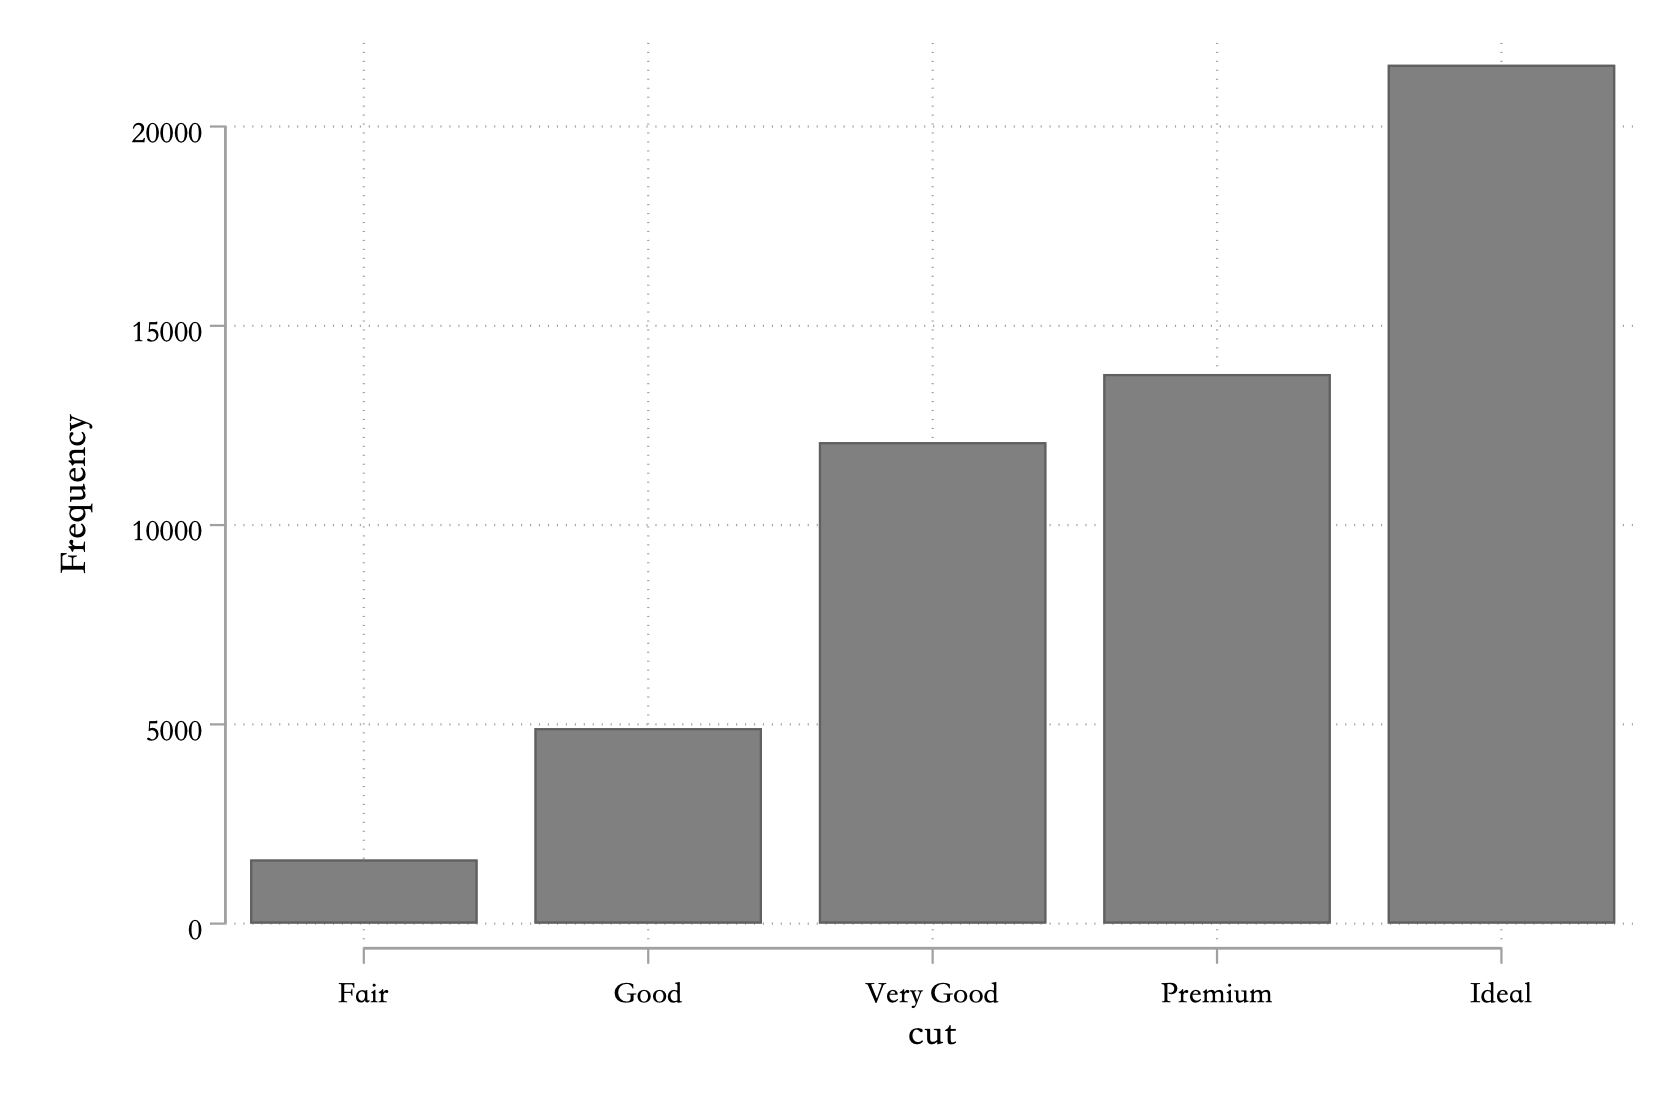
\includegraphics[width=\textwidth]{assets/barcut.png}
  \caption{钻石切工分布直方图}\label{fig:barcut}
\end{figure}

contract 命令能够快速的对变量进行计数,详细用法可以参考其帮助文档(help contract)或者我的博客文章: \href{https://www.czxa.top/posts/1170/\#contract\%E5\%91\%BD\%E4\%BB\%A4}{Stata旧笔记整理(八)\#contract命令}。

contract 命令运行之后会生成一个新的数据集,如表 \ref{tab:cut}:

\begin{table}[htbp]
\caption{\label{tab:cut}contract cut 的结果}
\centering
\begin{tabular}{lr}
\toprule
cut & \_freq\\
\midrule
Fair & 1610\\
Good & 4906\\
Very Good & 12082\\
Premium & 13791\\
Ideal & 21551\\
\bottomrule
\end{tabular}
\end{table}

通过这个过程你就会发现所谓的 \textcolor{third3}{统计变换} 不过就是把一系列的计算过程封装在命令中,并不难懂。

\texttt{hist} 命令的纵轴也可以为频率(Density),去掉 freq 选项即可,如图 \ref{fig:histcut2}:

\begin{lstlisting}
sysuse diamonds, clear
hist cut, barwidth(0.8) xlab(, val)
\end{lstlisting}

\begin{figure}[htbp]
  \centering 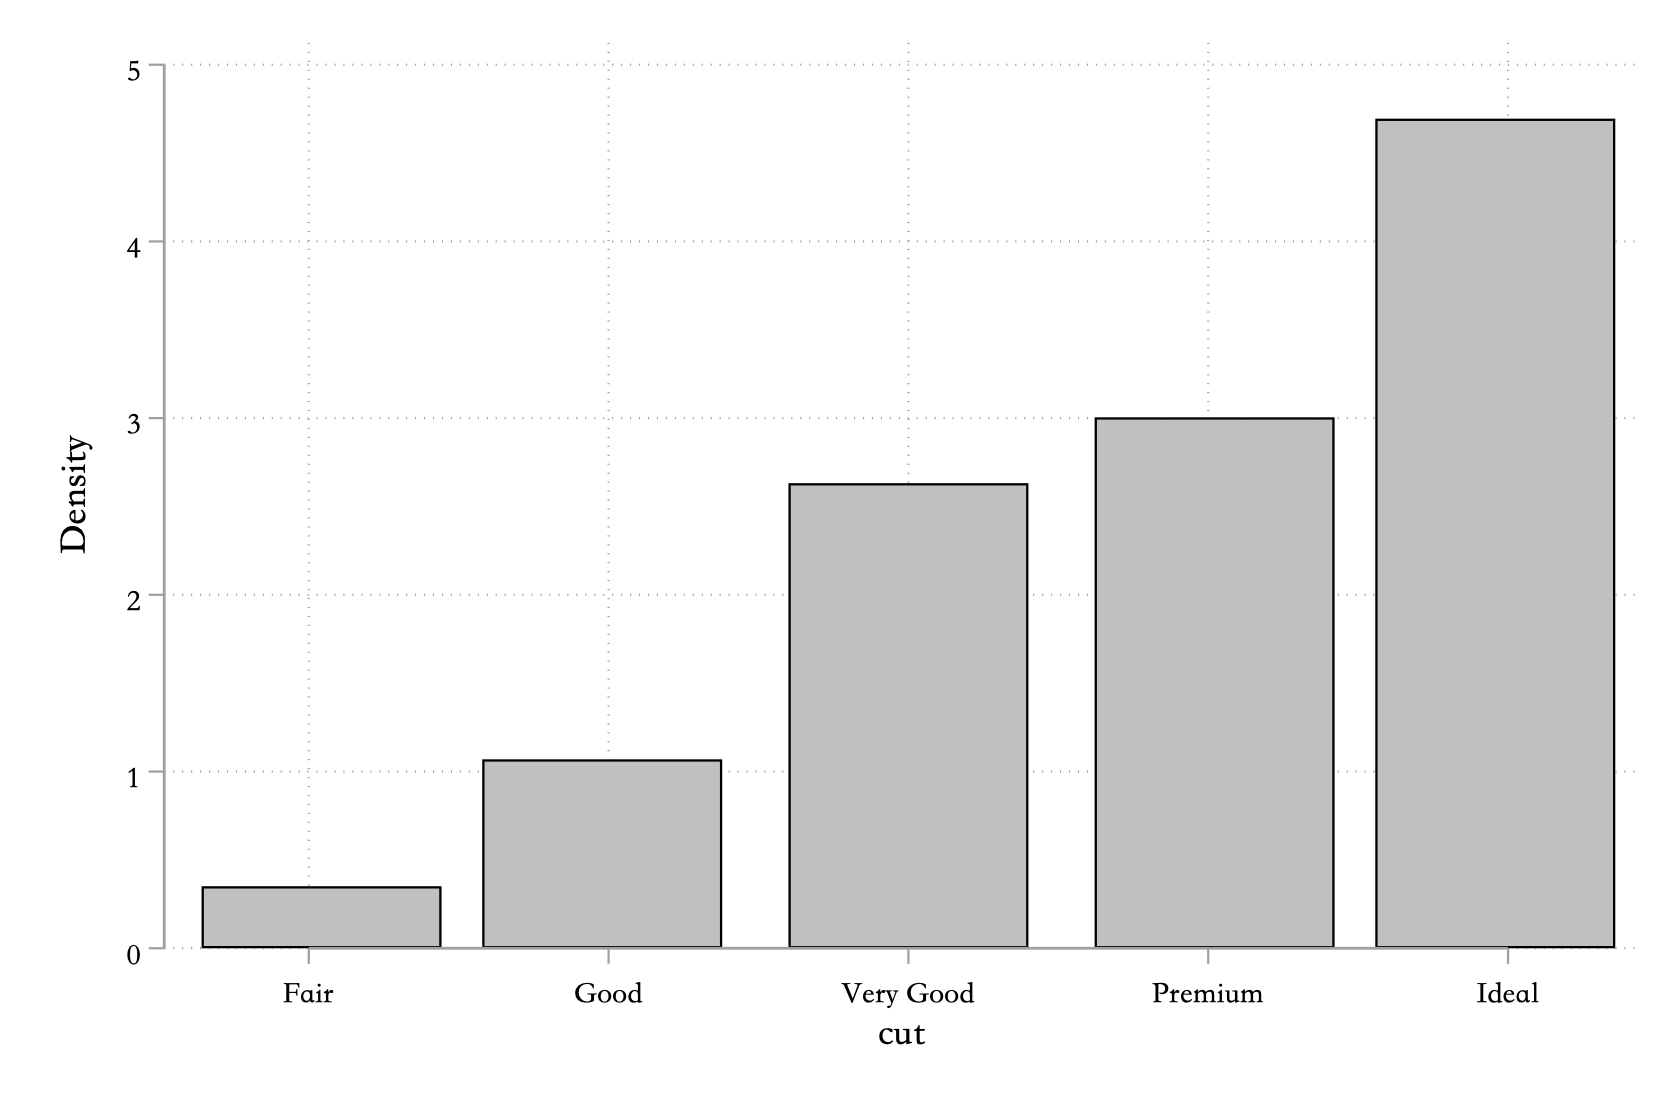
\includegraphics[width=\textwidth]{assets/histcut2.png}
  \caption{钻石切工分布直方图}\label{fig:histcut2}
\end{figure}

统计变换经常是件苦力活,因为很多时候我们需要先计算我们需要进行的统计变换,然后再把变换后的结果整理好读入Stata再绘图,\lstinline{collapse} 是一个非常好用的命令,可以帮我们简化这个过程,例如我想展示不同cut值depth变量的范围和中位数:

\begin{lstlisting}
sysuse diamonds, clear
collapse    (min) depthmin = depth ///
            (median) depthmedian = depth ///
            (max) depthmax = depth, by(cut)
\end{lstlisting}

这个时候得到的结果见表 \ref{tab:depthmmm}:

\begin{table}[htbp]
\caption{\label{tab:depthmmm}collapse depth 的结果}
\centering
\begin{tabular}{lrrr}
\toprule
cut & depthmin & depthmedian & depthmax\\
\midrule
Fair & 43.0 & 65.0 & 79.0\\
Good & 54.3 & 63.4 & 67.0\\
Very Good & 56.8 & 62.1 & 64.9\\
Premium & 58.0 & 61.4 & 63.0\\
Ideal & 43.0 & 61.8 & 66.7\\
\bottomrule
\end{tabular}
\end{table}

然后我们再绘图,绘图结果见图 \ref{fig:depth3m}:

\begin{lstlisting}
tw ///
rspike depthmax depthmin cut || ///
sc depthmedian cut, xlab(, val) ms(O) mc(black) ||, ///
leg(off)
\end{lstlisting}

\begin{figure}[htbp]
  \centering 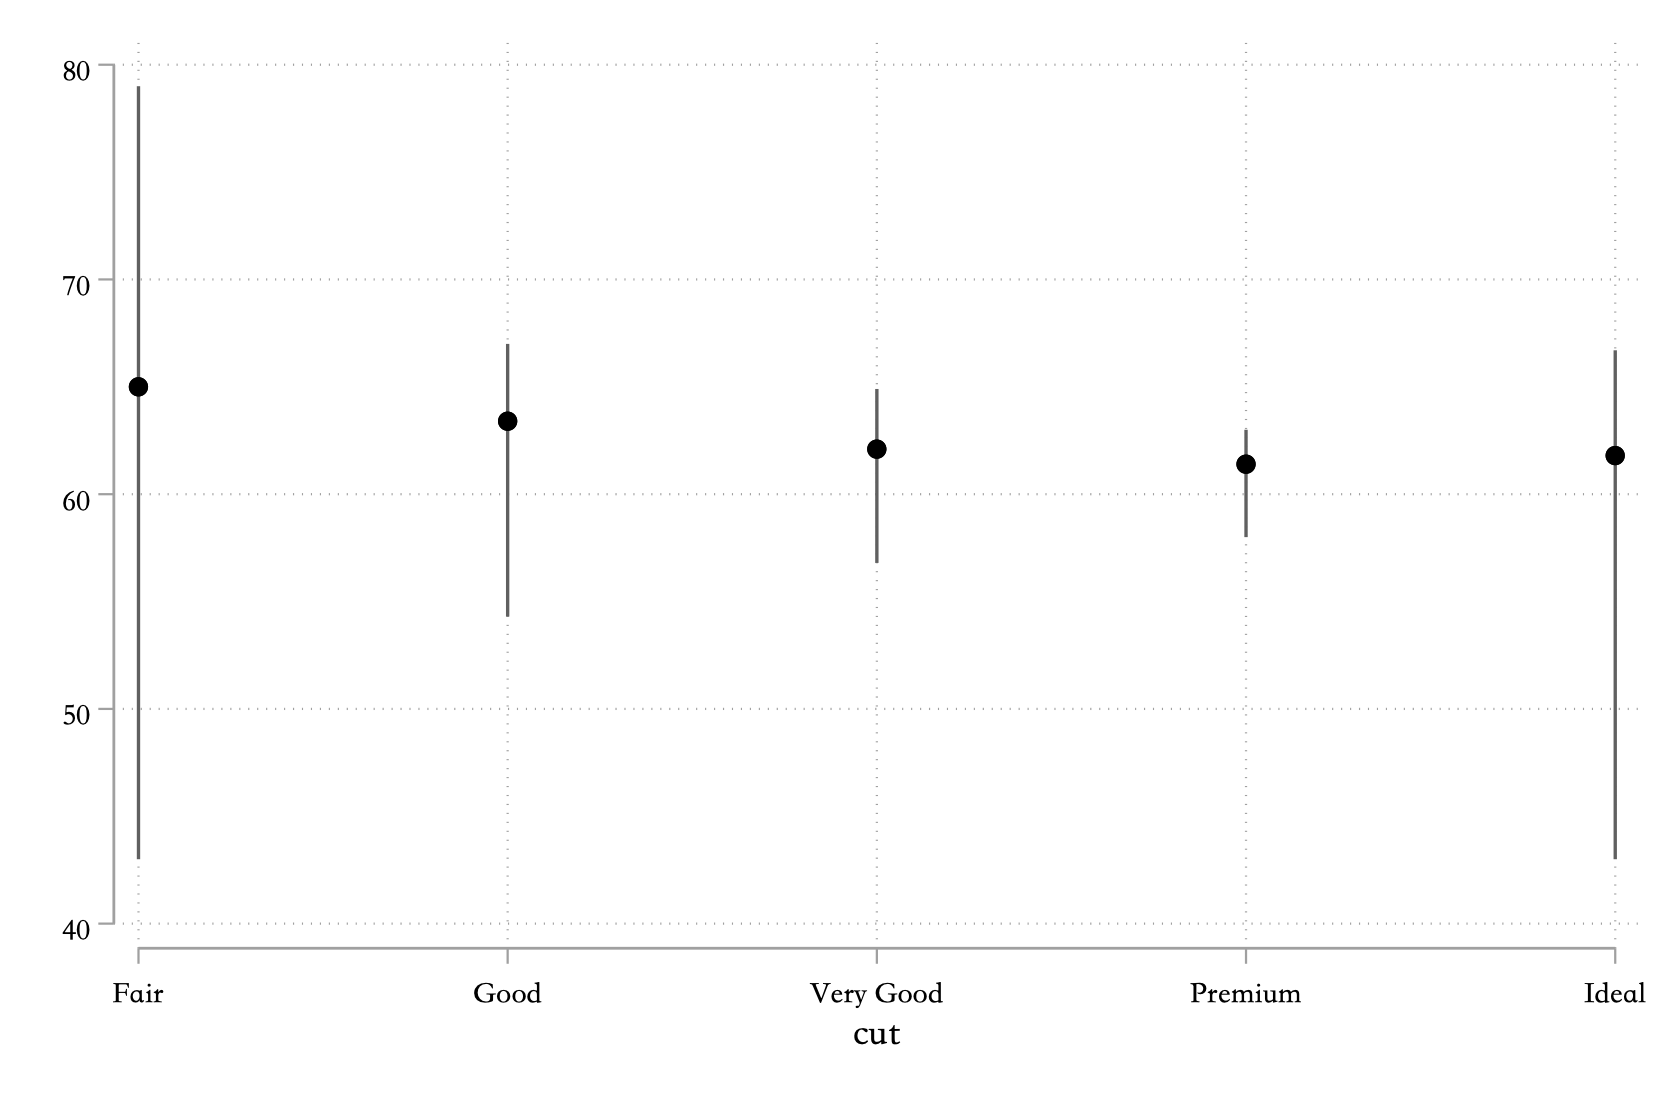
\includegraphics[width=\textwidth]{assets/depth3m.png}
  \caption{钻石深度的分布}
  \label{fig:depth3m}
\end{figure}

\section{位置调整}

通过不同的颜色设置,我们可以得到下面的图 \ref{fig:barcutmulticolor} 和图 \ref{fig:barcutmulticolor2}:

\begin{lstlisting}
sysuse diamonds, clear
contract cut
colorscheme 5, palette(Set2)
tw ///
bar _freq cut if cut == 1, fc("`r(color1)'") barwidth(0.8) || ///
bar _freq cut if cut == 2, fc("`r(color2)'") barwidth(0.8) || ///
bar _freq cut if cut == 3, fc("`r(color3)'") barwidth(0.8) || ///
bar _freq cut if cut == 4, fc("`r(color4)'") barwidth(0.8) || ///
bar _freq cut if cut == 5, fc("`r(color5)'") ///
barwidth(0.8) xlab(, val) leg(off)
\end{lstlisting}

\begin{figure}[htbp]
  \centering
  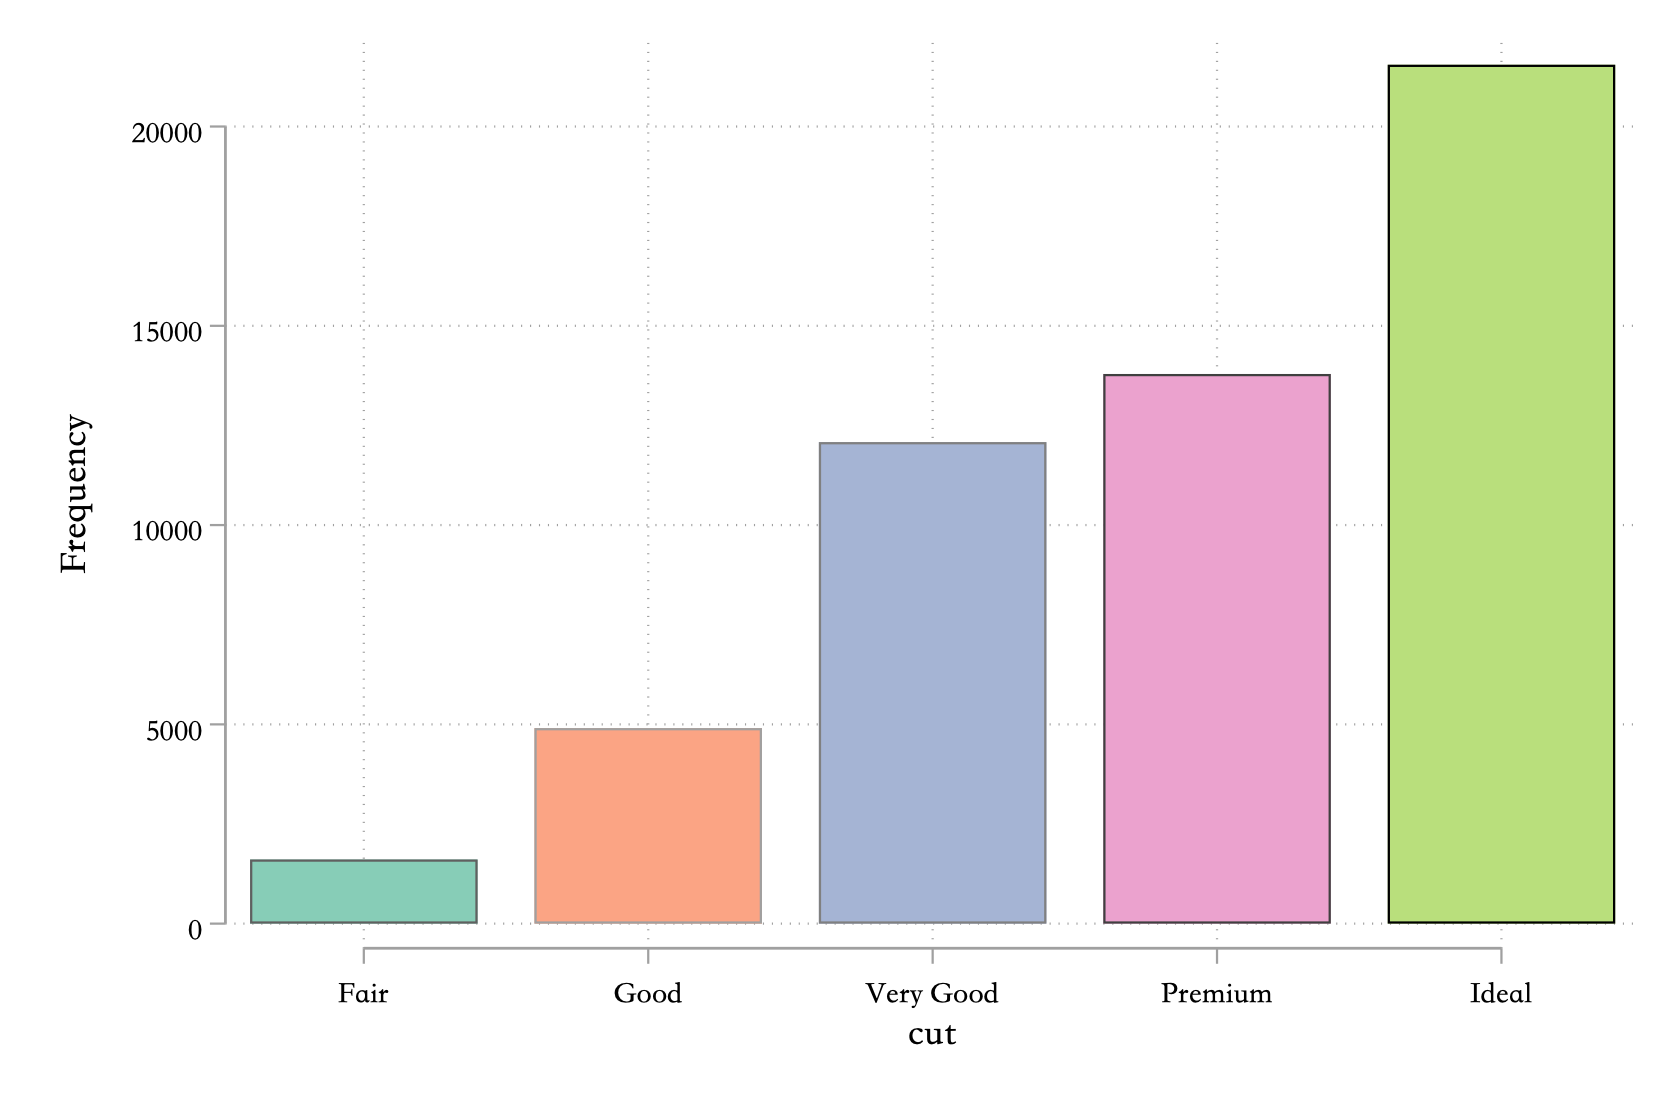
\includegraphics[width=\textwidth]{assets/barcutmulticolor.png}
  \caption{钻石切工的分布}\label{fig:barcutmulticolor}
\end{figure}

\begin{lstlisting}
sysuse diamonds, clear
contract cut
colorscheme 5, palette(Set1)
tw ///
bar _freq cut if cut == 1, lc("`r(color1)'") barwidth(0.8) || ///
bar _freq cut if cut == 2, lc("`r(color2)'") barwidth(0.8) || ///
bar _freq cut if cut == 3, lc("`r(color3)'") barwidth(0.8) || ///
bar _freq cut if cut == 4, lc("`r(color4)'") barwidth(0.8) || ///
bar _freq cut if cut == 5, lc("`r(color5)'") ///
barwidth(0.8) xlab(, val) leg(off)
\end{lstlisting}

\begin{figure}[htbp]
  \centering
  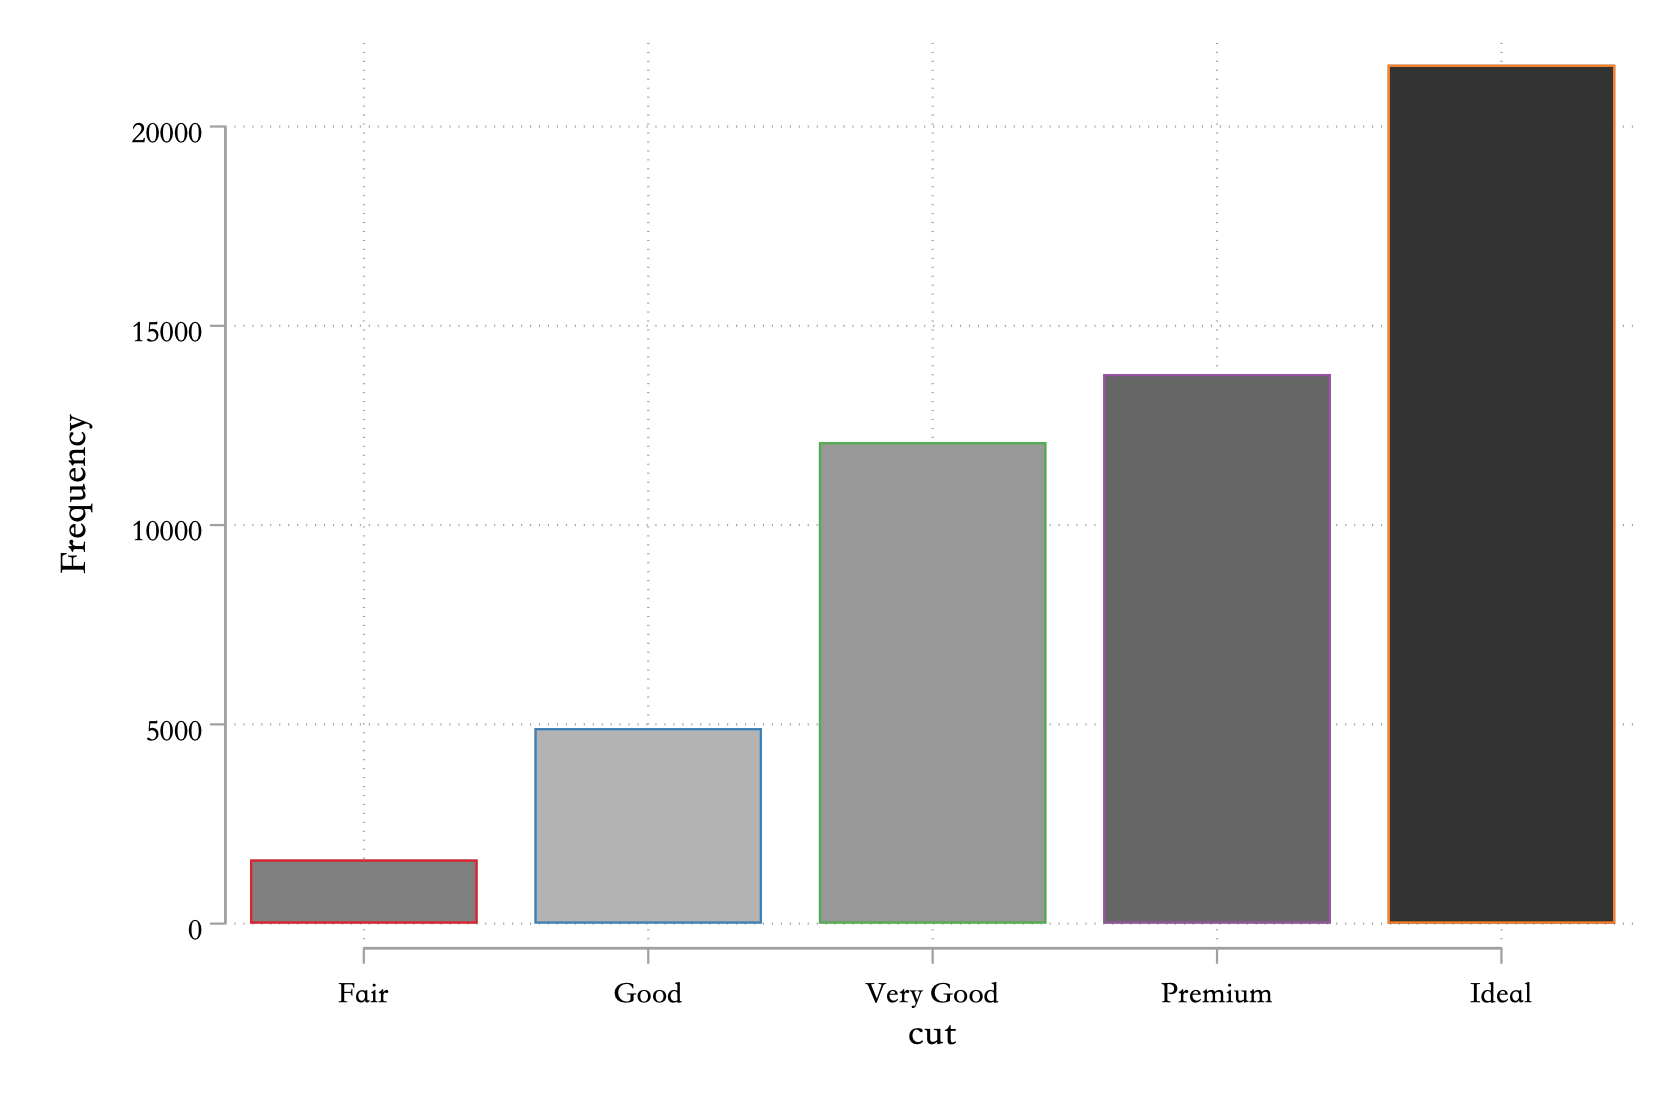
\includegraphics[width=\textwidth]{assets/barcutmulticolor2.png}
  \caption{钻石切工的分布}
  \label{fig:barcutmulticolor2}
\end{figure}

两幅图的区别就在于,第一幅图是使用 \texttt{fc()} 选项,这个选项控制对直方条的填充色,第二幅图使用的是 \texttt{lc()} 选项,这个选项控制直方条边缘的颜色。

实际上,上面两幅图关于颜色的设置都是没有什么实际意义的,只是让图看起来更加炫酷。但是有时候我们想知道例如``我们班的男生和女生生源地分布''这种问题的答案,这个时候使用颜色填充就有意义了,例如图 \ref{fig:stackcutclarity}钻石不同切工的克拉分布:

\begin{lstlisting}
sysuse diamonds, clear
colorscheme 8, palette(Paired)
gr bar, over(clarity) over(cut) ///
    stack asyvars yti(count) ///
    leg(ti(clarity)) ///
    bar(1, color("`r(color1)'")) ///
    bar(2, color("`r(color2)'")) ///
    bar(3, color("`r(color3)'")) ///
    bar(4, color("`r(color4)'")) ///
    bar(5, color("`r(color5)'")) ///
    bar(6, color("`r(color6)'")) ///
    bar(7, color("`r(color7)'")) ///
    bar(8, color("`r(color8)'"))
\end{lstlisting}

\begin{figure}[htbp]
  \centering
  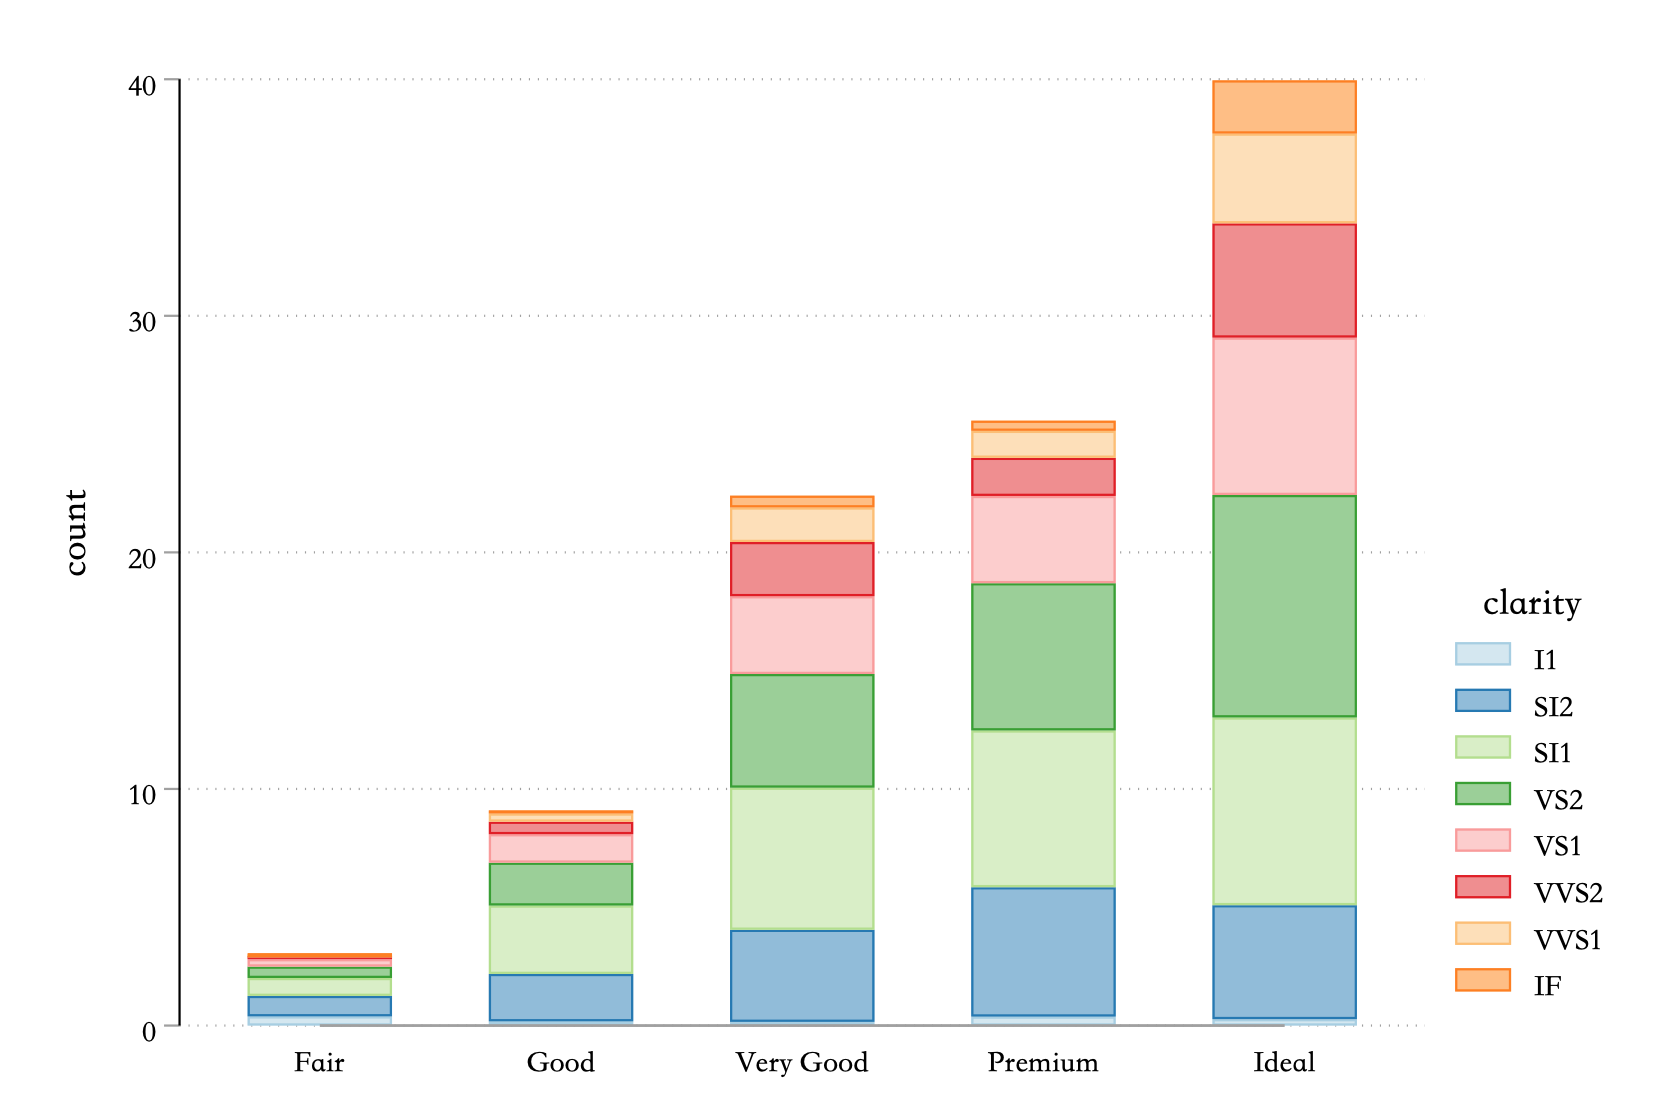
\includegraphics[width=\textwidth]{assets/stackcutclarity.png}
  \caption{钻石不同切工的克拉分布}\label{fig:stackcutclarity}
\end{figure}

有时候我们会绘制图 \ref{fig:histautoprice}:

\begin{lstlisting}
sysuse auto, clear
tw ///
hist price if for || ///
hist price if !for
\end{lstlisting}

\begin{figure}[htbp]
  \centering 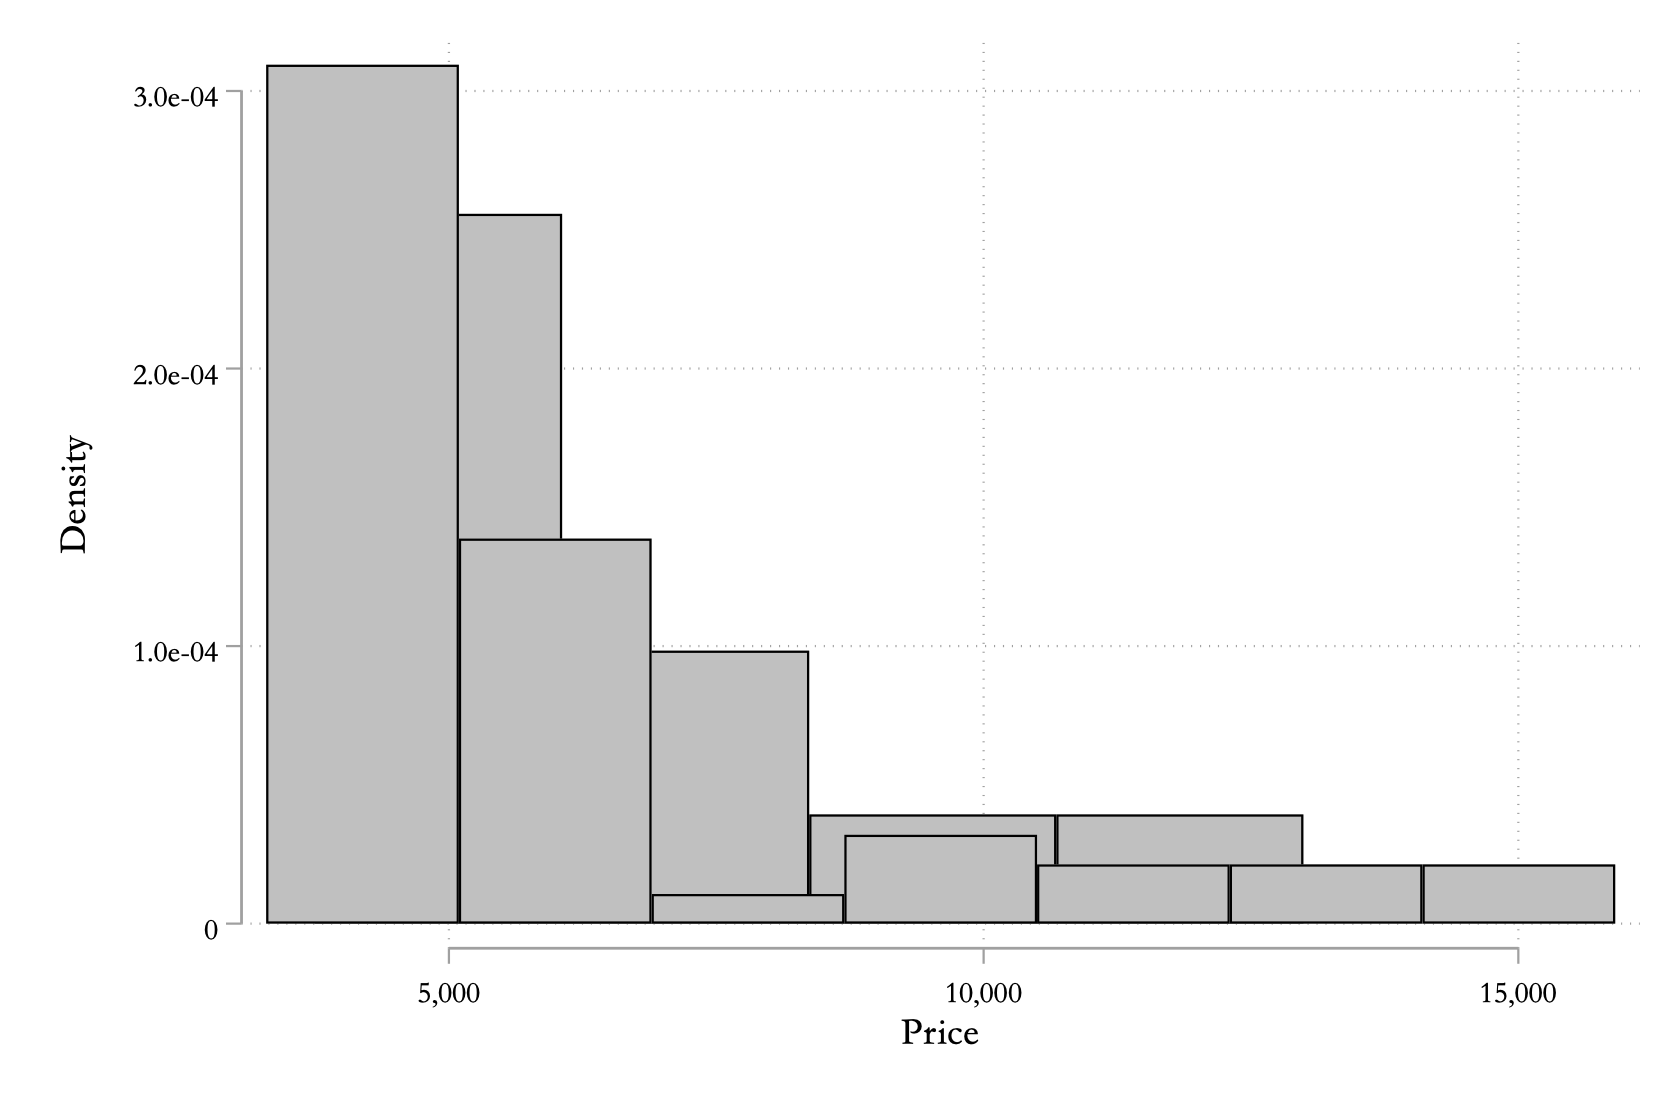
\includegraphics[width=0.8\textwidth]{assets/histautoprice.png}
  \caption{国产车和进口车的价格分布}\label{fig:histautoprice}
\end{figure}

这个图的问题就是相互重叠问题很严重,为此我们可以采取下面两种方法解决这个问题,第一种是将位于上层的图层设置为透明的,如图 \ref{fig:histautoprice2}:

\begin{lstlisting}
tw ///
hist price if for, fc(red) || ///
hist price if !for, fc(green%50) ///
    leg(order(1 "进口车" 2 "国产车"))
\end{lstlisting}

\begin{figure}[htbp]
  \centering
  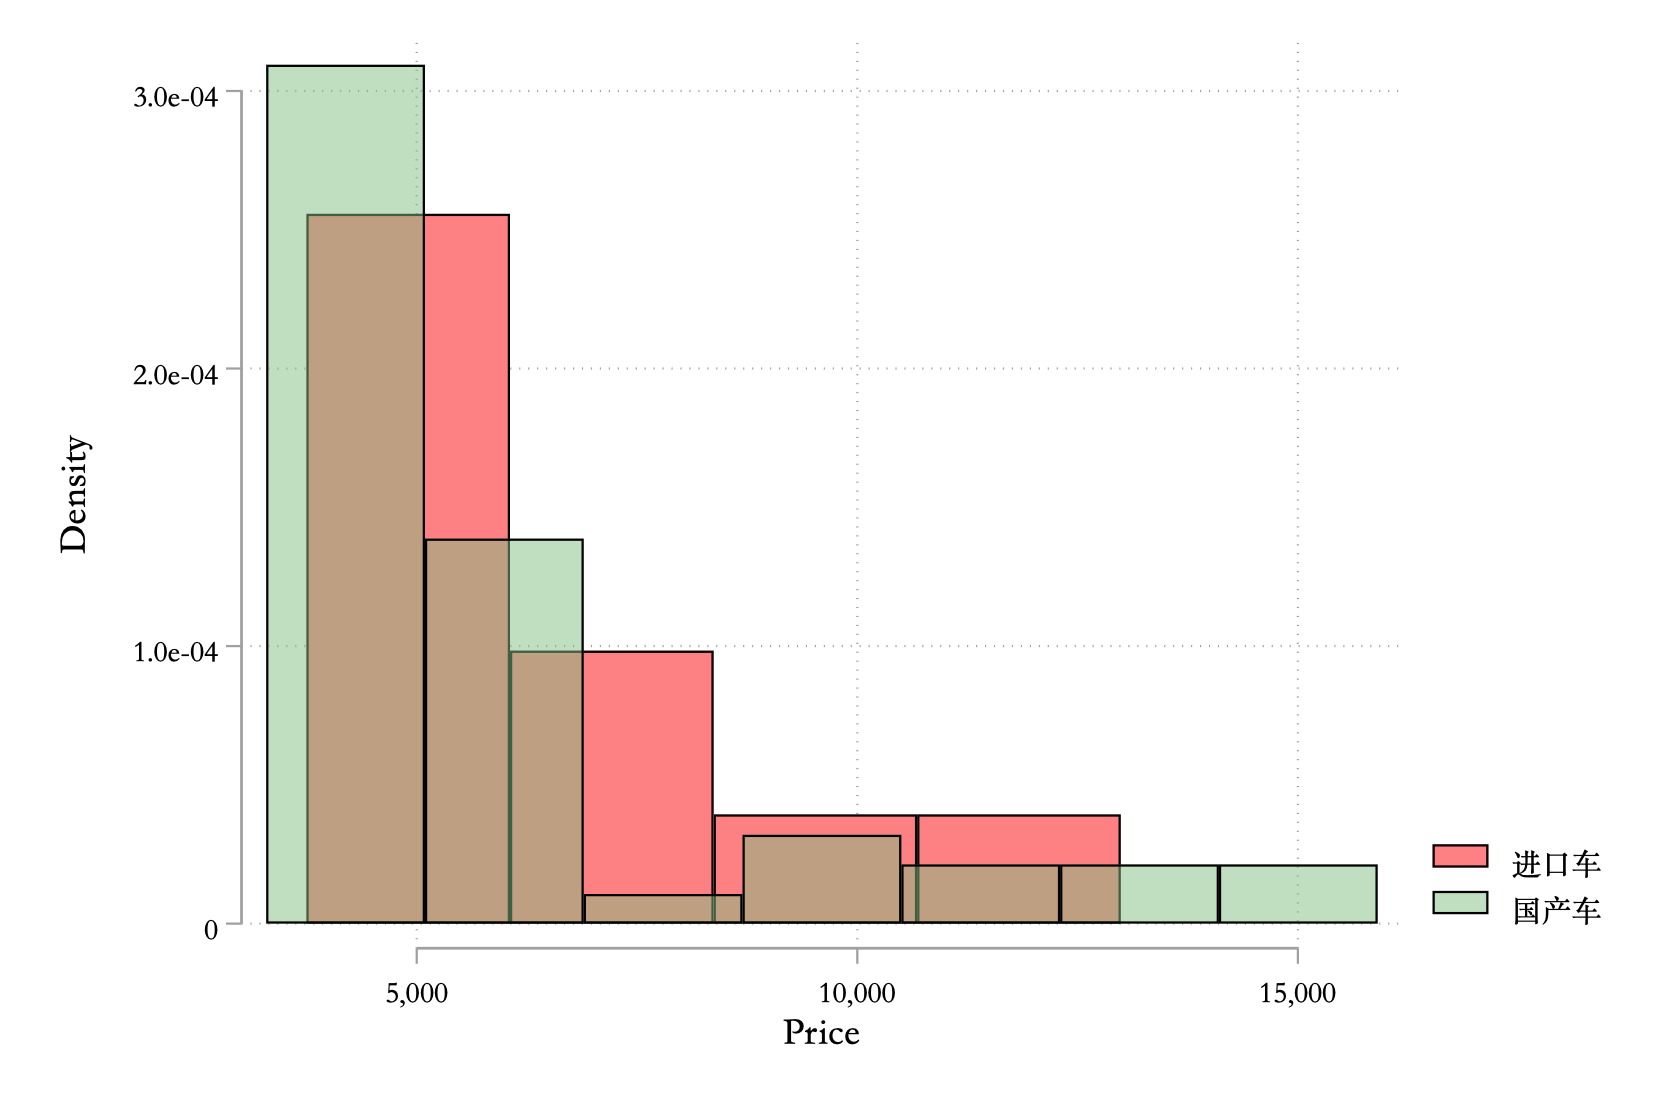
\includegraphics[width=\textwidth]{assets/histautoprice2.png}
  \caption{国产车和进口车的价格分布}\label{fig:histautoprice2}
\end{figure}

第二种方法是不再给柱形图填充颜色,如图 \ref{fig:histautoprice3}:

\begin{lstlisting}
tw ///
hist price if for, fc(red) lc(red) || ///
hist price if !for, color(none) lc(green) ///
    leg(order(1 "进口车" 2 "国产车"))
\end{lstlisting}

\begin{figure}[htbp]
  \centering 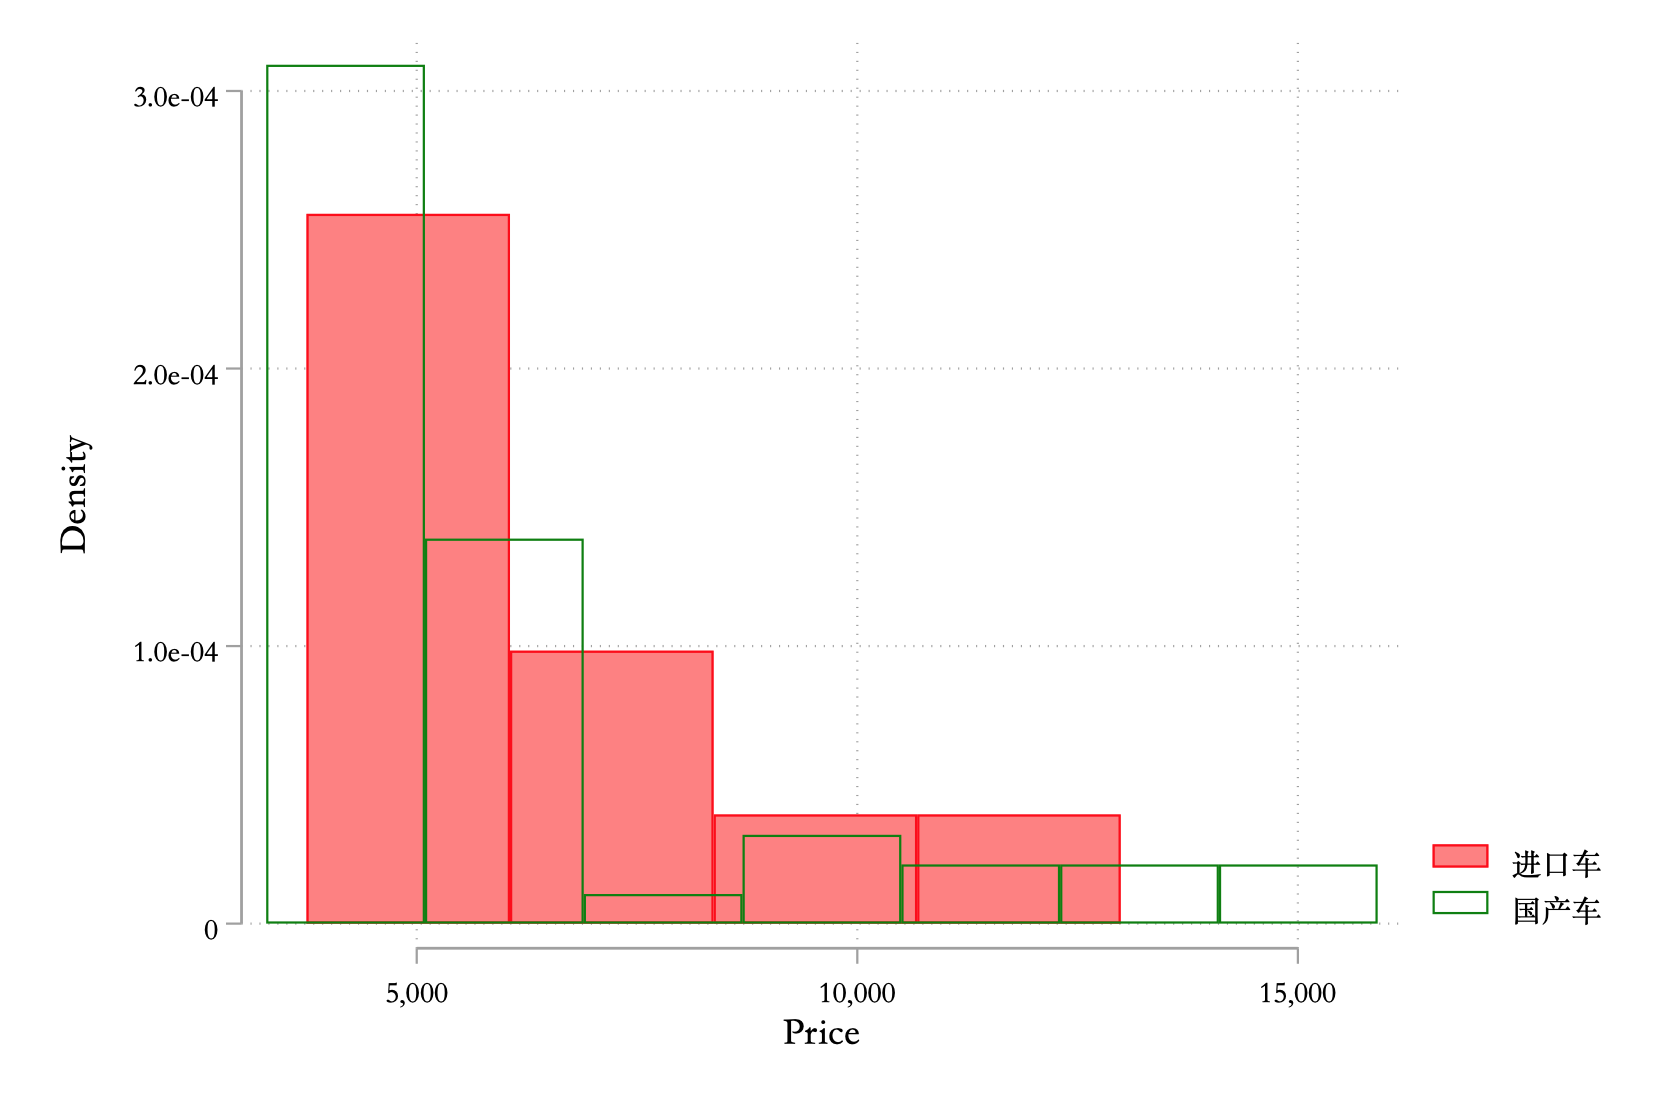
\includegraphics[width=\textwidth]{assets/histautoprice3.png}
  \caption{国产车和进口车的价格分布}\label{fig:histautoprice3}
\end{figure}

位置调整有三种,用 ggplot2 的话来说,分别是 \textcolor{third2}{identity}、\textcolor{third2}{fill} 和 \textcolor{third2}{dodge}。刚刚绘制的图 \ref{fig:stackcutclarity}就是 \textcolor{third2}{identity} 模式。除此之外,\textcolor{third2}{fill} 模式为,如图 \ref{fig:percentcutclarity}:

\begin{lstlisting}
sysuse diamonds, clear
gen id = _n
colorscheme 8, palette(Paired)
gr bar (count) id, over(clarity) over(cut) ///
    stack asyvars yti(count) ///
    leg(ti(clarity)) ///
    bar(1, color("`r(color1)'")) ///
    bar(2, color("`r(color2)'")) ///
    bar(3, color("`r(color3)'")) ///
    bar(4, color("`r(color4)'")) ///
    bar(5, color("`r(color5)'")) ///
    bar(6, color("`r(color6)'")) ///
    bar(7, color("`r(color7)'")) ///
    bar(8, color("`r(color8)'")) ///
    percent
\end{lstlisting}

\begin{figure}[htbp]
  \centering 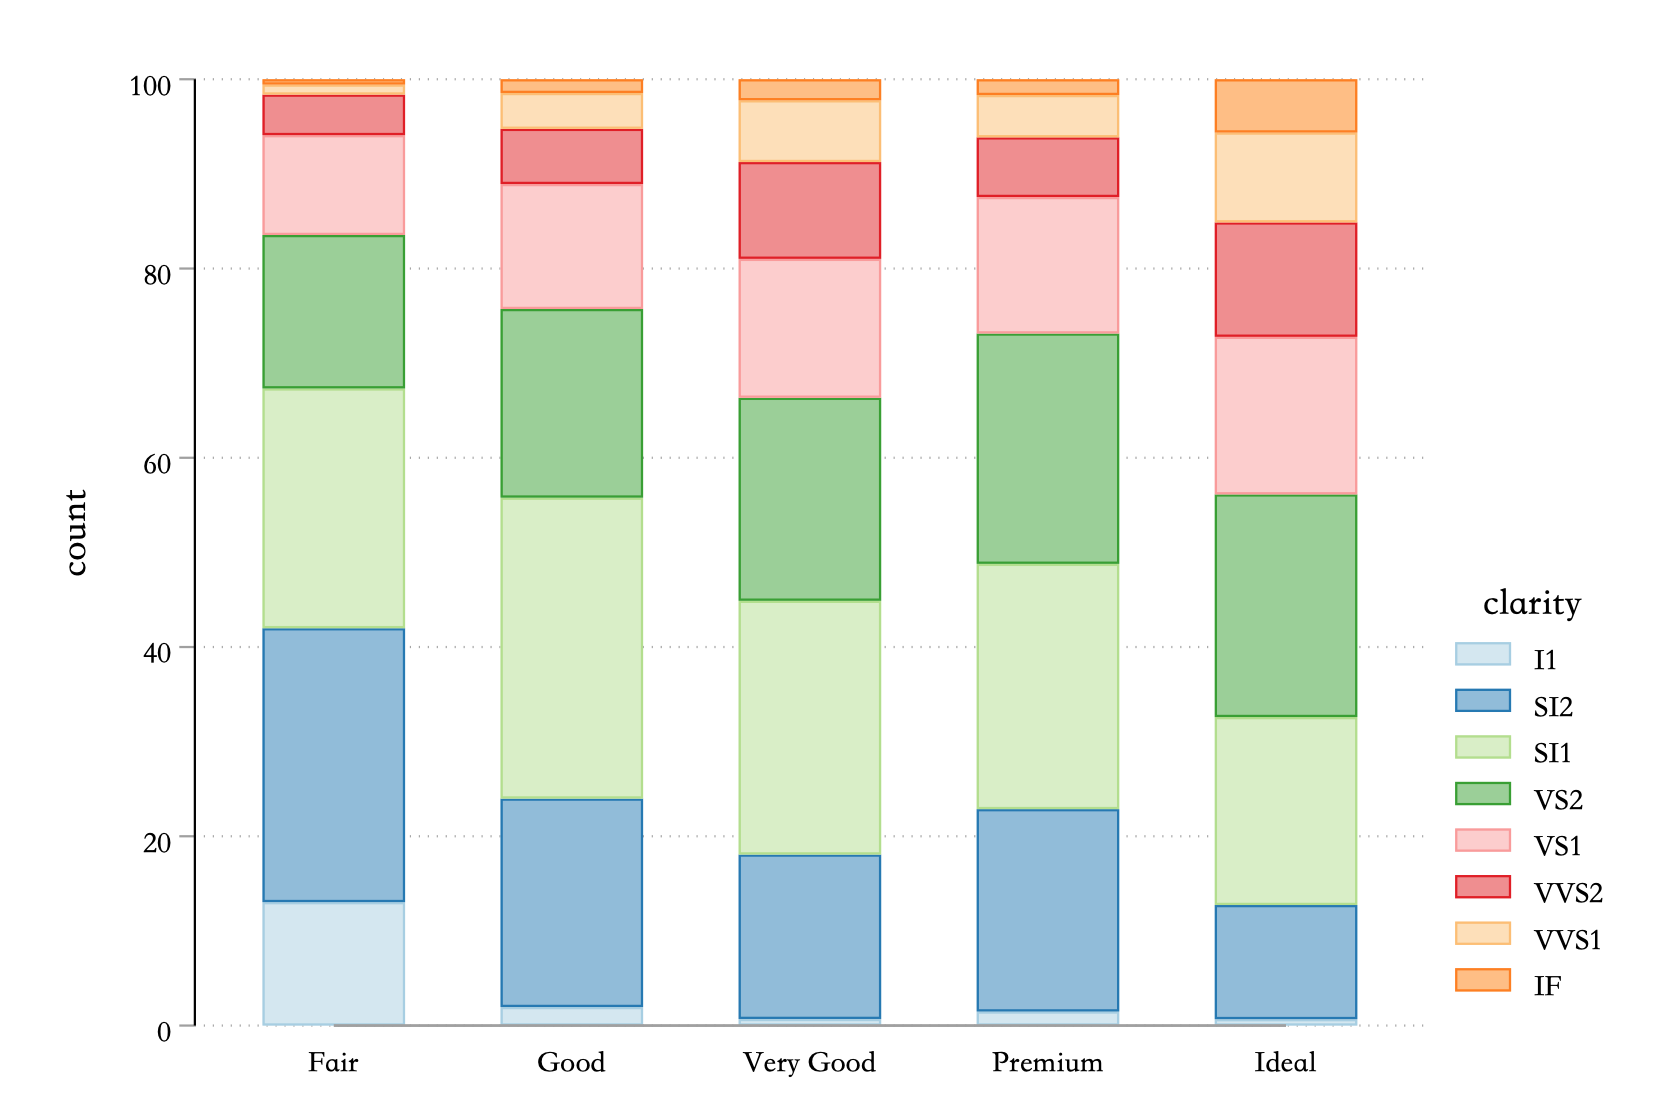
\includegraphics[width=\textwidth]{assets/percentcutclarity.png}
  \caption{钻石不同切工的克拉分布}\label{fig:percentcutclarity}
\end{figure}

最后,\textcolor{third2}{dodge} 模式为,如图 \ref{fig:dodgecutclarity}:

\begin{lstlisting}
sysuse diamonds, clear
gen id = _n
colorscheme 8, palette(Paired)
gr bar (count) id, over(clarity) over(cut) ///
    asyvars yti(count) ///
    leg(ti(clarity)) ///
    bar(1, color("`r(color1)'")) ///
    bar(2, color("`r(color2)'")) ///
    bar(3, color("`r(color3)'")) ///
    bar(4, color("`r(color4)'")) ///
    bar(5, color("`r(color5)'")) ///
    bar(6, color("`r(color6)'")) ///
    bar(7, color("`r(color7)'")) ///
    bar(8, color("`r(color8)'"))
\end{lstlisting}

\begin{figure}[htbp]
  \centering 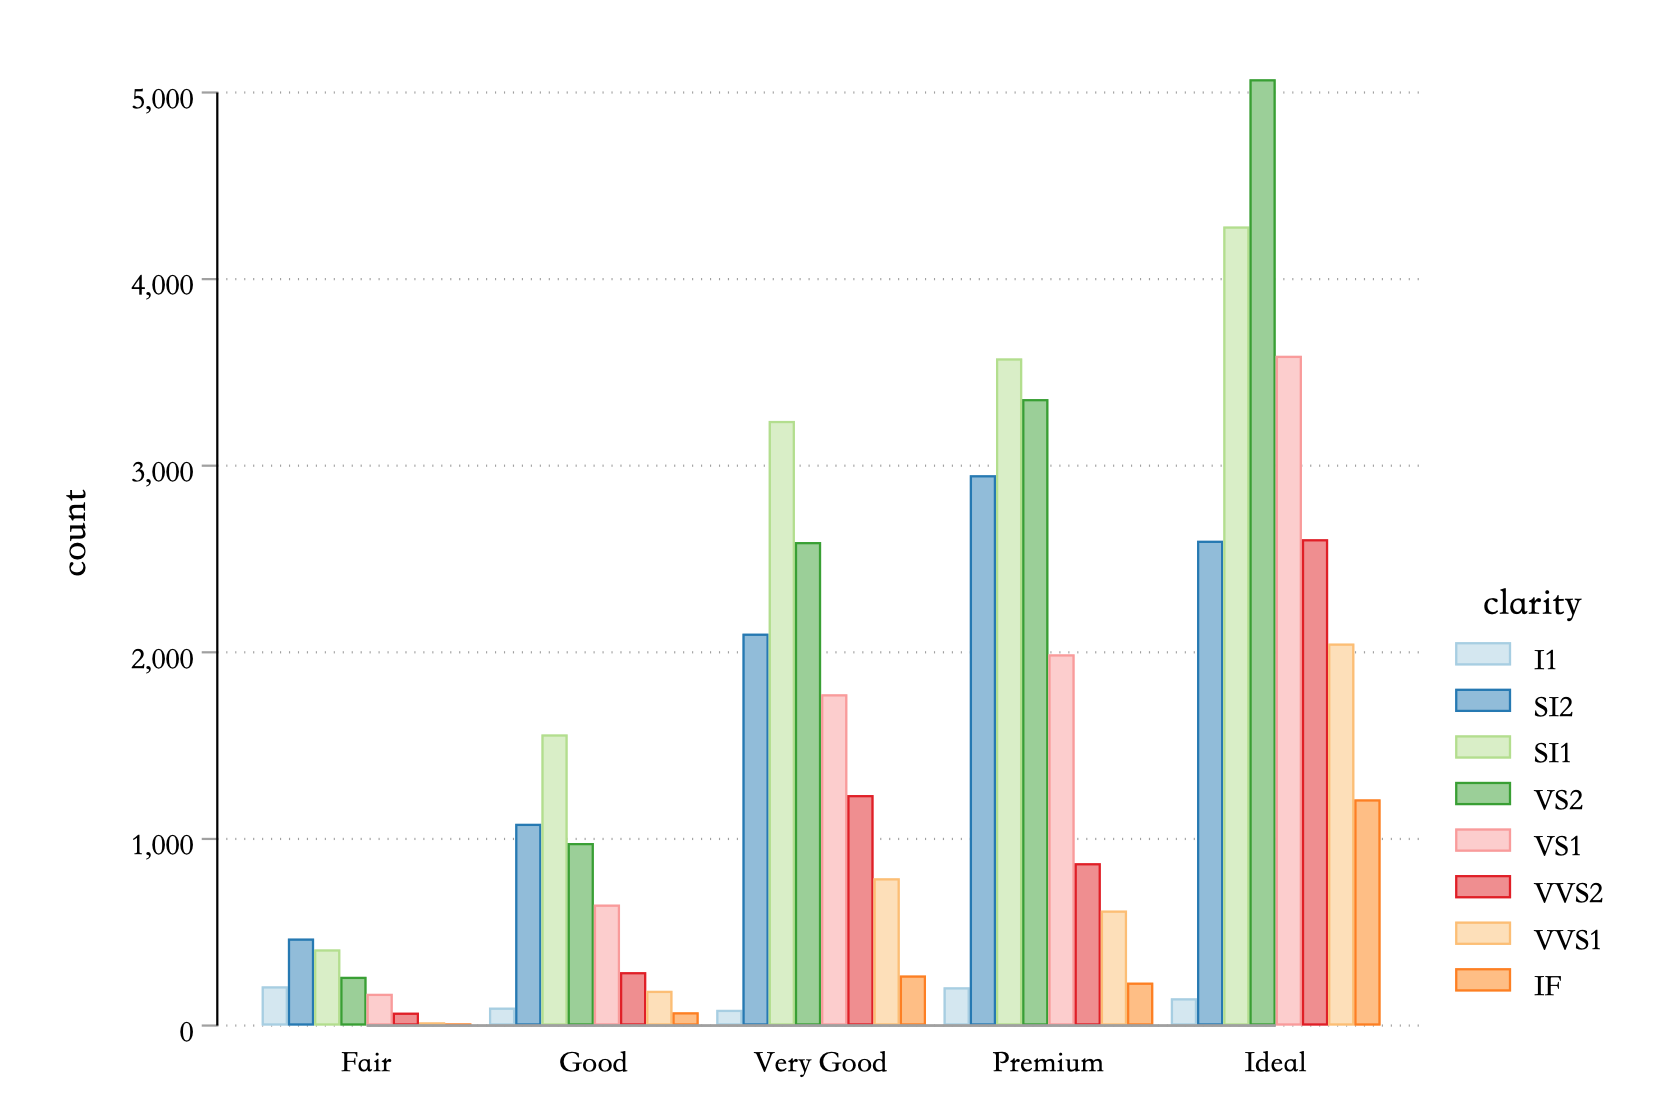
\includegraphics[width=\textwidth]{assets/dodgecutclarity.png}
  \caption{钻石不同切工的克拉分布}\label{fig:dodgecutclarity}
\end{figure}

其它类型的图其实也有位置的调整,不过不如直方图有用,例如散点图增加扰动,如图 \ref{fig:scjitter}:

\begin{lstlisting}
sysuse mpg, clear
sc hwy displ, name(p1, replace) ti(没有添加散点扰动)
sc hwy displ, name(p2, replace) jitter(3)  ti(添加了散点扰动)
gr combine p1 p2
\end{lstlisting}

\begin{figure}[htbp]
  \centering \includegraphics[width=\textwidth]{assets/scjitter.png}
  \caption{增加散点扰动的效果图}\label{fig:scjitter}
\end{figure}

很容易理解,增加散点扰动也是缓解散点重叠问题的一种办法。前面的使用透明度也是一种方法,如图 \ref{fig:scopc}。

\begin{figure}[htbp]
  \centering \includegraphics[width=\textwidth]{assets/scopc.png}
  \caption{使用透明度的效果图}\label{fig:scopc}
\end{figure}

这里再介绍两种减缓散点重叠问题的方法:

方法1: 使用 flower命令,如图 \ref{fig:flower}:

\begin{lstlisting}
* 安装:
ssc install flower
flower hwy displ
\end{lstlisting}

\begin{figure}[htbp]
  \centering \includegraphics[width=\textwidth]{assets/flower.png}
  \caption{使用太阳花的花瓣数量表示重叠程度}\label{fig:flower}
\end{figure}

实际上,Stata官方也提供了绘制太阳花的命令,如图 \ref{fig:sunflower}:

\begin{lstlisting}
sunflower hwy displ
*> Bin width          =       .36
*> Bin height         =   2.65899
*> Bin aspect ratio   =   6.39655
*> Max obs in a bin   =        12
*> Light              =         3
*> Dark               =        13
*> X-center           =       3.3
*> Y-center           =        24
*> Petal weight       =         1
*> ------------------------------------------------------------------
*>      flower      petal     No. of     No. of  estimated     actual
*>        type     weight     petals    flowers       obs.       obs.
*> ------------------------------------------------------------------
*>        none                                          46         46
*>       light          1          3          6         18         18
*>       light          1          4          7         28         28
*>       light          1          5          8         40         40
*>       light          1          6          2         12         12
*>       light          1          7          3         21         21
*>       light          1          8          2         16         16
*>       light          1          9          1          9          9
*>       light          1         10          1         10         10
*>       light          1         11          2         22         22
*>       light          1         12          1         12         12
*> ------------------------------------------------------------------
*>                                                     234        234
\end{lstlisting}

\begin{figure}[htbp]
  \centering \includegraphics[width=0.8\textwidth]{assets/sunflower.png}
  \caption{使用太阳花的花瓣数量表示重叠程度}\label{fig:sunflower}
\end{figure}

另一种方法是使用 \href{https://github.com/haghish}{E. F. Haghish} 开发的 \href{https://github.com/haghish/neat}{neat} 命令,如图 \ref{fig:neatscatter}:

\begin{lstlisting}
* 安装 neat 命令
github install haghish/neat, replace
sysuse mpg, clear
neat hwy displ
sc hwy displ
\end{lstlisting}

\begin{figure}[htbp]
  \centering
  \includegraphics[width=\textwidth]{assets/neatscatter.png}
  \caption{使用太阳花的花瓣数量表示重叠程度}\label{fig:neatscatter}
\end{figure}

需要注意的是,neat并不是绘图的命令,而是一个修改数据的命令。

关于 neat 命令的详细使用介绍可以参考其 GitHub 仓库: \href{https://github.com/haghish/neat}{haghish/neat}

\section{坐标系统}

Stata 绘图中坐标系统的调整主要是横纵坐标的交换,如图 \ref{fig:boxcombine}:

\begin{lstlisting}
sysuse mpg, clear
gr box hwy, over(class) ti("绘图命令:gr box hwy, over(class)") ///
    name(p1, replace)
gr hbox hwy, over(class)  ti("绘图命令:gr hbox hwy, over(class)") ///
    name(p2, replace)
gr combine p1 p2
\end{lstlisting}

\begin{figure}[htbp]
  \centering \includegraphics[width=\textwidth]{assets/boxcombine.png}
  \caption{竖直箱线图与水平箱线图}\label{fig:boxcombine}
\end{figure}

另一种常用的坐标系调整是纵轴和横轴尺度的比例,使用 \texttt{aspectratio()} 选项调整,例如我想设置纵轴和横轴的比例是 1:2,如图 \ref{fig:aspscatter}:

\begin{lstlisting}
sysuse mpg, clear
sc hwy displ, aspect(0.5)
\end{lstlisting}

\begin{figure}[htbp]
  \centering \includegraphics[width=\textwidth]{assets/aspscatter.png}
  \caption{aspectratio() 选项的使用}\label{fig:aspscatter}
\end{figure}

Stata 中并没有直接的坐标系转换机制(这就不像 ggplot2 中那么方便了),但是 Stata 中有绘制各种图的命令,以上展示的图基本都是基于笛卡尔坐标系的,基于极坐标系的饼图在 Stata 中可以直接使用 pie 命令绘制,如图 \ref{fig:barpluspie}:

\begin{lstlisting}
sysuse diamonds, clear
contract cut
colorscheme 5, palette(Paired)
tw ///
bar _freq cut if cut == 1, horizontal fc("`r(color1)'") lc("`r(color1)'") || ///
bar _freq cut if cut == 2, horizontal fc("`r(color2)'") lc("`r(color2)'") || ///
bar _freq cut if cut == 3, horizontal fc("`r(color3)'") lc("`r(color3)'") || ///
bar _freq cut if cut == 4, horizontal fc("`r(color4)'") lc("`r(color4)'") || ///
bar _freq cut if cut == 5, horizontal fc("`r(color5)'") lc("`r(color5)'") ///
    ylab(, val) name(p1, replace) nodraw leg(off)

sysuse diamonds, clear
colorscheme 5, palette(Paired)
gr pie, over(cut) ///
    pie(1, color("`r(color1)'")) ///
    pie(2, color("`r(color2)'")) ///
    pie(3, color("`r(color3)'")) ///
    pie(4, color("`r(color4)'")) ///
    pie(5, color("`r(color5)'")) ///
    name(p2, replace) leg(off) ///
    pl(1 name) ///
    pl(2 name) ///
    pl(3 name) ///
    pl(4 name) ///
    pl(5 name) nodraw
gr combine p1 p2
\end{lstlisting}

\begin{figure}[htbp]
  \centering \includegraphics[width=\textwidth]{assets/barpluspie.png}
  \caption{graph bar 和 graph pie 命令的使用}\label{fig:barpluspie}
\end{figure}

这里我们使用了一个新的选项 \texttt{horizontal},这个选项控制图像的水平显示。

最后我们再回到 \texttt{aspectratio()} 选项上,经常我们需要在图像中添加一条45线,例如绘制 QQ 图的时候就需要添加一条45度线,这个时候使用 \texttt{aspect(1)} 可以保证这条45度线是真的45度线,如图 \ref{fig:qnorm}:

\begin{lstlisting}
qnorm depth, aspect(1) xlab(40(10)80) ylab(40(10)80)
\end{lstlisting}

\begin{figure}[htbp]
  \centering \includegraphics[width=\textwidth]{assets/qnorm.png}
  \caption{depth 变量的 QQ 图}\label{fig:qnorm}
\end{figure}

\chapter{工作流程:基础}

相信经过前面几章的学习,你已经拥有了一定的 Stata 基础,尽管我没有讲述太多细节。当你刚开始使用 Stata 编程的时候,感到沮丧是很正常的,克服它的唯一办法就是继续努力学习。

在我们进一步讨论之前,让我们先确保你在运行 Stata 代码方面又一个坚实的基础,并且你知道一些最有用的 Stata 功能。

\section{编程的基础知识}

让我们回顾一下迄今为止省略的一些基础知识,以便尽快让你进行绘图。你可以使用 Stata 作为计算器:

\begin{lstlisting}
di 1 / 200 * 30
*> .15
di (59 + 73 + 2) / 3
*> 44.666667
di sin(c(pi) / 2)
*> 1
\end{lstlisting}

注意,在 Stata 中,有一类常量叫 c 类返回值(creturn),你可以运行 \texttt{help creturn} 查看其帮助文档,例如:

\begin{lstlisting}
sysuse mpg, clear

* 查看当前日期
di c(current_date)
*> 17 Apr 2019

* 查看当前时间
di c(current_time)
*> 09:57:47

* 查看 PLUS 文件夹的位置
di c(sysdir_plus)
*> /Users/czx/Library/Application Support/Stata/ado/plus/

* 查看当前工作目录的位置
di c(pwd)
*> /Users/czx/Documents/我的项目/stata4ds

* 查看当前数据集的观测值个数
di c(N)
*> 234

 * 查看当前数据集的变量个数
di c(k)
*> 11

* 查看当前数据集的文件名
di c(filename)
*> mpg.dta

* 查看当前绘图主题
di c(scheme)
*> plotplain

* 查看小写字母表
di c(alpha)
*> a b c d e f g h i j k l m n o p q r s t u v w x y z

* 查看大写字母表
di c(ALPHA)
*> A B C D E F G H I J K L M N O P Q R S T U V W X Y Z

* 查看简写月份表
di c(Mons)
*> Jan Feb Mar Apr May Jun Jul Aug Sep Oct Nov Dec

* 查看全称月份表
di c(Months)
*> January February March April May June July August September October November December

* 查看简写星期表
di c(Wdays)
*> Sun Mon Tue Wed Thu Fri Sat

* 查看全称星期表
di c(Weekdays)
*> Sunday Monday Tuesday Wednesday Thursday Friday Saturday
\end{lstlisting}

我们可以在自己的程序里使用这些 c 类值。例如,我想输出大小写字母表:

\begin{lstlisting}
local Aa = "Aa"
local alphanum = wordcount("`c(alpha)'")
forval i = 1/`alphanum'{
    local temp = word("`c(ALPHA)'", `i') + word("`c(alpha)'", `i')
    local Aa = "`Aa' `temp'"
}
di "`Aa'"
*> Aa Aa Bb Cc Dd Ee Ff Gg Hh Ii Jj Kk Ll Mm Nn Oo Pp Qq Rr Ss Tt Uu Vv Ww Xx Yy Zz
\end{lstlisting}

你可以使用 local 和 global 关键字创建宏变量:

\begin{lstlisting}
local x = 3 * 4
di `x'
*> 12

global x = 3 * 4
di $x
*> 12
\end{lstlisting}

Stata 中的宏变量类型还有很多,你可以运行 \lstinline{help macro} 查看帮助文档,通过前几章的学习你应该已经发现了,我最常使用的是 \lstinline{local}。

\section{Stata 的变量名}

Stata 中的变量名可以是下面这些形式的:

\begin{lstlisting}
        x
        myvar
        Myvar
        inc92
        ausländisch
        reciprocal_of_miles_per_gallon
        _odd
        _1994
\end{lstlisting}

Stata 的变量调用时可以使用通配符,这意味着下面的两段代码的作用是一样的:

\begin{lstlisting}
sysuse auto, clear
sum foreign
*>     Variable |        Obs        Mean    Std. Dev.       Min        Max
*> -------------+---------------------------------------------------------
*>      foreign |         74    .2972973    .4601885          0          1

sum for
*>     Variable |        Obs        Mean    Std. Dev.       Min        Max
*> -------------+---------------------------------------------------------
*>      foreign |         74    .2972973    .4601885          0          1

list m* in 1/5
*>    +---------------------+
*>    | make            mpg |
*>    |---------------------|
*> 1. | AMC Concord      22 |
*> 2. | AMC Pacer        17 |
*> 3. | AMC Spirit       22 |
*> 4. | Buick Century    20 |
*> 5. | Buick Electra    15 |
*>    +---------------------+
\end{lstlisting}

与变量名有关的更多内容可以运行 \lstinline{help varname} 查看帮助文档。

\section{调用函数}

Stata 中内置了很多函数,例如我们前面使用的 wordcount() 和 word()。下面我们来看一些例子:

\begin{lstlisting}
clear all
set obs 10
gen a = _n
egen b = fill(1 2 3)
egen c = seq(), from(1) to(10)
list
*>    +--------------+
*>    |  a    b    c |
*>    |--------------|
*> 1. |  1    1    1 |
*> 2. |  2    2    2 |
*> 3. |  3    3    3 |
*> 4. |  4    4    4 |
*> 5. |  5    5    5 |
*>    |--------------|
*> 6. |  6    6    6 |
*> 7. |  7    7    7 |
*> 8. |  8    8    8 |
*> 9. |  9    9    9 |
*>10. | 10   10   10 |
*>    +--------------+
\end{lstlisting}

关于 egen 函数的更多用法可以运行 \texttt{help egen} 参考其帮助文档。也可以参考我的网站文章:\href{https://www.czxa.top/posts/18884/}{Stata中的egen函数}。这篇文章几乎搜集了所有的 egen 函数。

\begin{lstlisting}
clear all
set obs 5
egen a = fill(1 3.25)
list a
*>    +------+
*>    |    a |
*>    |------|
*> 1. |    1 |
*> 2. | 3.25 |
*> 3. |  5.5 |
*> 4. | 7.75 |
*> 5. |   10 |
*>    +------+
\end{lstlisting}

\section{实践}

我曾经遇到过这样一个问题,经过对 \href{https://chfs.swufe.edu.cn/}{CHFS} 数据的处理,我得到了每个家庭的人口数、年收入,然后我想计算每个省的基尼系数。我把处理之后的数据存放在我的 cuse 数据库里面了:

\begin{lstlisting}
cuse fincome, clear web
* 或者
sysuse fincome, clear
list in 1/10
*>    +--------------------------------+
*>    |    fid   fnum   year   fincome |
*>    |--------------------------------|
*> 1. | 110003      3   2012    100000 |
*> 2. | 110006      3   2012     77180 |
*> 3. | 110009      7   2012     98200 |
*> 4. | 110011      5   2012     76000 |
*> 5. | 110013      3   2012    116000 |
*>    |--------------------------------|
*> 6. | 110015      3   2012     30000 |
*> 7. | 110020      6   2012     92000 |
*> 8. | 110021      2   2012     64800 |
*> 9. | 110022      4   2012    130000 |
*>10. | 110023      2   2012    127640 |
*>    +--------------------------------+
\end{lstlisting}

家庭变量的前两位是省份编号,我们可以使用下面的代码生成一个省份变量:

\begin{lstlisting}
tostring fid, gen(provcd)
replace provcd = substr(provcd, 1, 2)
destring provcd, replace
\end{lstlisting}

其中,\texttt{fid} 变量是家庭的编号、\texttt{fnum} 变量是家庭的人口数,\texttt{year} 是调查数据的年份,\texttt{fincome} 是该家庭的年收入。

为了计算不平等度,我们需要安装 \texttt{egen\_inequal.pkg} 命令包:

\begin{lstlisting}
net install egen_inequal.pkg, from("http://fmwww.bc.edu/RePEc/bocode/e/")
\end{lstlisting}

该命令的使用方法是:

\begin{lstlisting}
egen rmd = inequal(fincome), index(rmd) weight(fnum) by(provcd)
egen cov = inequal(fincome), index(cov) weight(fnum) by(provcd)
egen sdl = inequal(fincome), index(sdl) weight(fnum) by(provcd)
egen mehran = inequal(fincome), index(mehran) weight(fnum) by(provcd)
egen piesch = inequal(fincome), index(piesch) weight(fnum) by(provcd)
egen kakwani = inequal(fincome), index(kakwani) weight(fnum) by(provcd)
egen theil = inequal(fincome), index(theil) weight(fnum) by(provcd)
egen mld = inequal(fincome), index(mld) weight(fnum) by(provcd)
egen entropy = inequal(fincome), index(entropy) weight(fnum) by(provcd)
egen half = inequal(fincome), index(half) weight(fnum) by(provcd)
egen gini = inequal(fincome), index(gini) weight(fnum) by(provcd)
\end{lstlisting}

其中 index 选项的参数的含义见表\ref{tab:egenindex}:

\begin{table}[htbp]
  \centering
  \caption{\label{tab:egenindex} index 选项参数的含义}
  \begin{tabular}{lll}
    \toprule
    index选项的参数 & 指标含义 & 中文 \\
    \midrule
    rmd & the relative mean deviation & 相对均差 \\
    cov & the coefficient of variation & 变异系数 \\
    sdl & the standard deviation of logs & 对数标准差 \\
    gini & the Gini index & 基尼指数 \\
    mehran & the Mehran index & Mehran指数 \\
    piesch & the Piesch index & Piesch指数 \\
    kakwani & the Kakwani index & Kakwani 指数 \\
    theil & Theil entropy index & 泰尔熵指数 \\
    mld & the mean log deviation & 对数均值偏差 \\
    entropy & generalized entropy measure (GE -1) & 广义熵测度-1 \\
    half & generalized entropy measure (GE -2) & 广义熵测度-2 \\
    \bottomrule
  \end{tabular}
\end{table}

为每个省保留一个观测值:

\begin{lstlisting}
duplicates drop provcd, force
keep provcd rmd-half
\end{lstlisting}

\begin{figure}[htbp]
 \centering
 \includegraphics[width=\textwidth]{assets/gini.png}
 \caption{各省的收入不平等度度}\label{fig:gini}
\end{figure}

\chapter{数据变形}

图表是展示数据的重要工具,但是进行研究时拿到的第一手数据往往是无法直接进行绘图的,通常你需要进行适当的数据变形,例如对数据进行汇总或者生成一些新的变量。本章将介绍如何对数据进行变形。

\section{nycflights13 数据集}

这个数据集包含了2013年从纽约市出发的 336,776 个航班,这些数据集来自美国\href{http://www.transtats.bts.gov/DatabaseInfo.asp?DB_ID=120\&Link=0}{运输统计局}:

\begin{lstlisting}
use nycflights13, clear
des

*> Contains data from nycflights13.dta
*>   obs:       336,776
*>  vars:            19                          29 Apr 2019 09:57
*>  size:    34,351,152
*> ---------------------------------------------------------------
*>               storage   display    value
*> variable name   type    format     label      variable label
*> ---------------------------------------------------------------
*> year            long    %12.0g
*> month           long    %12.0g
*> day             long    %12.0g
*> dep_time        long    %12.0g
*> sched_dep_time  long    %12.0g
*> dep_delay       double  %10.0g
*> arr_time        long    %12.0g
*> sched_arr_time  long    %12.0g
*> arr_delay       double  %10.0g
*> carrier         str2    %-9s
*> flight          long    %12.0g
*> tailnum         str6    %-9s
*> origin          str3    %-9s
*> dest            str3    %-9s
*> air_time        double  %10.0g
*> distance        double  %10.0g
*> hour            double  %10.0g
*> minute          double  %10.0g
*> time_hour       double  %tc
*> ---------------------------------------------------------------
\end{lstlisting}

\section{筛选}

keep 和 drop 命令允许你对数据集进行筛选,例如我们保留1月1日的所有航班:

\begin{lstlisting}
keep if month == 1 & day == 1
* 等价于
drop if month != 1 | day != 1
\end{lstlisting}

再例如,我们保存11月和12月的航班:

\begin{lstlisting}
keep if month == 11 | month == 12
* 等价于
drop if month != 11 & month != 12
\end{lstlisting}

逻辑运算遵循 De Morgan 定律:\texttt{!(x\ \&\ y)\ 等于\ !x\ \textbar{}\ !y}

\section{缺失值}

\begin{definition}{Stata 中的缺失值}{missing}
  \begin{enumerate}
    \item Stata中有27个数值型缺失值,其中\texttt{.}是系统缺失值(system missing value)或\texttt{sysmiss},而剩下的26个\texttt{.a,\ .b,\ .c,\ ···,\ .z}被称为扩展缺失值(extended missing values),这些拓展缺失值的作用是帮助使用者更好的跟踪缺失值。
    \item Stata中字符串的缺失值只有一种,也就是""。
  \end{enumerate}
\end{definition}

\begin{property}{Stata中实数的大小顺序}
  \begin{equation}
    \texttt{非缺失值} < . < .a < .b <  ...  < .z
  \end{equation}
\end{property}

缺失值处理示例:

\begin{lstlisting}
clear all
set obs 10
gen x = .
gen y = ""
gen a = missing(x)
gen b = missing(y)
list
*>     +---------------+
*>     | x   y   a   b |
*>     |---------------|
*>  1. | .       1   1 |
*>  2. | .       1   1 |
*>  3. | .       1   1 |
*>  4. | .       1   1 |
*>  5. | .       1   1 |
*>     |---------------|
*>  6. | .       1   1 |
*>  7. | .       1   1 |
*>  8. | .       1   1 |
*>  9. | .       1   1 |
*> 10. | .       1   1 |
*>     +---------------+
\end{lstlisting}

\begin{lstlisting}
clear all
set obs 3
gen a = .
replace a = 1 in 1
replace a = 3 in 3
keep if missing(a) | a > 1
list
*>    +---+
*>    | a |
*>    |---|
*> 1. | . |
*> 2. | 3 |
*>    +---+
\end{lstlisting}

\section{排列}
\subsection{列排序}

列排序的意义不大,主要是把我们最关心的一些列排在前几列方便我们观察:

\begin{lstlisting}
use nycflights13, clear
order year month day
\end{lstlisting}

这样就能把 year month day 三个变量排在前三列了。

\subsection{行排序}

行排序可以让我们更容易看到变量的极值:

\begin{lstlisting}
* 顺序
gsort dep_time
* 逆序
gsort -dep_time
\end{lstlisting}

多变量排序:

\begin{lstlisting}
gsort dep_time -sched_dep_time
\end{lstlisting}

由于缺失值大于所有非缺失值,所以顺序排列的时候缺失值排在最后一行。

\section{选择}

选择变量同样可以使用 keep 和 drop 实现,例如只保留 year month day 变量:

\begin{lstlisting}
keep year month day
* 或者
drop dep_time - time_hour
\end{lstlisting}

\texttt{dep\_time\ -\ time\_hour} 表示 \texttt{dep\_time} 到 \texttt{time\_hour} 的所有变量。

变量选择可以使用通配符,例如保留所有开头为 a 的变量:

\begin{lstlisting}
use nycflights13, clear
keep a*
\end{lstlisting}

保留所有结尾为 y 的变量:

\begin{lstlisting}
use nycflights13, clear
keep *y
\end{lstlisting}

保留所有变量名中含 a 的变量:

\begin{lstlisting}
use nycflights13, clear
keep *a*
\end{lstlisting}

\section{变量重命名}

变量重命名使用 rename 命令,例如根据 year month day 变量生成 date 变量,再把 date 变量重命名为 \texttt{日期}:

\begin{lstlisting}
use nycflights13, clear
gen tempdate = string(year) + "-" + string(month) + "-" + string(day)
gen date = date(tempdate, "YMD")
order date
format date %tdCY-N-D
drop tempdate
ren date 日期
\end{lstlisting}

\section{生成新的变量}

\begin{lstlisting}
use nycflights13, clear
keep year - day *delay distance air_time
gen gain = dep_delay - arr_delay
gen speed = distance / air_time * 60
\end{lstlisting}

你可以继续使用刚刚生成的新列:

\begin{lstlisting}
gen hours = air_time / 60
gen gain_per_hour = gain / hours
\end{lstlisting}

一些有用的函数:

\begin{lstlisting}
use nycflights13, clear
keep dep_time
* 整除
gen hour = int(dep_time / 100)
* 取余
gen minute = mod(dep_time, 100)
\end{lstlisting}

滞后与领先:

\begin{lstlisting}
use nycflights13, clear
gen tempdate = string(year) + "-" + string(month) + "-" + string(day)
gen date = date(tempdate, "YMD")
order date
format date %tdCY-N-D
drop tempdate

duplicates drop date, force
tsset date
keep date dep_time
gen lag = l.dep_time
gen lead = f.dep_time
\end{lstlisting}

累计求和:

\begin{lstlisting}
clear all
set obs 10
gen x = _n
gen cumsum = sum(x)
gen cummean = sum(x) / x
list
*>     +----------------------+
*>     |  x   total   cummean |
*>     |----------------------|
*>  1. |  1       1         1 |
*>  2. |  2       3       1.5 |
*>  3. |  3       6         2 |
*>  4. |  4      10       2.5 |
*>  5. |  5      15         3 |
*>     |----------------------|
*>  6. |  6      21       3.5 |
*>  7. |  7      28         4 |
*>  8. |  8      36       4.5 |
*>  9. |  9      45         5 |
*> 10. | 10      55       5.5 |
*>     +----------------------+
\end{lstlisting}

排名函数:

\begin{lstlisting}
clear all
set obs 6
gen x = 2
replace x = 1 in 1
replace x = . in 4
replace x = 3 in 5
replace x = 4 in 6
egen rank1 = rank(x), field
egen rank2 = rank(x), track
egen rank3 = rank(x), unique
list

*>    +---------------------------+
*>    | x   rank1   rank2   rank3 |
*>    |---------------------------|
*> 1. | 1       5       1       1 |
*> 2. | 2       3       2       2 |
*> 3. | 2       3       2       3 |
*> 4. | .       .       .       . |
*> 5. | 3       2       4       4 |
*>    |---------------------------|
*> 6. | 4       1       5       5 |
*>    +---------------------------+
\end{lstlisting}

\section{分组汇总}

求 dep\_delay 变量的均值:

\begin{lstlisting}
use nycflights13, clear
sum dep_delay
*>     Variable |        Obs        Mean    Std. Dev.       Min        Max
*> -------------+---------------------------------------------------------
*>    dep_delay |    328,521    12.63907    40.21006        -43       1301
\end{lstlisting}

求每一天 dep\_delay 变量的均值。

方法一(tabstat):

\begin{lstlisting}
use nycflights13, clear
sum dep_delay

gen tempdate = string(year) + "-" + string(month) + "-" + string(day)
gen date = date(tempdate, "YMD")
order date
format date %tdCY-N-D
drop tempdate

tabstat dep_delay, by(date) stat(mean) nototal save

*> Summary for variables: dep_delay
*>      by categories of: date
*>      date |      mean
*> ----------+----------
*> 2013-01-01 |  11.54893
*> 2013-01-02 |  13.85882
*> 2013-01-03 |  10.98783
*> 2013-01-04 |  8.951595
*> 2013-01-05 |  5.732218
*> 2013-01-06 |  7.148014
*> 2013-01-07 |  5.417204
*> 2013-01-08 |  2.553073
*> ······
*> 2013-12-24 |  6.765957
*> 2013-12-25 |  7.552448
*> 2013-12-26 |   14.4172
*> 2013-12-27 |  10.93763
*> 2013-12-28 |   7.98155
*> 2013-12-29 |  22.30955
*> 2013-12-30 |  10.69811
*> 2013-12-31 |  6.996053
*> ---------------------
\end{lstlisting}

方法二(sumup):

\begin{lstlisting}
use nycflights13, clear
sumup dep_delay, by(year month day) statistics(mean) save(temp.dta) replace
use temp, clear
list in 1/10

*>     +-------------------------------+
*>     | year   month   day       mean |
*>     |-------------------------------|
*>  1. | 2013       1     1   11.54893 |
*>  2. | 2013       1     2   13.85882 |
*>  3. | 2013       1     3   10.98783 |
*>  4. | 2013       1     4   8.951595 |
*>  5. | 2013       1     5   5.732218 |
*>     |-------------------------------|
*>  6. | 2013       1     6   7.148015 |
*>  7. | 2013       1     7   5.417204 |
*>  8. | 2013       1     8   2.553073 |
*>  9. | 2013       1     9   2.276477 |
*> 10. | 2013       1    10   2.844995 |
*>     +-------------------------------+
\end{lstlisting}

\subsection{观察航班里程和航班延误时间的关系}

图 \ref{fig:delaydist} 展示了航班里程和航班延误时间的关系:

\begin{lstlisting}
use nycflights13, clear
bysort dest: gen count = _N
bysort dest: egen dist = mean(dist)
bysort dest: egen delay = mean(arr_delay)
keep if count > 20 & dest != "HNL"
duplicates drop dest, force

tw ///
sc delay dist [fw = count], msize(*0.3) || ///
lpoly delay dist, lc(blue) bw(300) ||, ///
leg(pos(6) order(1 "局部多项式拟合")) ///
note(散点半径表示该天的航班数)
\end{lstlisting}

这里使用 \texttt{lpoly} 命令进行局部多项式拟合,\texttt{bw()} 选项用于选择带宽,其数值越大曲线越平滑。

\begin{figure}[htbp]
  \centering
  \includegraphics[width=\textwidth]{assets/delaydist.png}
  \caption{航班里程和航班延误时间的关系}
  \label{fig:delaydist}
\end{figure}

不同于 R 语言,Stata 中不能方便的建立各种映射,这里我是使用 fw 频率权重将 count 变量展示为散点的大小。你会发现这个映射是没有图例的。

\subsection{缺失值的处理}

缺失值的处理是一件让人很为难又很灵活的事情,通常我们可以预先删除含有缺失值的变量:

\begin{lstlisting}
use nycflights13, clear
drop if missing(dep_delay) | missing(arr_delay)
bysort year month day: egen mean = mean(dep_delay)
duplicates drop year month day, force
list year month day mean in 1/5

*>    +-------------------------------+
*>    | year   month   day       mean |
*>    |-------------------------------|
*> 1. | 2013       1     1   11.43562 |
*> 2. | 2013       1     2    13.6778 |
*> 3. | 2013       1     3   10.90778 |
*> 4. | 2013       1     4   8.965859 |
*> 5. | 2013       1     5   5.732218 |
*>    +-------------------------------+
\end{lstlisting}

\subsection{观测值计数}

对数据进行分组汇总的时候,最好包括观测值的数量或非缺失观测值的数量。这样,您可以检查您的结论是否是根据非常少量的数据得出的。例如,让我们看一下不同尾号的飞机的平均延迟时间的分布,见图 \ref{fig:kdensitydelay}:

\begin{lstlisting}
use nycflights13, clear
drop if missing(dep_delay) | missing(arr_delay)
bysort tailnum: egen delay = mean(arr_delay)
duplicates drop tailnum, force
kdensity delay
\end{lstlisting}

\begin{figure}[htbp]
  \centering
  \includegraphics[width=\textwidth]{assets/kdensitydelay.png}
  \caption{不同尾号的飞机的平均延迟时间的分布}
  \label{fig:kdensitydelay}
\end{figure}

可以看到,有些型号的飞机可能延迟 \textgreater{}300 分钟!

如果我们绘制航班数量与平均延误的散点图,我们可以发现更多的东西:

\begin{lstlisting}
use nycflights13, clear
drop if missing(dep_delay) | missing(arr_delay)
bysort tailnum: egen delay = mean(arr_delay)
bysort tailnum: gen n = _N
duplicates drop tailnum, force
tw sc delay n, mc(%30)
\end{lstlisting}

\begin{figure}[htbp]
  \centering
  \includegraphics[width=\textwidth]{assets/scdelayn.png}
  \caption{航班数量与平均延误的散点图}\label{fig:scdelayn}
\end{figure}

从 \ref{fig:scdelayn} 中我们可以看到当航班很少的时候,平均延误的波动会很大,当然这其实是大数定律。

观测值很少的平均数往往是没有太多意义的,所以很多时候我们会过滤掉这些观测值很少的点:

\begin{lstlisting}
use nycflights13, clear
drop if missing(dep_delay) | missing(arr_delay)
bysort tailnum: egen delay = mean(arr_delay)
bysort tailnum: gen n = _N
duplicates drop tailnum, force
tw sc delay n if n > 25, mc(%30)
\end{lstlisting}

\begin{figure}[htbp]
  \centering
  \includegraphics[width=\textwidth]{assets/scdelayn2.png}
  \caption{航班数量与平均延误的散点图(过滤掉观测值很少的散点)}
  \label{fig:scdelayn2}
\end{figure}

这种模式还有另一种常见的变化。让我们来看看棒球击球手的平均表现如何与他们击球的次数有关:

\begin{lstlisting}
use batting, clear
bysort playerID: egen temp1 = sum(H)
bysort playerID: egen temp2 = sum(AB)
gen ba = temp1 / temp2
bysort playerID: egen ab = sum(AB)
drop temp*
keep if ab > 100
duplicates drop playerID, force
tw ///
sc ba ab, mc(%30) || ///
lpoly ba ab, lc(blue) ||, ///
leg(pos(6) rows(1))
\end{lstlisting}

\begin{figure}[htbp]
  \centering
  \includegraphics[width=\textwidth]{assets/scbaab.png}
  \caption{棒球击球手的平均表现与他们击球的次数的关系}
  \label{fig:scbaab}
\end{figure}

可以看到,击球次数越多的击球手表现越稳定,表现也越好。

\subsection{有用的汇总函数}

这部分内容可以参考 Stata 的相关帮助文档:

\begin{lstlisting}
help egen
search egenmore
search egenmisc
\end{lstlisting}

或者参考我的网站博客:\href{https://www.czxa.top/posts/18884/}{Stata中的egen函数}。

\subsection{按多变量分组}

前文中我大量使用了 by/bysort 进行分组聚合,关于 by/bysort 的更多用法可以参考帮助文档:\texttt{help by}。

\chapter{探索性数据分析}

本章将会向你展示如何使用数据变形和绘图探索数据。统计学家称之为探索性数据分析或 \texttt{EDA}。EDA 实际上是个循环的工作,在 EDA 中你经常需要重复下面的三个环节:

\begin{enumerate}
\item 提出有关数据的问题;
\item 通过数据处理和可视化搜寻答案;
\item 使用你搜寻到的答案提出新的问题。
\end{enumerate}

EDA 并没有一个正规的流程。最重要的是,EDA 是一种好的工作习惯,它可以帮助你了解数据,发现一些简单想法的答案。在 EDA 的初始阶段,你可以随意探索一些你觉得有意思的问题,其中有一些想法你会得到正确的答案,而有些则会失败。

EDA 是任何数据分析的重要组成部分。要进行数据清理,你需要部署 EDA 的所有工具:可视化、转形和建模。

\section{问题}

在 EDA 期间的目标是了解数据。最简单的方法是使用问题作为指导探索的工具。当你提出问题的时候,问题会将你的注意力集中在数据机的特定部分,并帮助你的确定要生成的图形、模型。

EDA 从根本上来说是一个创造性的过程。在分析开始的时候很难提出问题,因为你不知道数据集中包含哪些信息。另一方面,你提出的每个新问题都会让你了解数据中包含的新信息,并且增加你发掘信息的机会。你可以快速深入查看数据中最有趣的部分,并开发一组发人深省的问题------如果你根据所发现的内容跟进每个问题并提出新问题。

有两种类型的问题对于数据探索是非常有用的:
\begin{enumerate}
  \item 我的变量中出现了什么类型的变化?
  \item 我的变量之间发生了什么类型的协变?
\end{enumerate}

本章的其余部分将讨论这两个问题。我将解释变异和协变是什么,我将向你展示几种回答每个问题的方法。

\section{变化}
\subsection{可视化分布}

如何可视化变量的分布取决于变量是分类变量还是连续变量。如果变量只能采用一小组值中的一个,则该变量是分类的。在 R 中,分类变量通常保存为因子或字符变量。要检查分类变量的分布,可以使用条形图,绘图结果见图 \ref{fig:histogramcut}。

\begin{lstlisting}
use diamonds, clear
histogram cut, freq barwidth(0.8)
\end{lstlisting}

\begin{figure}[htbp]
  \centering
  \includegraphics[width=\textwidth]{assets/histogramcut.png}
  \caption{cut 变量的分布}
  \label{fig:histogramcut}
\end{figure}

由于这里我设定了 \texttt{freq} 选项,所以纵轴显示的是频数。另外你也可以手动计算 cut 变量每个因子的观测值的数目然后绘图:

\begin{lstlisting}
use diamonds, clear
contract cut
tw bar _freq cut
\end{lstlisting}

\begin{figure}[htbp]
  \centering
  \includegraphics[width=\textwidth]{assets/histogramcut2.png}
  \caption{cut 变量的分布}
  \label{fig:histogramcut2}
\end{figure}

如果变量可以在连续集上进行取值,那么该变量就是连续的。数字和日期变量就是连续变量的两个例子。要检查连续变量的分布,请使用直方图:

\begin{lstlisting}
use diamonds, clear
hist carat, freq
\end{lstlisting}

\begin{figure}[htbp]
  \centering
  \includegraphics[width=\textwidth]{assets/histcarat.png}
  \caption{carat 变量的分布}\label{fig:histcarat}
\end{figure}

你可以使用 \texttt{width(0.5)} 指定每组组宽为 0.5 :

\begin{lstlisting}
hist carat, freq width(0.5)
\end{lstlisting}

\begin{figure}[htbp]
  \centering
  \includegraphics[width=\textwidth]{assets/histcarat2.png}
  \caption{carat 变量的分布}
  \label{fig:histcarat2}
\end{figure}

直方图将 x 轴分成等间距的箱,然后使用条的高度显示每个箱子中的观测数。在上图中,最高的条形显示近 3000 个观测值的 carat 变量值介于 0.25 和 0.75 之间,这是条形图的左右边界。

\texttt{width()} 选项可以用来设置组宽,该选项是以 x 变量为单位进行测量的。在使用直方图的时候,你应该始终探索各种带宽,因为不同的宽度可以揭示不同的模式,例如图\ref{fig:histsmallercarat}是我们放大 carat \textless{} 3 的钻石并选择较小的宽度绘制的直方图:

\begin{lstlisting}
use diamonds, clear
keep if carat < 3
hist carat, width(0.1)
\end{lstlisting}

\begin{figure}[htbp]
  \centering
  \includegraphics[width=\textwidth]{assets/histsmallercarat.png}
  \caption{carat < 3 子集中 carat 变量的分布}
  \label{fig:histsmallercarat}
\end{figure}

在同一幅图中叠加多个直方图是不好的,建议使用 kdensity 命令:

\begin{lstlisting}
use diamonds, clear
keep carat cut
colorscheme 5, palette(Paired)
tw ///
kdensity carat if cut == 1, lc("`r(color1)'") lp(solid) || ///
kdensity carat if cut == 2, lc("`r(color2)'") lp(solid) || ///
kdensity carat if cut == 3, lc("`r(color3)'") lp(solid) || ///
kdensity carat if cut == 4, lc("`r(color4)'") lp(solid) || ///
kdensity carat if cut == 5, lc("`r(color5)'") lp(solid) ||, ///
leg(order(1 "Fair" 2 "Good" 3 "Very Good" 4 "Premium" 5 "Ideal")) ///
xti("carat") yti("density") ylab(, format(%6.2f))
\end{lstlisting}

\begin{figure}[htbp]
  \centering
  \includegraphics[width=\textwidth]{assets/kdensitycarat.png}
  \caption{carat 变量的核密度分布}
  \label{fig:kdensitycarat}
\end{figure}


\nocite{ggplot2, R-base, R-bookdown, R-knitr, R-rmarkdown, xie2015, r4ds, stata, github,neat,haven,stata4ds, stcolor,cuse,finance,dict,stata2docx,stata-colorscheme,plotplain,tidy,flower}
\bibliography{reference}
\end{document}
